\documentclass[a4paper, 12pt, oneside]{Thesis}  % Use the "Thesis" style, based on the ECS Thesis style by Steve Gunn
\graphicspath{{figure/}}  % Location of the graphics files (set up for graphics to be in PDF format)
\usepackage[square, numbers, comma, sort&compress]{natbib}  % Use the "Natbib" style for the references in the Bibliography
\usepackage{verbatim}  % Needed for the "comment" environment to make LaTeX comments
\usepackage{vector}  % Allows "\bvec{}" and "\buvec{}" for "blackboard" style bold vectors in maths

\usepackage{url}
\usepackage{multirow}
\usepackage{algorithm}
\usepackage{lscape}
\usepackage{rotating}
\usepackage{caption}
\usepackage{algpseudocode}
\usepackage{mathtools}

\usepackage{appendix}
\usepackage{graphicx}
\usepackage{caption}
\usepackage{subcaption}
\usepackage{sectsty}
\usepackage[at]{easylist}
\usepackage[dvipsnames]{xcolor}
\usepackage{gensymb}
\chapterfont{\centering\MakeUppercase}

\newcommand\NoDo{\renewcommand\algorithmicdo{}}
\DeclarePairedDelimiter\ceil{\lceil}{\rceil}
\DeclarePairedDelimiter\floor{\lfloor}{\rfloor}
\hypersetup{urlcolor=black, colorlinks=true}  % Colours hyperlinks in blue, but this can be distracting if there are many links.

%% ----------------------------------------------------------------


\begin{document}
\frontmatter	  % Begin Roman style (i, ii, iii, iv...) page numbering
\begin{titlepage}
   \begin{center}
       \vspace{1cm}
       \Huge
       \textbf{An Embedded Approach to Fall Detection and Human Activity Recognition using Wi-Fi Channel State Information}
        
      \normalsize    
       \vspace{0.5cm}
        (This project report has been submitted in partial fulfillment of the requirements for the degree of Bachelor of Science in Electrical and Electronic Engineering)
            
       \vspace{1.5cm}
       
\includegraphics[width=3.5cm, height=4cm]{university.png}
       
       \Large
       \vspace{1cm}
       \textbf{Submitted By}    
       
       
       \large
       \textbf{Exam Roll: 63969}\hfill \textbf{Exam Roll: 63949} 
       
       \textbf{Reg No: 2017614892}\hfill \textbf{Reg No: 2017114842}
       
       \textbf{Session: 2017-18}\hfill \textbf{Session: 2017-18}
       
       \vspace{1cm}
       
       \textbf{Dept. of Electrical and Electronic Engineering}
       
       \textbf{University of Dhaka}

        \textbf{June 27, 2022}
       
       
   \end{center}
\end{titlepage}

%% ----------------------------------------------------------------

\setstretch{1.2}  % It is better to have smaller font and larger line spacing than the other way round

% Define the page headers using the FancyHdr package and set up for one-sided printing
\fancyhead{}  % Clears all page headers and footers
\rhead{\thepage}  % Sets the right side header to show the page number
\lhead{}  % Clears the left side page header

\pagestyle{fancy}  % Finally, use the "fancy" page style to implement the FancyHdr headers


\addtotoc{Abstract}  % Add the "Abstract" page entry to the Contents
\addtocontents{toc}{\vspace{1em}}  % Add a gap in the Contents, for aesthetics

\title{}
\abstract{
Fall detection is an essential part of any elderly or patient assistance system. Human activity recognition techniques are widely used to implement fall detection systems. Most solutions employ wearable devices or cameras to collect data, both of which possess various critical drawbacks. We propose a device-free fall detection system using WiFi channel state information(CSI) which lacks the drawbacks of mentioned solutions yet provides competitive performance. We used two embedded devices(ESP32) to collect CSI (Channel State Information) as an embedded approach provides more flexibility in case of deployment. We recorded data while 13 volunteers performed various tasks. After rigorous preprocessing involving re-sampling, phase calibration, amplitude denoising, filtering, feature extraction, feature selection, and classification, we were able to achieve an F1 score of 98.5\% in 10-fold cross-validation for fall detection and 96.9\% for human activity recognition.
}

\clearpage  % Abstract ended, start a new page
%% ----------------------------------------------------------------

\setstretch{1.3}  % Reset the line-spacing to 1.3 for body text (if it has changed)



\setstretch{1.5}  % Set the line spacing to 1.5, this makes the following tables easier to read
\clearpage  % Start a new page


\clearpage
\pagestyle{fancy}  %The page style headers have been "empty" all this time, now use the "fancy" headers as defined before to bring them back


%% ----------------------------------------------------------------
\lhead{\emph{Contents}}  % Set the left side page header to "Contents"
\tableofcontents  % Write out the Table of Contents

%% ----------------------------------------------------------------
\lhead{\emph{List of Figures}}  % Set the left side page header to "List if Figures"
\listoffigures  % Write out the List of Figures

%% ----------------------------------------------------------------
\lhead{\emph{List of Tables}}  % Set the left side page header to "List of Tables"
\listoftables  % Write out the List of Tables



\setstretch{1.4}  % Return the line spacing back to 1.3

\pagestyle{empty}  % Page style needs to be empty for this page
%\dedicatory{For/Dedicated to/To my\ldots}

\addtocontents{toc}{\vspace{1em}}  % Add a gap in the Contents, for aesthetics


%% ----------------------------------------------------------------
\mainmatter	  % Begin normal, numeric (1,2,3...) page numbering
\pagestyle{fancy}  % Return the page headers back to the "fancy" style


\chapter{INTRODUCTION}
 \label{Chapter 1}
 \lhead{ Chapter 1. \emph{Introduction}}
\label{intro}

Healthcare has always been a fundamental concern for human society, and it is especially needed for the sick and the elderly. The percentage of persons aged over 65 was 9\% in 2020, with the rate being as high as 28\% in a single country \cite{WB:2020}. For an elderly person or a sick patient, falling can be devastating, and immediate attention is required in such a scenario. The development of fall detection systems is essential for this reason. Although many fall detection systems exist today, most of them are based on wearable devices or computer vision, which have some critical drawbacks, caused by the fundamental nature of the systems. This project is aimed to provide a non-contact fall detection system that is free of those drawbacks and is yet as effective as the existing solutions. Furthermore, we use embedded devices as this makes the system highly modifiable, deployable in many different environments, and comparatively affordable. 


\section{Motivation}

Sensor-based activity detection requires the user to wear a device containing the sensors in many cases\cite{7841080}. Some methods use computer vision for the task, which requires a camera to collect video or image data\cite{visionFall}. Although these methods can detect a fall incident quite accurately, some issues caused by these methods can make implementing them in real-world scenario a challenge. The issues faced while implementing solutions based on these methods are: 


\begin{itemize}
\item A wearable device can be perceived as uncomfortable, causing unwillingness to use them.
\item Remembering to wear a device every day can be an issue for elderly people.
\item A wearable device is more prone to wear and tear than a stationary device.
\item A camera-based solution can be both computationally and monetarily expensive.
\item A camera-based solution cannot provide reliability in adverse lighting conditions.
\end{itemize}

Comfort is of utmost importance for the elderly and the sick. A user might be understandably unwilling to wear a device if it is uncomfortable for them. Even if a system is perfectly capable of performing its assigned task, implementing it is challenging, if not impossible when the users are not willing to cooperate. Also to have a widespread application of a system, cost and durability have to be considered, especially in developing countries. So, in this project, we aim to create a non-contact fall detection system using wifi channel state information that is more comfortable, more reliable, and less costly.


\section{Objectives}

 We aim to build a non-contact fall detection system for monitoring the elderly and the sick. The objectives we aim to achieve are as follows:

\begin{itemize}
\item Implementing a system that can detect if a person in its area of operation has fallen down
\item Ensuring comfort by eliminating the need for wearing any device
\item Creating a dataset of channel state information recorded during different activities including fall
\item Recognition of different human activities using Wi-Fi channel state information to facilitate future improvement opportunities
\item Implementing a system to detect if the area of operation is empty
\item Ensuring that the system is easy to deploy and affordable by using embedded devices
\end{itemize}


\chapter{RELATED WORKS}
\label{Chapter 2}
\lhead{Chapter 2. \emph{Related Works}}

\section{Device Free Human Activity Recognition using WiFi Channel State Information}
In this study \cite{9060143}, the authors implemented an activity detection system using wifi channel state information. They were able to detect human activities like Walk, Stand, Sit, Run, etc. in a Line of Sight scenario (LOS) and a Non-Line of Sight (N-LOS) scenario within an indoor environment. They used two algorithms for classification, Support Vector Machine (SVM) and Long Short-Term Memory (LSTM) recurrent neural network. To collect the data, they used Intel WiFi Link 5300 Network Interface Card (NIC). This card supports the 802.11n standard and hence makes it possible to record channel state information. There are 64 subcarriers in 20 MHz channel and 128 subcarriers in 40 MHz channel. Two Lenovo laptops were used which were equipped with Intel WiFi Link 5300 Network Interface Card (NIC). The operating system on said laptops was 64 Bit Ubuntu version 14.04 LTS. The kernel version was 4.2.0-42. They modified the hardware using instructions provided by  Halperin et al. \cite{10.1145/1925861.1925870} who proposed the ‘Linux 802.11n CSI Tool”. For classification with SVM, they performed preprocessing and feature extraction using Discrete Wavelet Transform (DWT), Principal Component Analysis (PCA), etc, and then used the classifier. For classification with LSTM, only CSI-extraction and denoising were done. They achieved results where precision, recall, and F1 score were 95, 98, and 96 respectively for their best model.
\begin{figure}[H]
\centering
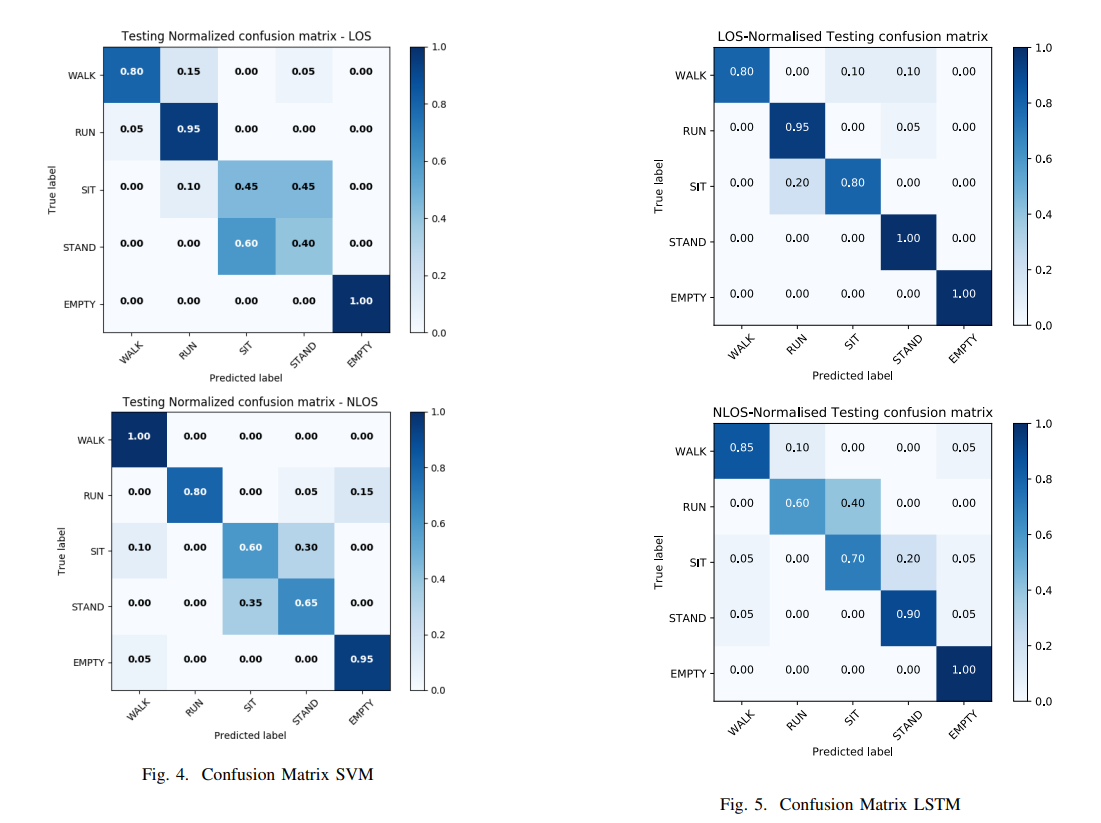
\includegraphics[width=1\textwidth]{./figure/chap 2/figure-1.png}
\caption{Confusion matrices in the paper}
\label{2.1}
\end{figure}

\textbf{There are some limitations in this method:}

\begin{itemize}
\item The hardware used for the experiment was two laptops, making this solution impractical for use in a real-world scenario. 
\item The system shows lower accuracy in detecting activities involving slow movement, like sitting or walking.
\item The system does not generalize for different environments.
\end{itemize}



\section{Wi-Motion: A Robust Human Activity Recognition Using WiFi Signals}
This study \cite{8873550}proposes a wifi-based human activity recognition system, Wi-Motion. The authors were able to classify five different pre-defined activities with impressive accuracy. The system showed a 96\% accuracy in line of sight arrangement and 92\% accuracy in non-line of sight arrangement. Furthermore, the authors evaluate the effect of the age of the experimental subjects and relatively complex environments. Wi-Motion jointly leverages the amplitude and phase information extracted from the CSI sequence. The authors first construct the classifiers using amplitude and phase, respectively. The output of classifiers is then combined by a posterior probability-based combination strategy. The authors used a commercial Tp-Link wireless router as the transmitter operating in the IEEE 802.11n AP mode at 2.4GHz. An Acer Aspire EC laptop running Ubuntu 14.04 was used as a receiver, which is equipped with an off-the-shelf Intel 5300 card (three antennas) and a modified firmware. During the process of receiving WiFi signals, the receiver pings the router 33 pkts/s and records the CSI of each packet. For each activity in different environments, every user provides 30 instances to evaluate the performance of their system. Two complex office environments were selected for data collection and 6 participants provided the data. They extracted amplitude features using DWT (Discrete Wavelet Transform). The phase feature extraction is done using WMA method and PCA. The authors use a support vector machine (SVM) algorithm for the classification of the five activities:
\begin{enumerate}
    \item Bend
    \item Halve squat
    \item Step
    \item Stretch leg
    \item Jump
\end{enumerate}

The authors also showed that the system provided accuracy higher than 80\% even when there were multiple users present. Moreover, they showed with their analysis that  during the process of data collection,
the physiological function of the person decays as the age increases, which makes the movement slower and difficult to control in a stable situation.

\begin{figure}[H]
\centering
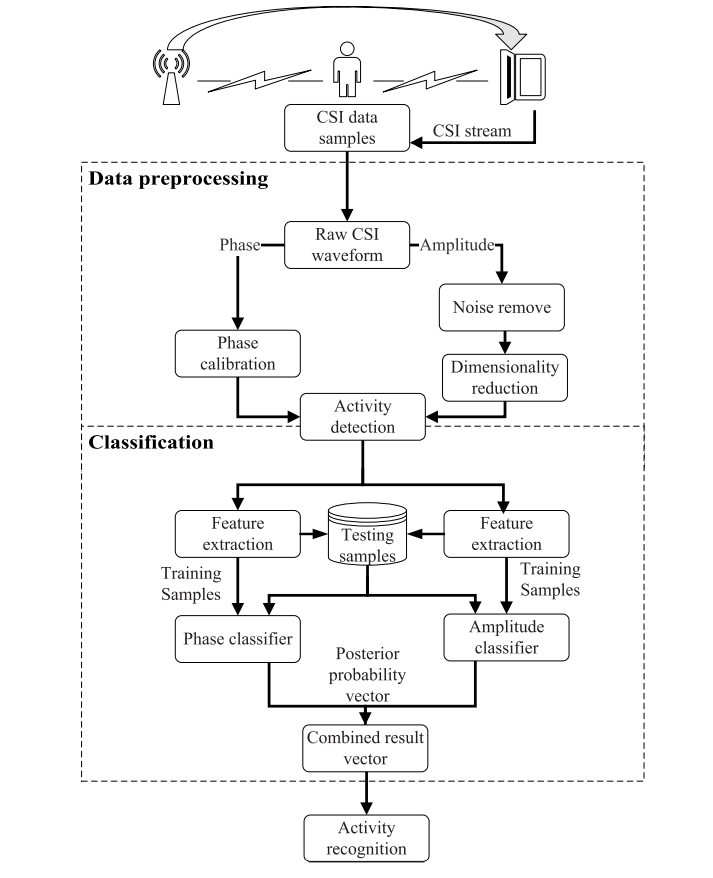
\includegraphics[width=1.0\textwidth]{./figure/chap 2/2.png}
\caption{System structure for Wi-Motion}
\label{2.2}
\end{figure}


\begin{figure}[H]
\centering
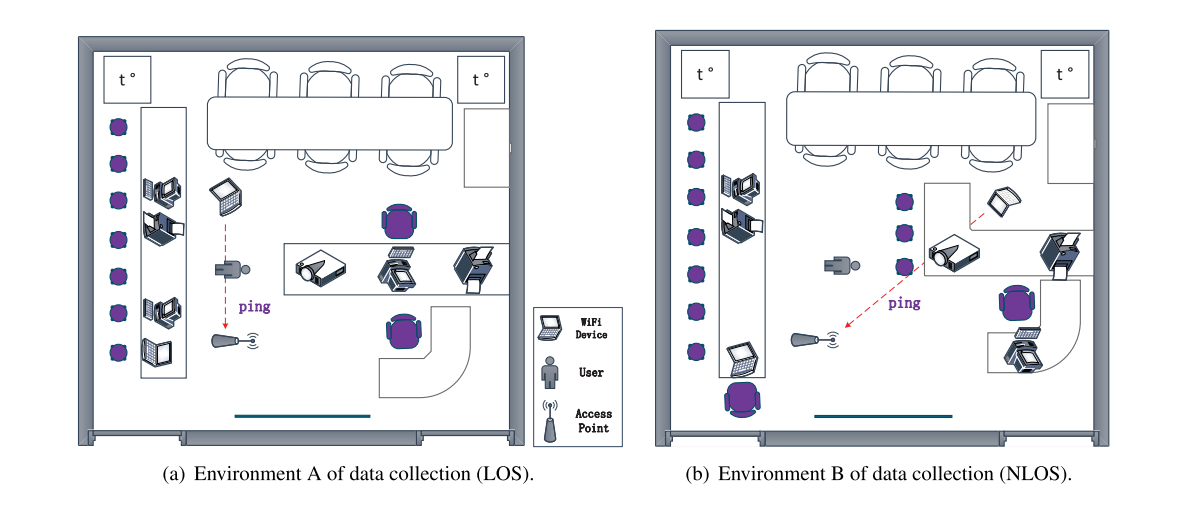
\includegraphics[width=1.0\textwidth]{./figure/chap 2/3.png}
\caption{Environment set of data collection.}
\label{2.3}
\end{figure}
 
 \textbf{Limitations:}

\begin{itemize}
\item The hardware used for the experiment were two laptops, making this solution impractical for use in a real-world scenerio. 
\end{itemize}

\section{MultiSense: Enabling Multi-person Respiration Sensing with Commodity WiFi}
The study \cite{10.1145/3411816} proposes Multisense, a WiFi-based system that can continuously
sense the detailed respiration patterns of multiple persons. It can provide a robust performance even if they have very similar respiration rates and are physically closely located. The main contributions of the paper are as follows:
\begin{itemize}
    \item The authors offered a novel method for canceling out the time-varying phase offset of WiFi CSI without distorting the linear mixture. 
    \item They showed that respiration sensing can be treated as a BSS problem that the ICA approach can efficiently address.
    \item They put MultiSense on common WiFi devices and ran comprehensive tests to see how well it works.
\end{itemize}

The authors collected CSI data using the CSI tool \cite{7010501}, which reports the complex-valued CSI samples for each received packet and can be used to collect CSI data from the receiver. For reporting CSI, the Intel 5300 WiFi card in the receiver is set to run at 5.24 GHz with a sample rate of 200 Hz and provides CSI information on 30 sub-carriers. The transmitter and receiver are both equipped with three antennas unless otherwise noted.

\begin{figure}[H]
\centering
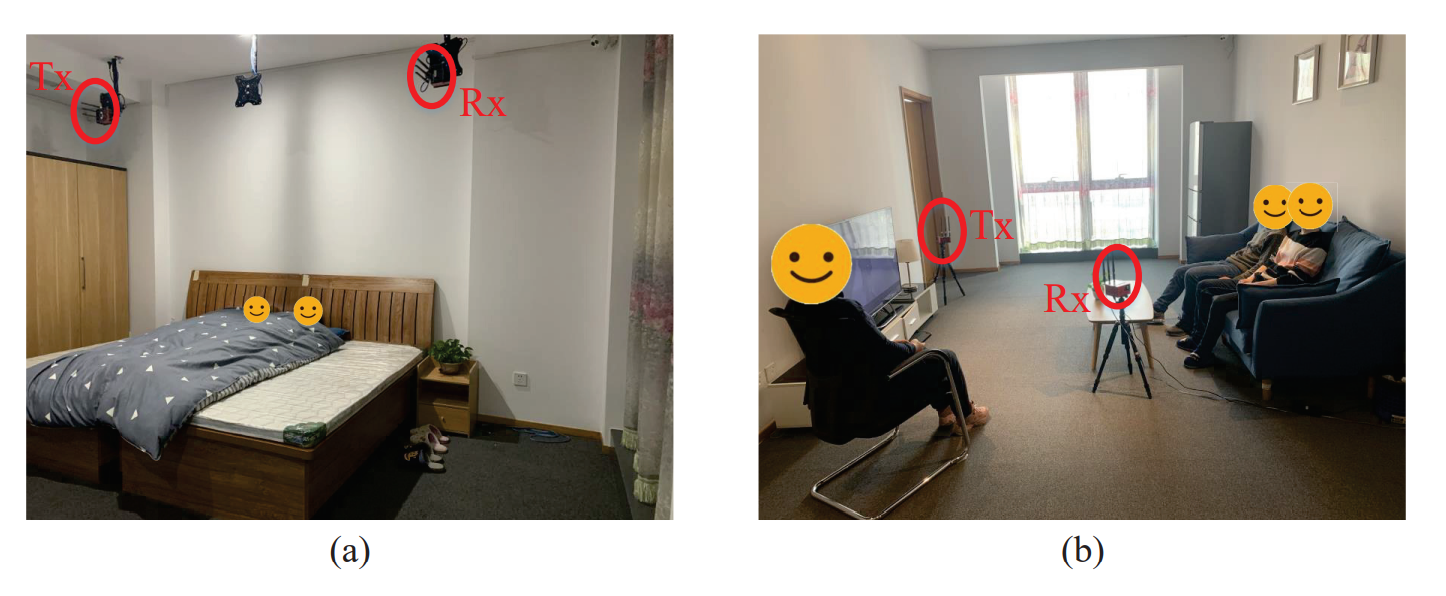
\includegraphics[width=1.0\textwidth]{./figure/chap 2/4.png}
\caption{The experimental setup in two scenarios: (a) all subjects sleep on a bed in the bedroom;
(b) each subject sits on a couch or chair in the living room.}
\label{2.4}
\end{figure}

The authors used ICA (Independent Component Analysis) to separate the breathing patterns of different persons. The added time-varying phase offset (t) and background static signals affect CSI from commodity WiFi. As a result, using raw CSI retrieved from commodity WiFi equipment, the authors were unable to use ICA to distinguish multi-person respiration signals. To overcome this, they proposed a novel method where they canceled the time-variant phase offset and removed the background static signal. Even in the presence of four people and only a pair of Wi-Fi transceivers, MultiSense is quite accurate, with a mean absolute respiration rate inaccuracy of 0.73 bpm.

\begin{figure}[H]
\centering
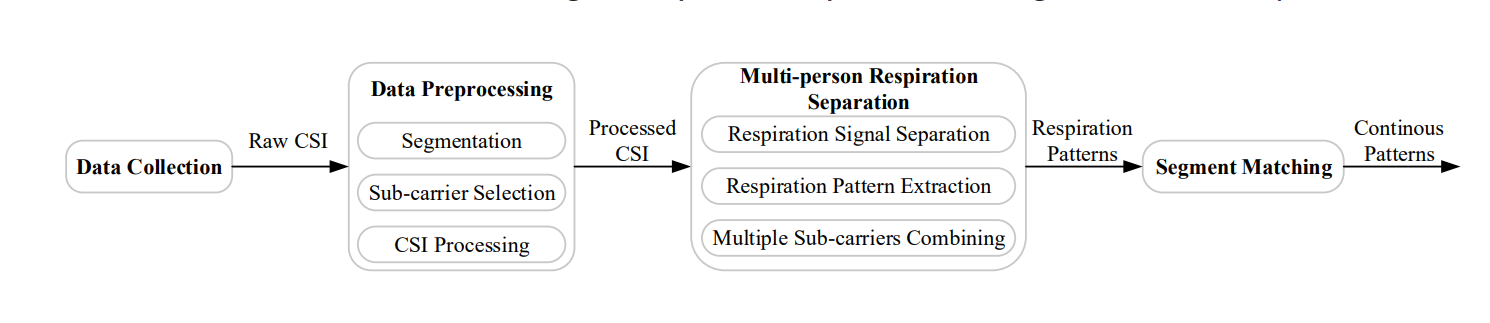
\includegraphics[width=1.0\textwidth]{./figure/chap 2/5.png}
\caption{The MultiSense system overview.}
\label{2.5}
\end{figure}

 \textbf{Limitations:}

\begin{itemize}
\item When performing blind source separation using ICA method, the number of persons is required as the input as an inherent characteristic of ICA is that it cannot identify the actual number of source signals in general. 
\item The system is not able to assign the breathing patterns to users in the case of multiple persons.
\end{itemize}

\section{A Wireless-Vision Dataset for Privacy Preserving Human Activity Recognition}
This study \cite{9264288} proposes a new WiFi-based and video-based neural network (WiNN) to improve the robustness of activity recognition where the synchronized video serves as the supplement for the wireless data. In three different visual circumstances, including scenes without occlusion, partial occlusion, and full occlusion, a wireless-vision benchmark (WiVi) is gathered for 9 class actions recognition. The accuracy of the data set is verified using both machine learning methods - support vector machine (SVM) and deep learning methods. The authors show that the WiVi data set meets the primary demand and that all three branches of the proposed pipeline maintain accuracy of more than 80\% for multiple action segmentation from 1s to 3s. 

\begin{figure}[H]
\centering
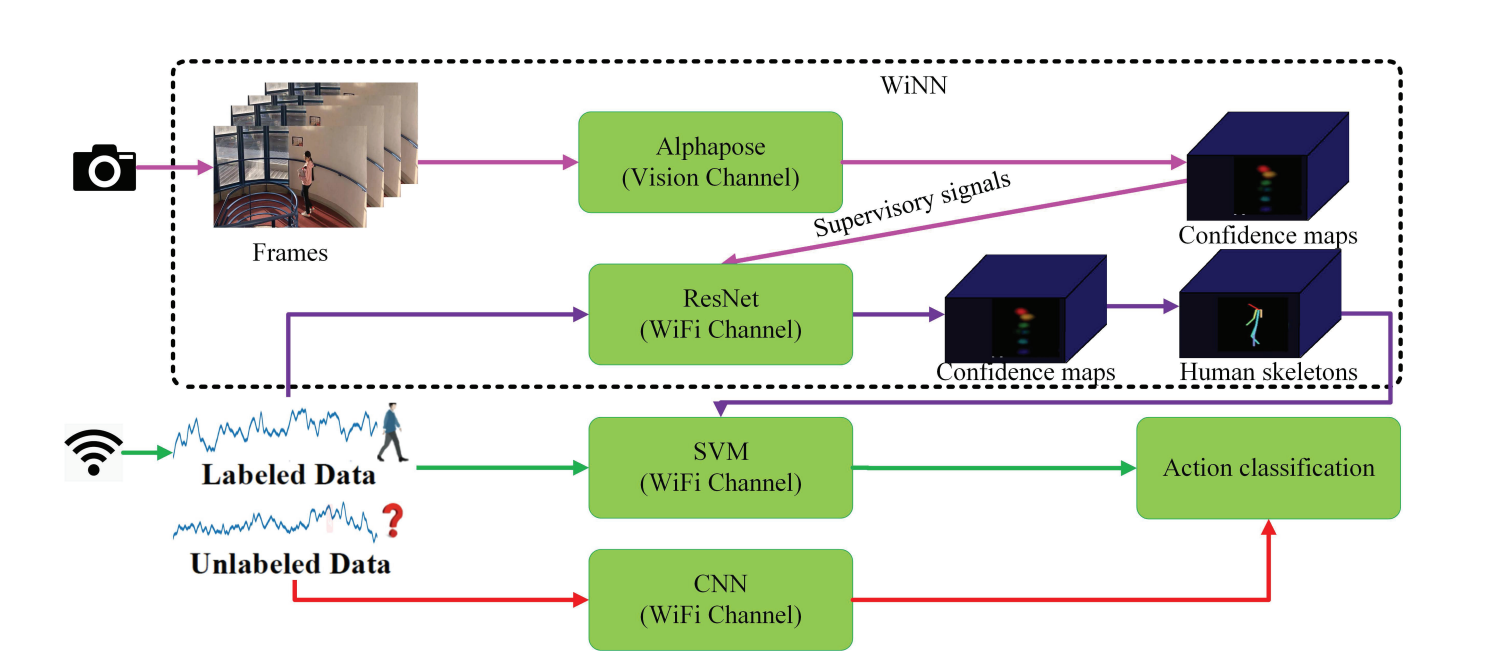
\includegraphics[width=1\textwidth]{./figure/chap 2/6.png}
\caption{The flowchart of the network for WiVi dataset.}
\label{Fig 2.6}
\end{figure}

The contribution of the paper can be summarized by the following points:

\begin{itemize}
    \item To test the effectiveness of existing activity identification systems, the authors first created WiVi, a wireless-vision activity data set. To verify the WiVi dataset's effectiveness, they used SVM, Convolutional Neural Networks (CNN), and WiNN.
    \item The authors proposed the WiNN, a WiFi-based and video-based neural network for activity recognition in partial and full occlusion scenarios, which improves the robustness of activity recognition using synchronous video as a supplement and complement to WiFi CSI signals.
    \item To verify the quality of the WiVi data set, the authors compared the machine learning method SVM with the deep learning methods CNN and WiNN. WiNN, in particular, delivered the most reliable results for multiple action segmentation from 1 to 3 seconds.
\end{itemize}

\begin{figure}[H]
\centering
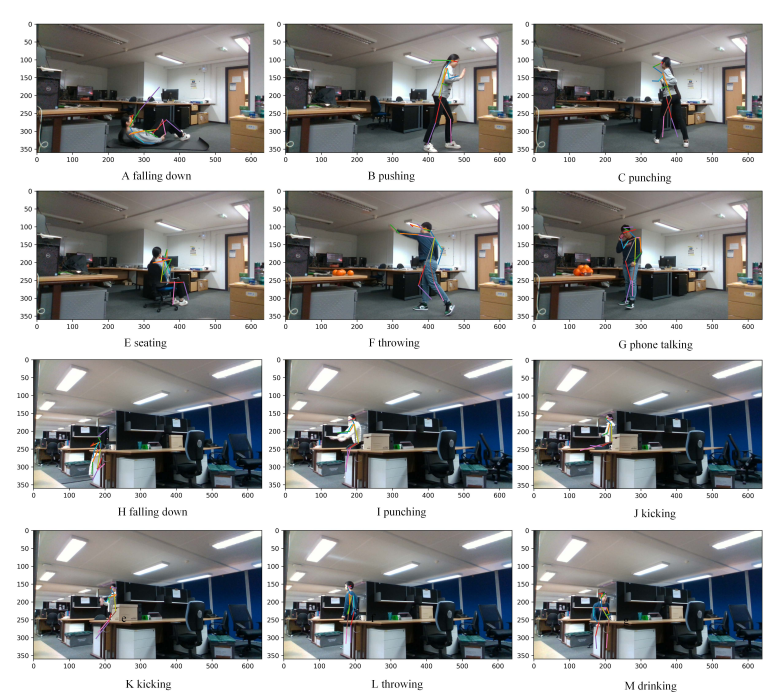
\includegraphics[width=1\textwidth]{./figure/chap 2/7.png}
\caption{The visual skeleton result of the CSI in two scenarios, where A-G are without occlusion scene, and H-M are partial occlusion scene.}
\label{Fig 2.7}
\end{figure}

 \textbf{Limitations:}

\begin{itemize}
\item The number of participants was very small. 
\item The baseline SVM model performed better than their proposed WiNN model.
\end{itemize}

\chapter{THEORETICAL OVERVIEW}
 \label{Chapter 3}
 \lhead{Chapter 3. \emph{Theoretical Overview}}

This chapter provides a theoretical overview of the project as well as specifications for different hardware tools and technologies that are employed.

\section{Hardware Specification}
We use two esp32(ESP-WROOM32) microcontrollers one as a transmitter, and one as a receiver. The features of the device are given below \cite{espDocs}:

\begin{easylist}
 \ListProperties(Style1*=\bfseries,Numbers2=l, Mark1={}, Mark2={)},Indent2=2em)
@ Processors
@@ CPU: Xtensa dual-core (or single-core) 32-bit LX6 microprocessor, operating at 160 or 240 MHz and performing at up to 600 DMIPS
@@ Ultra-low power (ULP) co-processor
@ Memory: 320 KiB RAM, 448 KiB ROM
@ Wireless connectivity:
@@ Wi-Fi: 802.11 b/g/n
@@ Bluetooth: v4.2 BR/EDR and BLE (shares the radio with Wi-Fi)
@ Peripheral interfaces:
@@ 34 × programmable GPIOs
@@ 12-bit SAR ADC up to 18 channels
@@ 2 × 8-bit DACs
@@ 10 × touch sensors (capacitive sensing GPIOs)
@@ 4 × SPI
@@ 2 × I²S interfaces
@@ 2 × I²C interfaces
@@ 3 × UART
@@ SD/SDIO/CE-ATA/MMC/eMMC host controller
@@ SDIO/SPI slave controller
@@ Ethernet MAC interface with dedicated DMA and planned IEEE 1588 Precision Time Protocol support[4]
@@ CAN bus 2.0
@@ Infrared remote controller (TX/RX, up to 8 channels)
@@ Motor PWM
@@ LED PWM (up to 16 channels)
@@ Hall effect sensor
@@ Ultra low power analog preamplifier
@Security:
@@IEEE 802.11 standard security features all supported, including WPA, WPA2, WPA3 (depending on   version)[5] and WLAN Authentication and Privacy Infrastructure (WAPI)
@@     Secure boot
@@     Flash encryption
@@     1024-bit OTP, up to 768-bit for customers
@@     Cryptographic hardware acceleration: AES, SHA-2, RSA, elliptic curve cryptography (ECC), random number generator (RNG)
@Power management:
@@     Internal low-dropout regulator
@@     Individual power domain for RTC
@@     5 $\mu$A deep sleep current
@@     Wake up from GPIO interrupt, timer, ADC measurements, capacitive touch sensor interrupt

\end{easylist}

\begin{figure}[H]
\centering
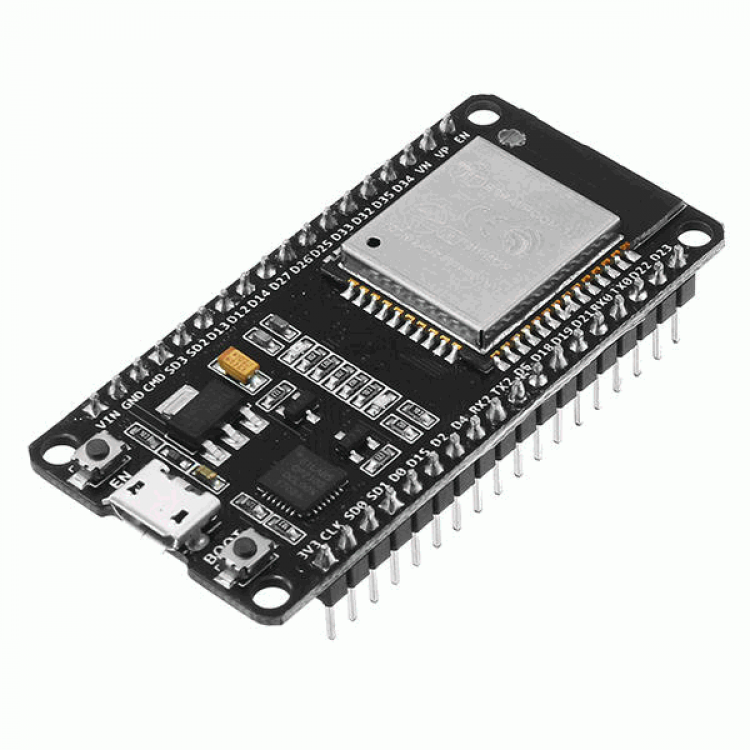
\includegraphics[width=0.7\textwidth]{./figure/chap 3/1.png}
\caption{ A esp32 microcontroller}
\label{Fig 3.1}
\end{figure}

\begin{figure}[H]
\centering
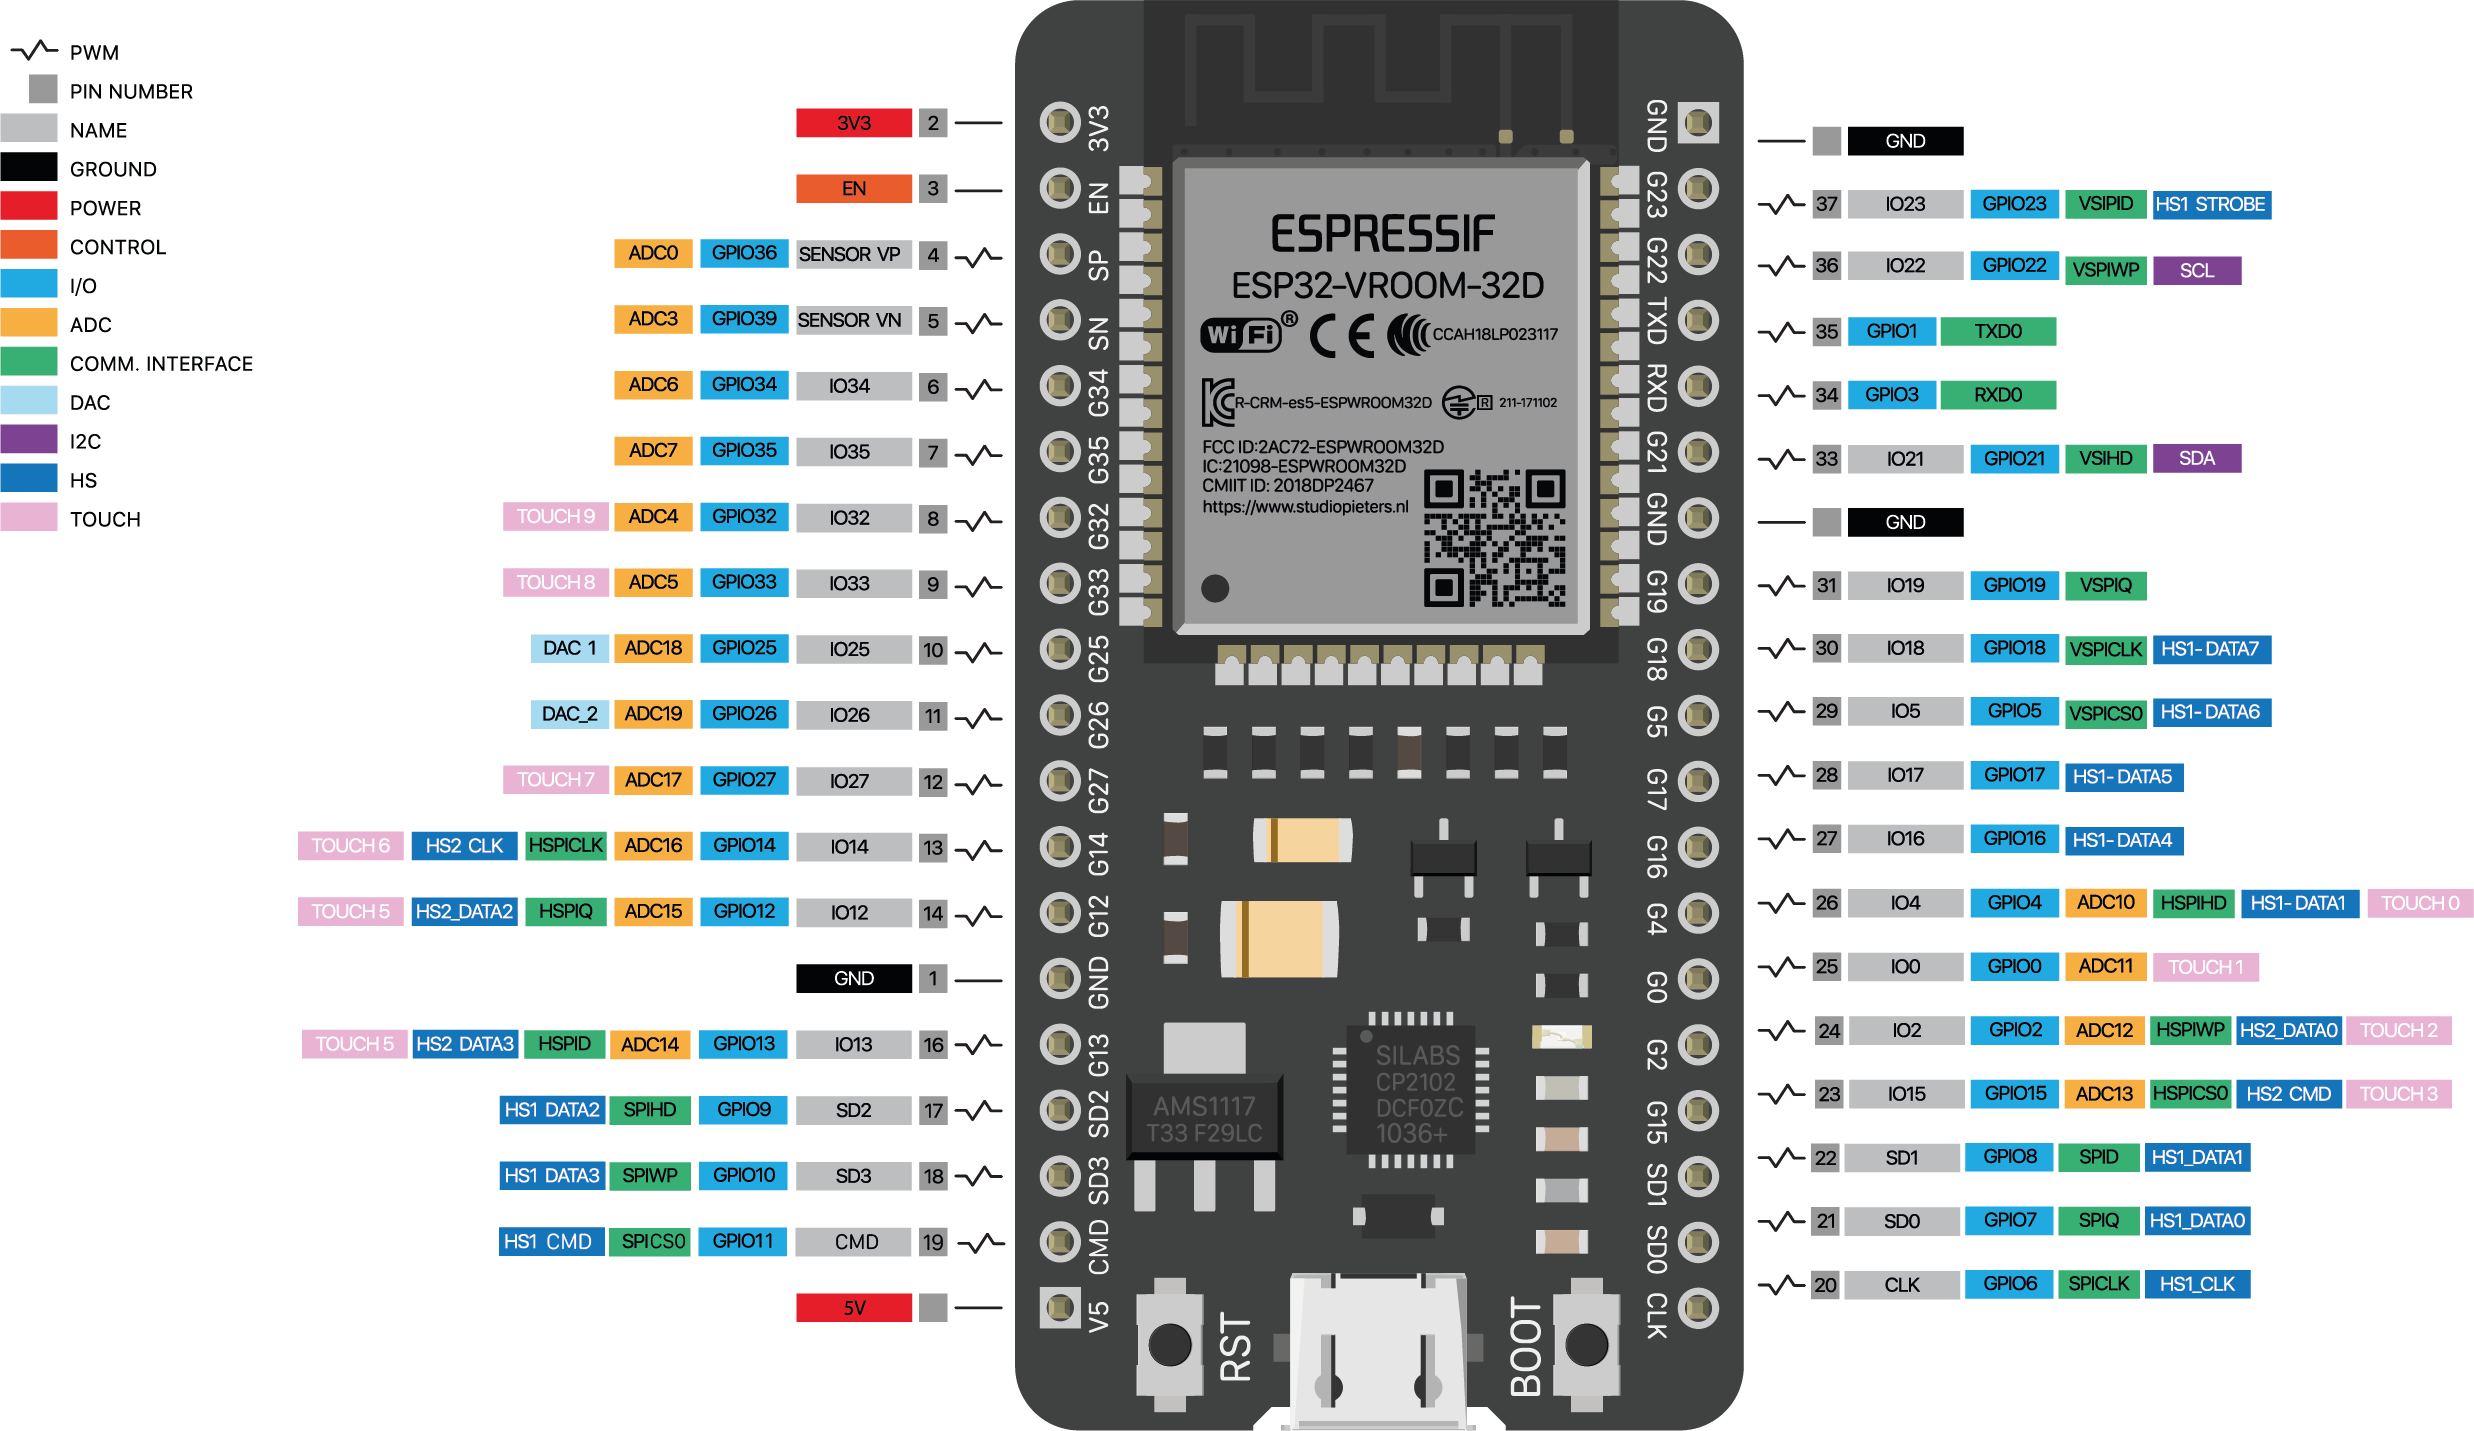
\includegraphics[width=0.7\textwidth]{./figure/chap 3/2.png}
\caption{Pinout diagram of esp32 microcontroller}
\label{Fig 3.2}
\end{figure}

The signal specification for esp32 microconroller is given below:
\begin{itemize}

\item    Bandwidth: 20 MHz
\item    Antenna: 1 RX and 1 TX
\item    Protocol: 802.11n
\item    Modulation: OFDM (16 QAM)
\item    Subcarrier Number:  64
\item    Sampling Rate:  3.9 Hz
\item    Average RSSI: -77 dBm
\item    Guard Interval: 800 ns (MCS Index: 4)
\item    Technologies: MIMO, Frame Aggregation

\end{itemize}

The advantages of using esp32 are:
\begin{itemize}
\item esp32 can function as a stand-alone system or as a slave device to a host MCU, eliminating communication stack overhead on the primary application CPU.
\item Through its SPI / SDIO or I2C / UART interfaces, the esp32 may communicate with other systems to provide Wi-Fi and Bluetooth capability.
\item esp32 has a low-power processor designed for mobile devices, wearable electronics, and IoT applications. It uses a combination of proprietary software to achieve ultra-low power consumption.
\item esp32 is highly-integrated with in-built antenna switches, RF balun, power amplifier, low-noise receive amplifier, filters, and power management modules.
\end{itemize}

In summary, esp32 is ideal for our project because is a power-efficient device that is capable of using wifi communication, is easily integrable with other systems, and has a fair amount of computing power.


\section{Wi-Fi}
In this project, we exploited the capability of Wi-Fi technology to implement fall detection. Wi-Fi, vastly used in high-speed internet access and wireless communication, is a set of protocols governed by IEEE 802.11 standards \cite{7786995}. IEEE 802.11 is part of the local area network (LAN) technical standards and specifies the set of protocols for implementing wireless local area network (WLAN) computer communication. These standards are maintained by the Institute of Electrical and Electronics Engineers (IEEE). Though the first edition of these standards was released in 1997, continuous development is being made and new standards are coming with more capabilities to meet the ever-increasing demand for high-speed wireless communication. The most notable standards of IEEE 802.11 are 802.11a, 802.11b, 802.11g, 802.11n, 802.11ac, and 802.11ax.

\subsection{802.11a}
This was the first standard to use the 5 GHz band for Wi-Fi which might seem to be ahead of its time. But because of the higher frequency, its coverage area was much lower than the traditional 2.4 GHz band and suffered much from interference problem. That is why 802.11a was not so popular compared to its 2.4 GHz counterpart even though it had a higher data rate and went obsolete quickly. But the main contribution of this standard was the introduction of Orthogonal Frequency-Division Multiplexing (OFDM) which improved the data transmission drastically. OFDM is based on the concept of orthogonal subcarriers with minimal interference that makes it possible to cope with severe channel conditions without complex equalization filters. OFDM is described in detail later in this section. 802.11a uses 52 subcarriers in OFDM, of which 48 subcarriers are used for data transmission and the rest 4 subcarriers are used as pilot subcarriers.

\subsection{802.11b}
802.11b was the first widely accepted standard of Wi-Fi. Both 802.11a and 802.11b were released in 1999, with a major difference between them. Unlike 802.11a, 802.11b uses 2.4 GHz band. The 2.4 GHz band was not as crowded as today and offered higher coverage and the capability to withstand interference. These advantages made 802.11b popular despite having a much lower data rate (up to 5.5 Mbit/s). This standard is still in use in some legacy devices.

\subsection{802.11g}
Introduced in 2003, 802.11g was a mixture of the previous two standards. It operated in the 2.4 GHz band like 802.11b and utilizes the same OFDM-based transmission scheme as 802.11a. This technical change gave a burst increase in the data rate which could go up to 54 Mbit/s. 802.11g also uses a total of 52 subcarriers with a carrier separation of 0.3125 MHz. There are 14 partially overlapping channels each of which has a separation of 20 or 25 MHz.

\subsection{802.11n}
This standard is also known as Wi-Fi Generation 4 (Wi-Fi 4). It includes several new technologies that increased the capability of Wi-Fi further. The most notable additions to this standard are:
\begin{itemize}
    \item Multiple Input Multiple Output (MIMO)
    \item Frame aggregation
    \item WiFi Beamforming (Optional)
    \item 40 MHz channel bandwidth
    \item Security enhancement
\end{itemize}
MIMO technology is capable of conducting simultaneous data transmission over multiple antennas. Frame aggregation allows sending two or more frames in a single transmission. Beamforming improves the user experience by focusing the Wi-Fi beams in the user's direction. Thus these new features along with OFDM increased the data rate from 72 Mbit/s to 600 Mvit/s. 802.11n has support for the 2.4 GHz band and optionally for the 5 GHz band. Most Wi-Fi-enabled devices are still using this standard today.

\subsection{Newer standards}
After 802.11n, a few major standards have come out that have increased the data rate, reliability, and security further. 802.11ac (Wi-Fi 5) is currently spreading in the consumer community which uses only the 5 GHz band. It introduced a few new features, such as Multi-User MIMO (MU-MIMO), wider 80 MHz and 160 MHz channels, and Beamforming. 

802.11ax (Wi-Fi 6E) is the most recently approved standard adopted in 202 which uses three bands: 2.4 GHz, 5 GHz, and 6 GHz. The data rate can vary from 600 Mbit/s to 9608 Mbit/s. Currently, the development is being made for 802.11be standard or Wi-Fi 7 which will provide even more data rate.

The hardware used in our proposed method, esp32 uses the popular IEEE 802.11n standard. It currently has the largest user base and can utilize several recent technologies including OFDM, MIMO, and frame aggregation.

\subsection{OFDM}

Orthogonal Frequency-Division Multiplexing (OFDM) is a sort of digital transmission and a way of encoding digital data on multiple carrier frequencies that is used in telecommunications. OFDM is a widely used wideband digital communication technique, with applications including digital television and audio broadcasting, DSL internet access, wireless networks, power line networks, and 4G/5G mobile communications.\cite{1}
The capacity of OFDM to cope with severe channel conditions without the use of sophisticated equalization filters is its fundamental benefit over single-carrier methods. Because OFDM uses numerous slowly modulated narrowband signals rather than a single rapidly modulated wideband signal, channel equalization is simpler. This mechanism also makes it easier to design single frequency networks (SFNs), in which multiple adjacent transmitters send the same signal at the same frequency at the same time, because the signals from multiple distant transmitters can be constructively recombined, avoiding the interference that a traditional single-carrier system would face.

\begin{figure}[H]
\centering
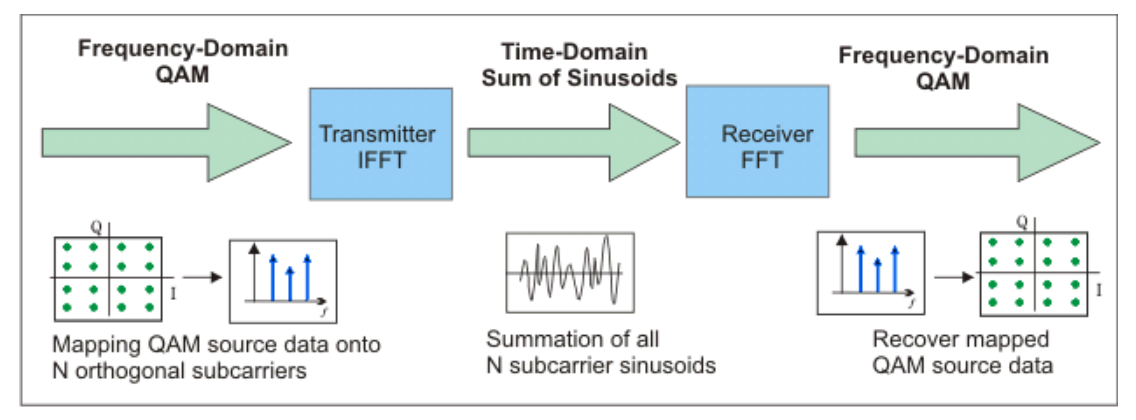
\includegraphics[width=1.0\textwidth]{./figure/chap 3/ofdm.png}
\caption{Block Diagram of Simplified OFDM  System}
\label{Fig 3.3}
\end{figure}

\subsection{MIMO}

Multiple-Input MIMO (Many-Input, Multiple-Output) is a wireless technology that uses multiple transmitters and receivers to carry more data at once. MIMO is supported by all 802.11n wireless equipment. The technology enables 802.11n to achieve faster rates than goods that do not have 802.11n.\cite{mimo}
MIMO must be supported by the station (mobile device) or the access point (AP) to be implemented. Both the station and the access point must support MIMO for the best performance and range.
Multipath, a natural radio-wave phenomenon, is used in MIMO technology. Multipath occurs when transmitted data bounces off walls, ceilings, and other obstacles, arriving at the receiving antenna numerous times at slightly varying angles and times. Multipath created interference and hindered wireless communications in the past. MIMO technology with multipath combines numerous, smart transmitters and receivers with an extra spatial dimension to improve performance and range.
By allowing antennas to mix data streams arriving from diverse paths and at different times, MIMO boosts the signal-capturing power of receivers. Smart antennas make use of spatial diversity technology, which makes use of unused antennas. When the number of antennas outnumbers the number of spatial streams, the antennas can boost receiver variety and range.\cite{CORVAJA2008288}

\begin{figure}[H]
\centering
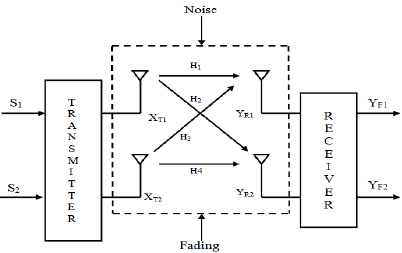
\includegraphics[width=1.0\textwidth]{./figure/chap 3/mimo.png}
\caption{Block Diagram of MIMO System}
\label{Fig 3.4}
\end{figure}


\section{Signals used for analysis}
Activity recognition using Wi-Fi data is not a completely new domain. Older methods of human activity recognition used Received Signal Strength Indication (RSSI) signal. But recently with the development in WLAN fields, newer standards starting from 802.11g can provide Channel State Information (CSI) signal too. In our proposed method, we utilized both signals to classify human activity more accurately. Here is an overview of these signals.

\subsection{RSSI}
The RSSI is a measurement of the signal's power at the moment it reaches the receiver. Signal energy diminishes with distance, according to signal propagation models and experiments. As a result, RSSI is frequently used in conjunction with multilateration algorithms to estimate position. When impediments are present in the region of interest, RSSI suffers from several drawbacks. RSSI values are distributed randomly and its correlation with the distance is not strong due to Multipath and shadowing fading effects. RSSI values are comparatively coarse information which is the result of averaging the amplitudes of all incoming signals to the receiver. These drawbacks lead to poor localization performance using RSSI \cite{Wang2016}. This problem can be solved by using rich channel information from different subcarriers.

\subsection{CSI}
In IEEE 802.11 a/g/n/ac/ax networks, data transmission and reception is done using OFDM. As discussed earlier, OFDM uses a number of orthogonal subcarriers to transmit data in multiple spatial paths. While a transmitting packet is in the medium, it is subjected to different obstructions, such as, fading, scattering and power loss. As the subcarriers follow different spatial paths, these obstructions affect each subcarrier differently. Thus this physical layer information specific to each subcarrier is known as Channel State Information (CSI). CSI is an overall depiction of the channel state that includes scattering, fading, and multipath effects in the signal's propagation. In contrast to the received power strength provided by RSSI, CSI statistics provide more information about the channel degradation effects that the signal suffers due to its granularity of sub-carrier frequencies and vector representation. Data is sent using MIMO and OFDM systems.

In narrow-band flat fading channel, a MIMO system is represented by:
\begin{equation}
    y_i = Hx_i + N_i
\end{equation}
where $y_i$ and $x_i$ are the received and the transmitted signal
vectors respectively, $H$ denotes the channel matrix which contains the CSI information and $N_i$ is the noise vector. To estimate the channel matrix $H$, a known training sequence or the pilot sequence is transmitted and channel response $H$ is measured at the receiver side. If the pilot sequence is expressed by $x_1, x_2, x_3, ... , x_n$, the received can be represented by: 
\begin{equation}
    Y = [y_1 + y_2 + ... + y_n] = HX + N
\end{equation}
Thus the channel matric can be determined by: 
\begin{equation}
    \hat{H} = \frac{Y}{X}
\end{equation}
For any MIMO system of $n \times m$ dimension, $H$ can be shown in matrix form:
\begin{equation}
    H_i = \begin{bmatrix}
    h_{11} & h_{12} & h_{13} & ... & h_{1m}\\ 
    h_{21} & h_{22} & h_{23} & ... & h_{2m}\\ 
    ... & ... & ... & ... & ... \\
    h_{n1} & h_{n2} & h_{n3} & ... & h_{nm}\\ 
    \end{bmatrix}
\end{equation}
where $i$ is the subcarrier index and $h_nm$ is a complex number representing the amplitude and phase information of Channel State Information (CSI).

\section{Machine Learning}
In the 1950s, a branch of artificial intelligence known as machine learning was discovered and developed. The earliest machine learning techniques date back to the 1950s, however there have been very few notable studies and advancements in this field. However, this field of study underwent a resurgence in the 1990s and has continued to this day. Future advancements in this field of study are expected. The complexity of analyzing and interpreting the data, which is continually expanding, is what has led to this development. The foundation of machine learning is the idea that, with the help of this growing data, the best model for the new data may be found among the old data. As a result, research into machine learning will continue along with the growth in data.\cite{mlArticle}
The actions performed by computers, which are based on an algorithm and follow specific procedures, have no margin for error. In some circumstances, computers make judgments based on the current sample data, which is different from commands that are created to produce an outcome depending on an input. In some circumstances, computers may err in their decision-making just like people do. Putting it another way, machine learning is the process of giving computers the capacity to learn from data and experience just like a human brain.\cite{jetol457046}The primary goal of machine learning is to develop models that can learn from previous data to become better, recognize complicated patterns, and find answers to new problems.\cite{Turk}

\subsection{Machine Learning Categories}
We can divide machine learning approaches in four categories.They are:
\begin{itemize}
    \item Supervised Learning
    \item Unsupervised Learning
    \item Semi-supervised Learning
    \item Reinforced Learning
\end{itemize}

Supervised learning is a technique where the currently available input data is used to arrive at the outcome set. Classification and regression supervised learning are the two categories of supervised learning.
\begin{enumerate}
    \item Classification: Dividing the data into the categories specified in the data set in accordance with their unique characteristics.
    \item Regression: Predicting or drawing conclusions about the other characteristics of the data from the known characteristics.
\end{enumerate}

Unsupervised learning is the technique where the output is not provided while training the model.The algorithms following this technique can be classified into two categories:
\begin{enumerate}
    \item Clustering: When intrinsic groupings in the data are unknown, finding groups of data that are comparable to one another.
    \item Association: Figuring out the links and relationships between the data in the same data collection.
\end{enumerate}

Semi-supervised learning is a method of machine learning that, during training, blends a sizable amount of unlabeled data with a small amount of labeled data. Between supervised learning (with labeled training data) and unsupervised learning is semi-supervised learning (with only labeled training data). It is a unique illustration of poor supervision. Either inductive learning or transductive learning may be referred to as semi-supervised learning.\cite{Zhu071contents}

Reinforcement learning is the challenge that an agent faces when learning behavior through trial-and-error interactions with a dynamic environment. Reinforcement learning differs from supervised learning in that it does not need the presentation of labeled input/output pairings or the explicit correction of suboptimal behaviors. Instead, the emphasis is on striking a balance between exploitation and exploration (of undiscovered territory) (of current knowledge). The benefits of supervised and RL algorithms can be combined with partially supervised RL algorithms.\cite{DBLP:journals/corr/cs-AI-9605103}

\section{Human Activity Recognition}
Human activity recognition is important for interpersonal interactions and human-to-human communication. It is challenging to extract since it contains details about a person's identity, personality, and psychological condition. One of the key research topics in the fields of computer vision and machine learning is the human capacity for activity recognition. This research has led to the need for multiple activity detection systems in numerous applications, such as video surveillance systems, human-computer interaction, and robotics for characterizing human behavior. Most of the work in human activity recognition assumes a figure-centric scene of an uncluttered background, where the actor is free to perform an activity. The development of a fully automated human activity recognition system, capable of classifying a person’s activities with low error, is a challenging task due to problems, such as background clutter, partial occlusion, changes in scale, viewpoint, lighting and appearance, and frame resolution.\cite{10.3389/frobt.2015.00028}

To solve these issues, a task is needed that combines three elements: (i) background subtraction, in which the system tries to distinguish between the foreground's changing or moving objects and the background's parts;\cite{1032799}\cite{s19061352} (ii) human tracking, in which the system tracks a person's motion over time;\cite{10.1016/j.patcog.2013.10.019} and (iii) human action and object detection, in which the system can localize a person's activity.\cite{Ganetal}

\begin{figure}[H]
\centering
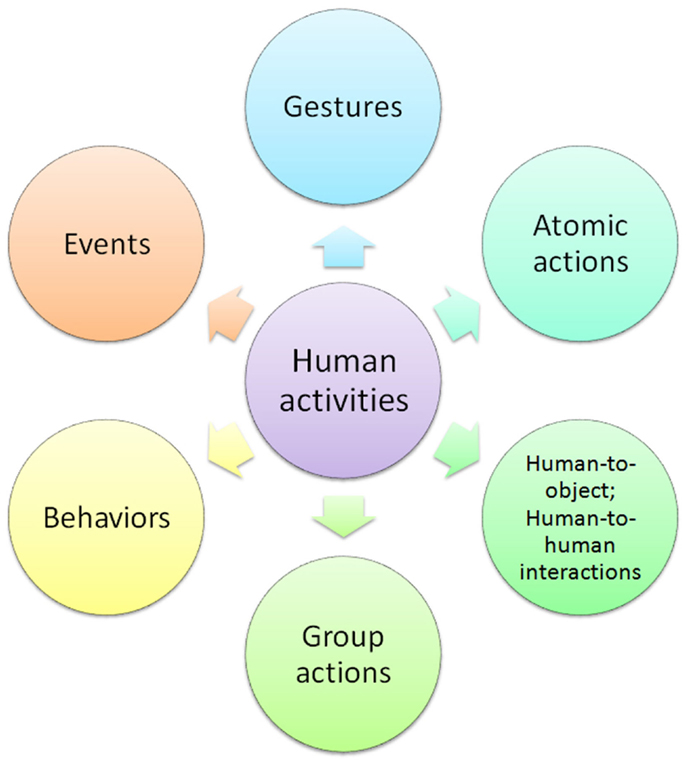
\includegraphics[width=0.7\textwidth]{./figure/chap 3/3.jpg}
\caption{Decomposition of human activities.}
\label{Fig 3.5}
\end{figure}

\section{Classification Algorithms}
Classification algorithm is a Supervised Learning technique that is used to categorize new observations based on training data. In classification, a program makes use of the dataset or observations that are provided to learn how to categorize new observations into various classes or groups. Some algorithms are discussed here:
\begin{itemize}
    \item SVM: Support vector machines (SVMs) are a group of supervised learning techniques for classifying data, performing regression analysis, and identifying outliers. Support vector machines have the following benefits: efficient in high-dimensional environments. Still useful in situations where the number of dimensions exceeds the number of samples.\cite{svm}
    \item Random Forest: A large number of decision trees are built during the training phase of the random forests or random decision forests ensemble learning approach, which is used for classification, regression, and other tasks. The class that the majority of the trees chose is the output of the random forest for classification problems. Decision trees tend to overfit their training set, and random decision forests correct for this. Although they frequently outperform decision trees, gradient boosted trees are more accurate than random forests.\cite{rforest}
    \item Extra Trees Classifier: In essence, it involves dividing a tree node while severely randomizing the choice of attribute and cut-point. In the worst situation, it creates completely random trees, whose architectures are independent of the learning sample's output values. By selecting the right parameter, the strength of the randomization can be adjusted to the particulars of the problem. The algorithm's biggest advantage, aside from accuracy, is computational speed.\cite{etclassifier}
        \begin{figure}[H]
        \centering
        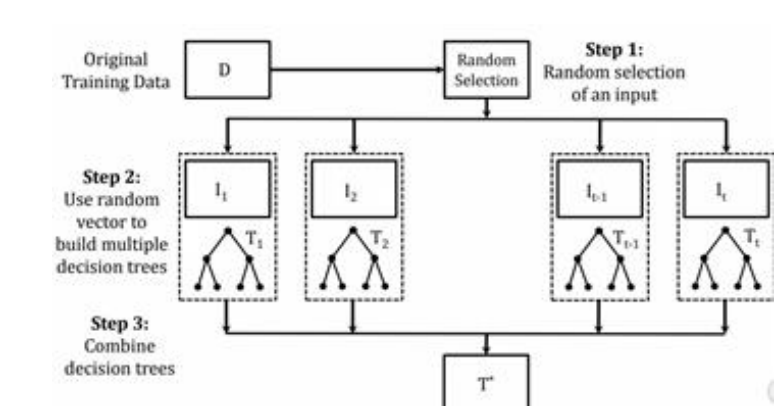
\includegraphics[width=0.7\textwidth]{./figure/chap 3/4.png}
        \caption{Visual Representation of Extra Trees Classifier.}
        \label{Fig 3.6}
        \end{figure}

    
    \item Artificial Neural Network(ANN): Artificial neural network is based on research into the brain and nervous system, as seen in Fig. 1. Although they employ a condensed set of biological brain system ideas, these networks mimic biological neural networks. Particularly, ANN models mimic the electrical activity of the nerve system and brain. Connected to other processing elements are processing elements (sometimes called neurodes or perceptrons). The neurodes are typically organized in layers or vectors, with the output of one layer acting as the input for the following layer and maybe other layers.\cite{ann}
        \begin{figure}[H]
        \centering
        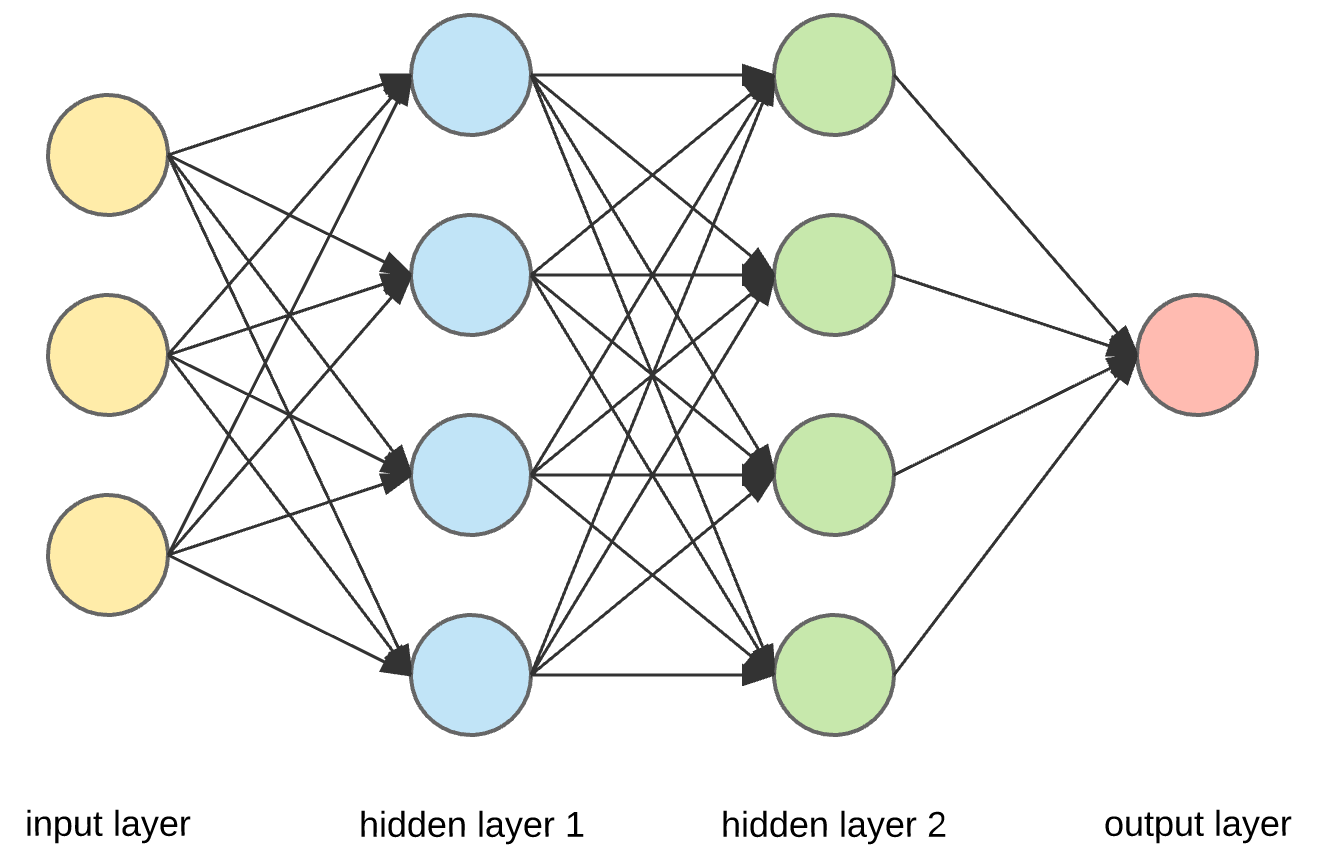
\includegraphics[width=0.7\textwidth]{./figure/chap 3/5.png}
        \caption{Visual Representation of an Artificial Neural Network.}
        \label{Fig 3.6}
        \end{figure}

\end{itemize}








\chapter{METHODOLOGY}
 \label{Chapter 4}
 \lhead{Chapter 4. \emph{Methodology}}

In this chapter, we will discuss the implementation of our proposed system. At first, we will describe the hardware setup used for collecting user data. Different aspects of the dataset were mentioned in the next subsection. Later, we discussed how we extracted, processed, calibrated, and denoised the raw data and made them usable for our model. Finally, a brief overview of our proposed model and approach is given.

\section{Hardware Setup}
The main hardware we used for this system is a pair of ESP32 MCU manufactured by espressif. The specific model of the used hardware module is ESP32-WROOM-32E. This is an ESP32-D0WD-based module with Wi-Fi 802.11 b/g/n and Bluetooth LE 4.2 connectivity and a dual-core processor. Traditional research on Wi-Fi-based human activity recognition uses Intel 5300 or Atheros 9390 Network Interface Card (NIC) of a laptop computer \cite{10.1145/3310194, 9264288, 9060143, 8873550, 10.1145/2789168.2790093} which is not a realistic choice for practical use because each node is a computer. The device we used is small, low-cost, programmable, and deployment-friendly and the whole system needs only one computer to process the data. 

For our experiment, we need to send CSI data from one ESP32 device to another. But ESP32 does not transmit CSI data with the initially provided firmware. So, a customized firmware by Espressif Systems \cite{esp-csi} is flashed to the devices to enable the transmission of CSI data. CSI data can be received using three ways:
\begin{enumerate}

\item \textbf{Get router CSI data:} In this process, a router is used to send CSI data to the ESP32. Firstly, the ESP32 device sends a Ping request to the router with an empty ICMP packet. The router acknowledges the request by sending a Ping Replay back to the requesting device. The CSI information is transmitted with the Ping Replay. One disadvantage of this process is that we need an extra router device and set it up separately to send CSI data.

\begin{figure}[H]
\centering
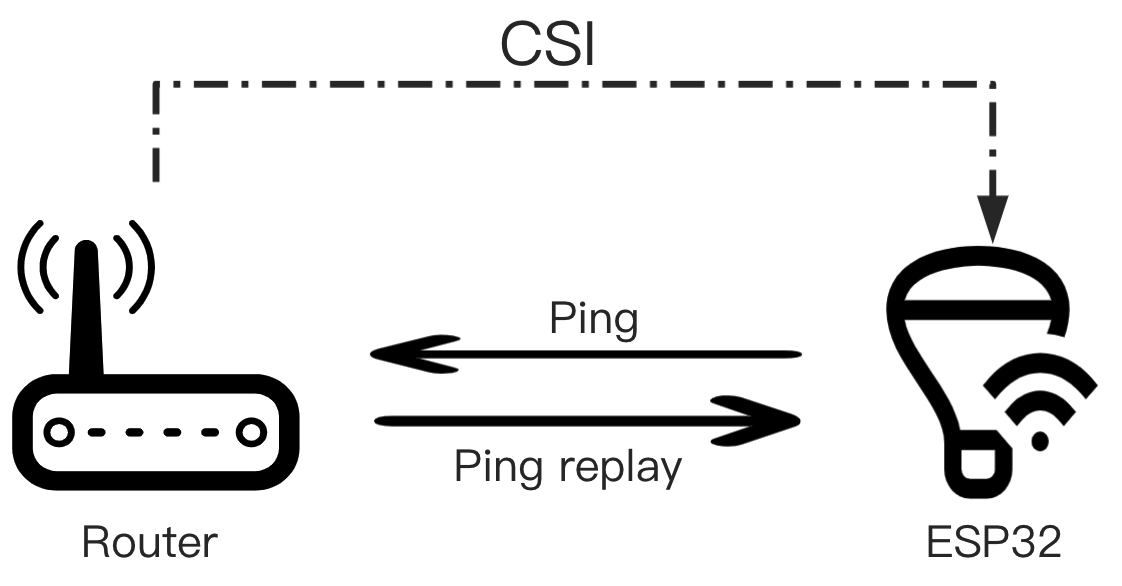
\includegraphics[width=1.0\textwidth]{./figure/chap 4/get_router_csi.png}
\caption{Get CSI data of the router}
\label{Fig 4.1}
\end{figure}

\item \textbf{Get device CSI data using router:} To implement this method, we need two ESP32 devices. ESP32 A and B both send Ping packets to the router, and ESP32 A receives the CSI information carried in the Ping Replay returned by ESP32 B. In this method, the CSI data is passed from ESP32 A to ESP32 B using an intermediate router. This intermediate connection may reduce the packet receiving rate of the system.

\begin{figure}[H]
\centering
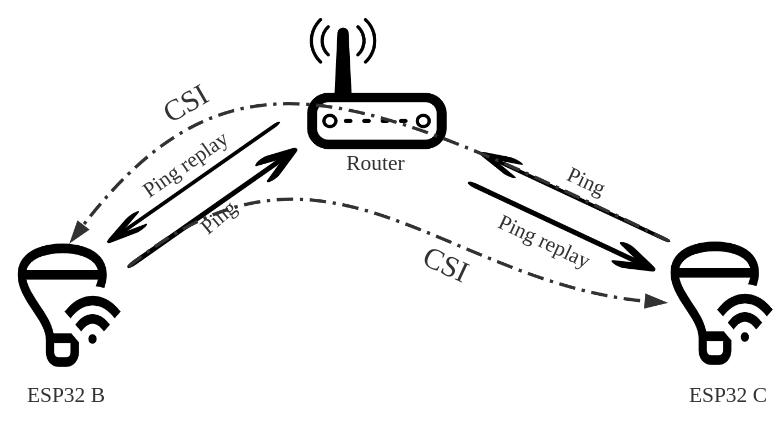
\includegraphics[width=1.0\textwidth]{./figure/chap 4/get_device_csi.png}
\caption{Get CSI data between devices using a router}
\label{Fig 4.2}
\end{figure}

\item \textbf{Get device CSI data using broadcasting:} In this method, one ESP32 device acts as a transmitting device and all other devices are receiving device. The transmitting ESP32 A sends CSI data using broadcasting. This method has the highest detection accuracy and reliability and does not require any router device. 

\begin{figure}[H]
\centering
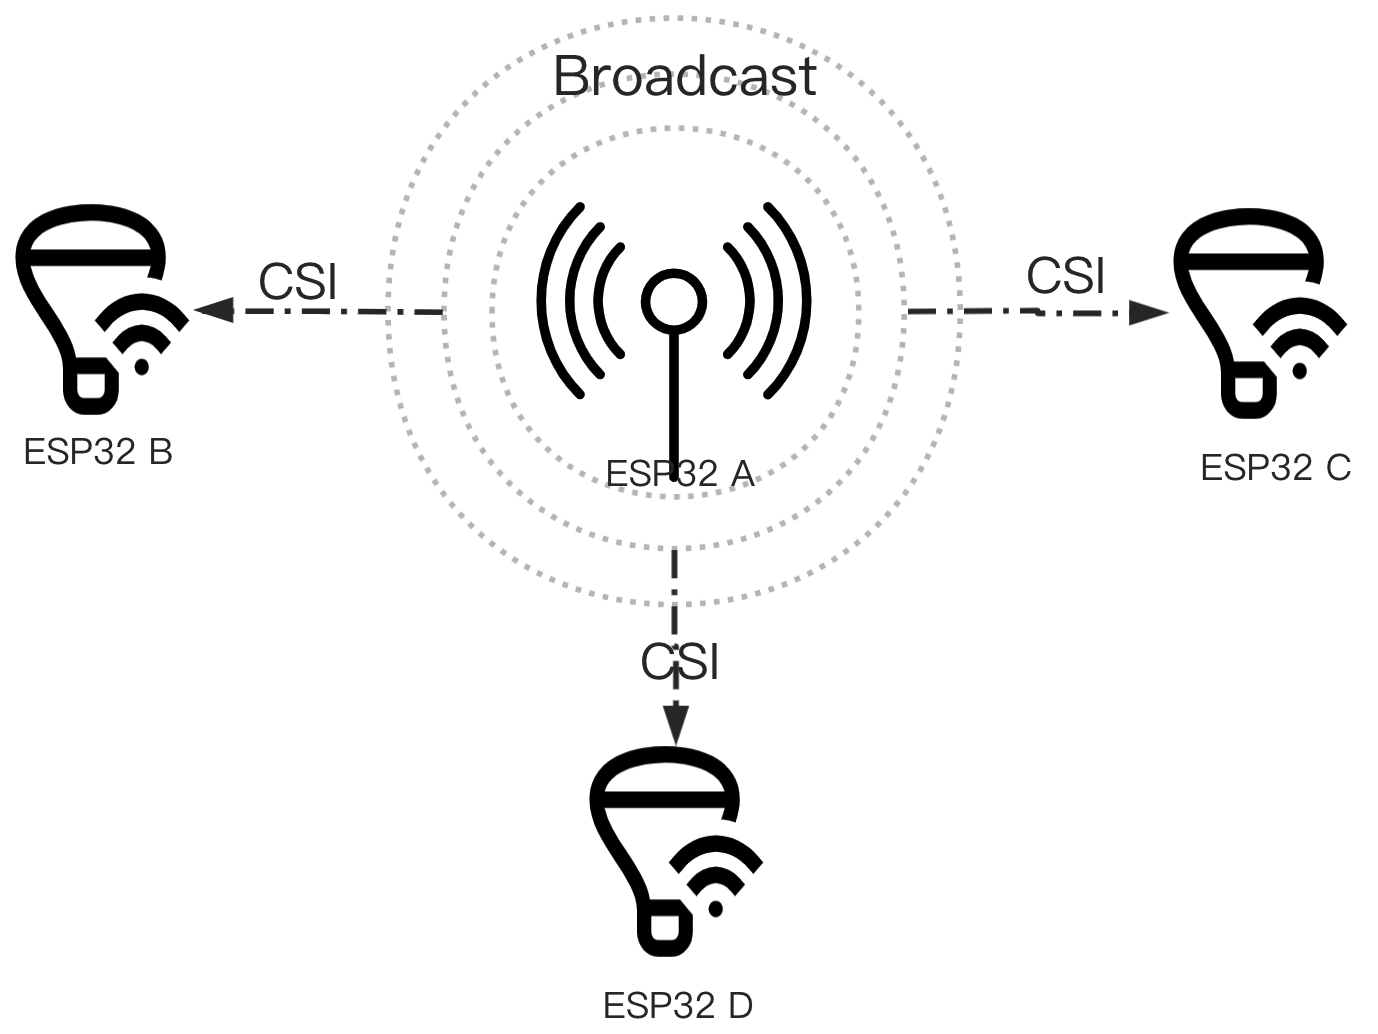
\includegraphics[width=1.0\textwidth]{./figure/chap 4/get_broadcast_csi.png}
\caption{Get CSI data using a broadcasting ESP32}
\label{Fig 4.3}
\end{figure}

\end{enumerate}

As we focus on reliability and accuracy, we choose the third method by making one ESP32 device a broadcaster and the other a receiver. We added an extra layer of security by specifying the Media Access Control (MAC) address of the receiving ESP32. As a result, if the receiving device is in the coverage area of the transmitting device, it gets CSI data automatically from the transmitting device. No overhead is required here.

        \begin{figure}[H]
        \centering
        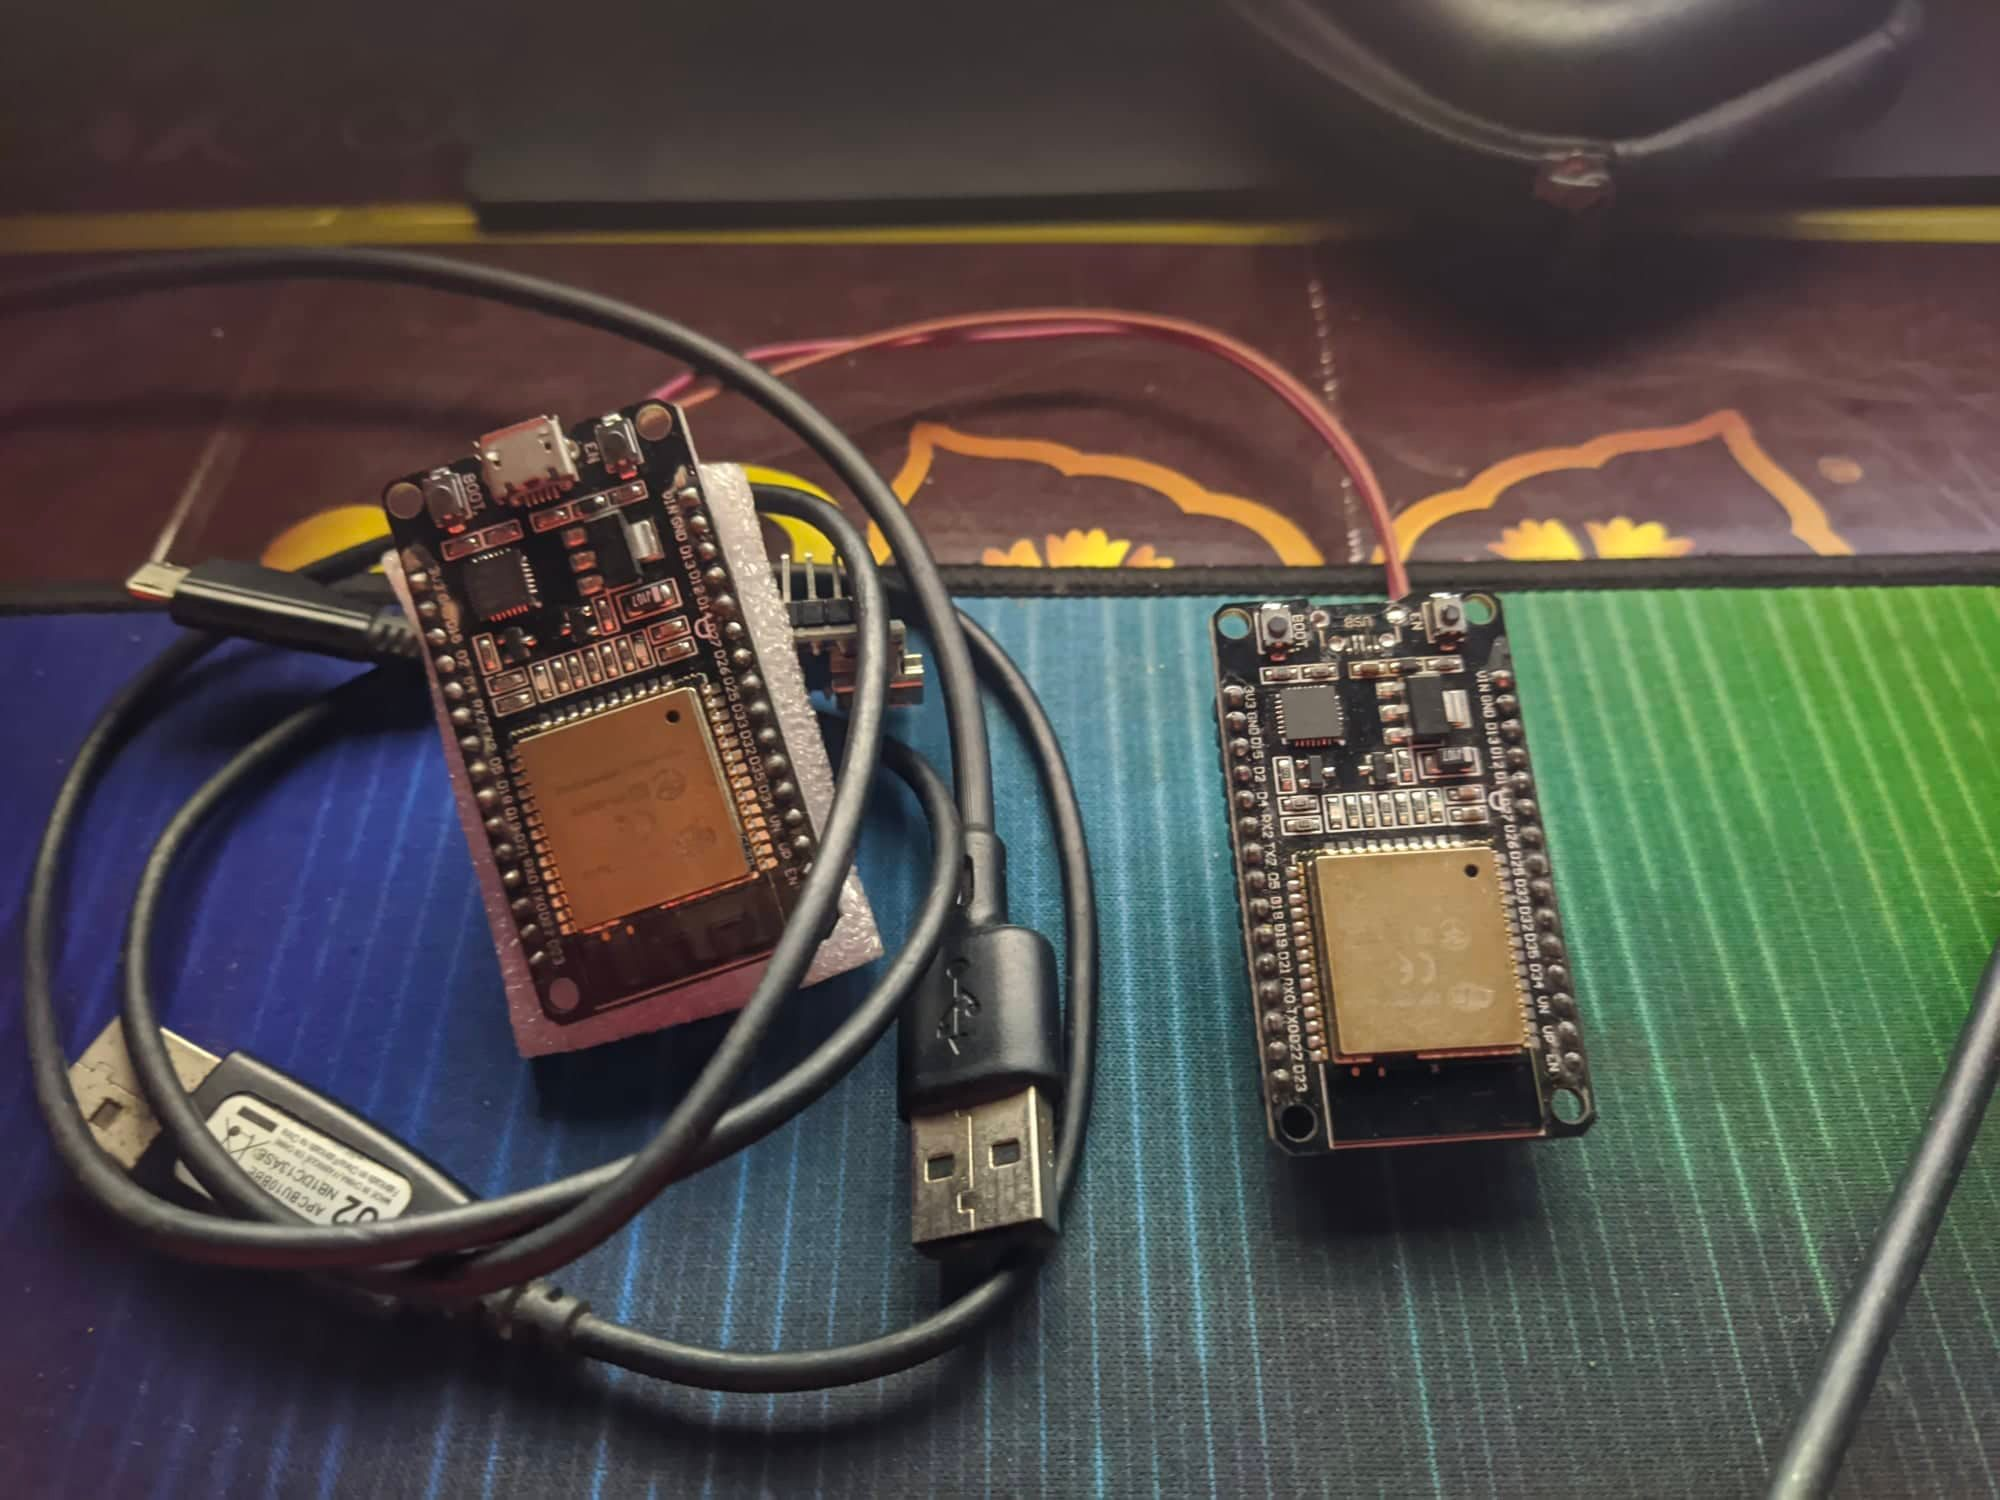
\includegraphics[width=1\textwidth, trim={0 0 0 6cm}, clip]{./figure/chap 4/myesp.jpg}
        \caption{ESP32 devices used in the project}
        \label{Fig 4.4}
        \end{figure}


Each ESP32-WROOM-32E module has one built-in PCB antenna that can transmit or receive data. It is also possible to connect any external antenna with 50 $\Omega$ resistance. In this experiment, we restricted our study to the built-in PCB antenna. We used two ESP32 modules placed approximately 3.5 meters apart. One of them is used as a transmitting device connected to any power source, and the other as a receiving device connected to a computer to process the data and predict the activity. The space between the devices is kept empty for ensuring the Line-of-Sight (LoS). The subjects are instructed to do the activities in the 3.5 meters $\times$ 3.5 meter area between the transmitting and receiving devices. Because of the movement of the subject, the transmitting packets face multipath fading, scattering, reflection, and power loss. The Channel State Information (CSI) of each packet can be analyzed to find patterns between the transmitting packets using machine learning algorithms and thus recognize the activity performed by the subject.

        \begin{figure}[H]
        \centering
        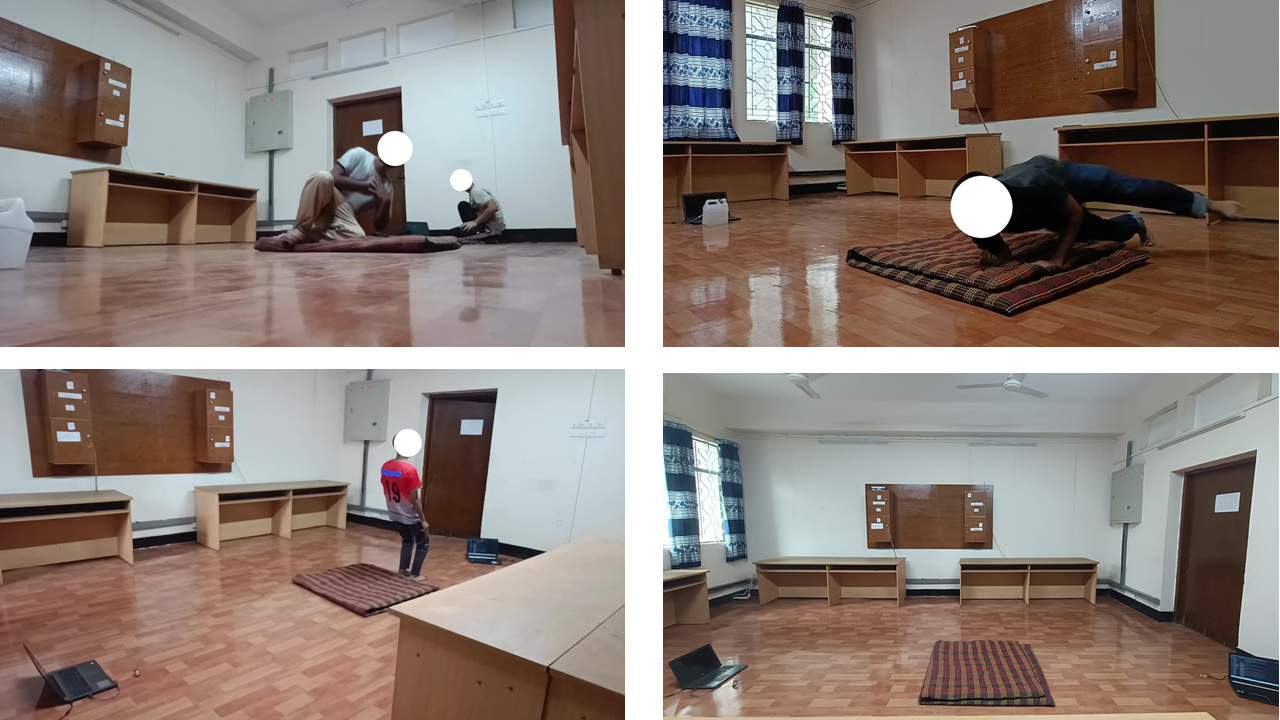
\includegraphics[width=1\textwidth]{./figure/chap 4/dataCollection.png}
        \caption{Data Collection Setup and Data Collection Example}
        \label{Fig 4.5}
        \end{figure}


ESP32-WROOM-32E supports Wi-Fi 802.11 b/g/n standards. For our experiment, we used 802.11n standard that provides support for OFDM, MIMO, frame aggregation, and higher data rate. But ESP32 does not support 5 GHz band and only works with 2.4 GHz band. The ESP32 devices we used in this experiment are configured to send data according to the following specifications:

\begin{table}[H]
\caption{Customized signal specification of ESP32}
\vspace{2mm}
\centering
\begin{tabular}{|l|l|} 
\hline
\multicolumn{1}{|c|}{\textbf{Specification}} & \multicolumn{1}{c|}{\textbf{Value}}                                                             \\ 
\hline
Standard               & IEEE 802.11n   \\
Band                   & 2.4 GHz        \\
Channel                & 20 MHz         \\
MCS index              & 0              \\
Guard interval         & 400 ns         \\
Data rate              & 7.2 Mbit/s     \\
Modulation             & BPSK           \\
Sampling rate          & 100 Hz         \\
Coding rate            & 1/2            \\
Spatial streams        & 1              \\
\hline

\end{tabular}
\label{Table 4.1}
\end{table}


\section{Dataset Description}
The accuracy and effectiveness of any data-driven study depend much on a well-prepared dataset. But there are only a few open datasets available for activity recognition using ESP32 CSI data. But these datasets do not have enough data or provide the activities we need for this system. Hence, we prepared our dataset using the hardware setup stated in the previous section. Wi-Fi CSI data is very sensitive to the outside environment which makes it very hard to collect data in the wild. Even rooms with different arrangements may affect the CSI data differently which may create a problem if a huge amount of data is not taken. For this project, we selected a neat and spacious room with minimum furniture and other things to collect the data. Two ESP32 devices are placed 3.5 meters apart and the activities are performed by different subjects in the area between the two devices. There are a total of 5 activities performed by 13 individual subjects. Each activity segment is recorded for a fixed time window of 4 seconds. This time window is chosen empirically by the type and complexity of the activities. A total of 966 samples of such segments are recorded on different calendar days.

\subsection{Challenges}
ESP32 sends Ping packets with CSI data at a rate of 100 Hz. But due to interference, unavailability of Line of Sight, and other issues, some packets are lost. As a result, though ideally each data segment of 4 seconds should have a total of $ 4 \times 100 = 400$ packets, most of the segments had packets between 300 to 340 due to packet loss.

\begin{figure}[H]
\centering
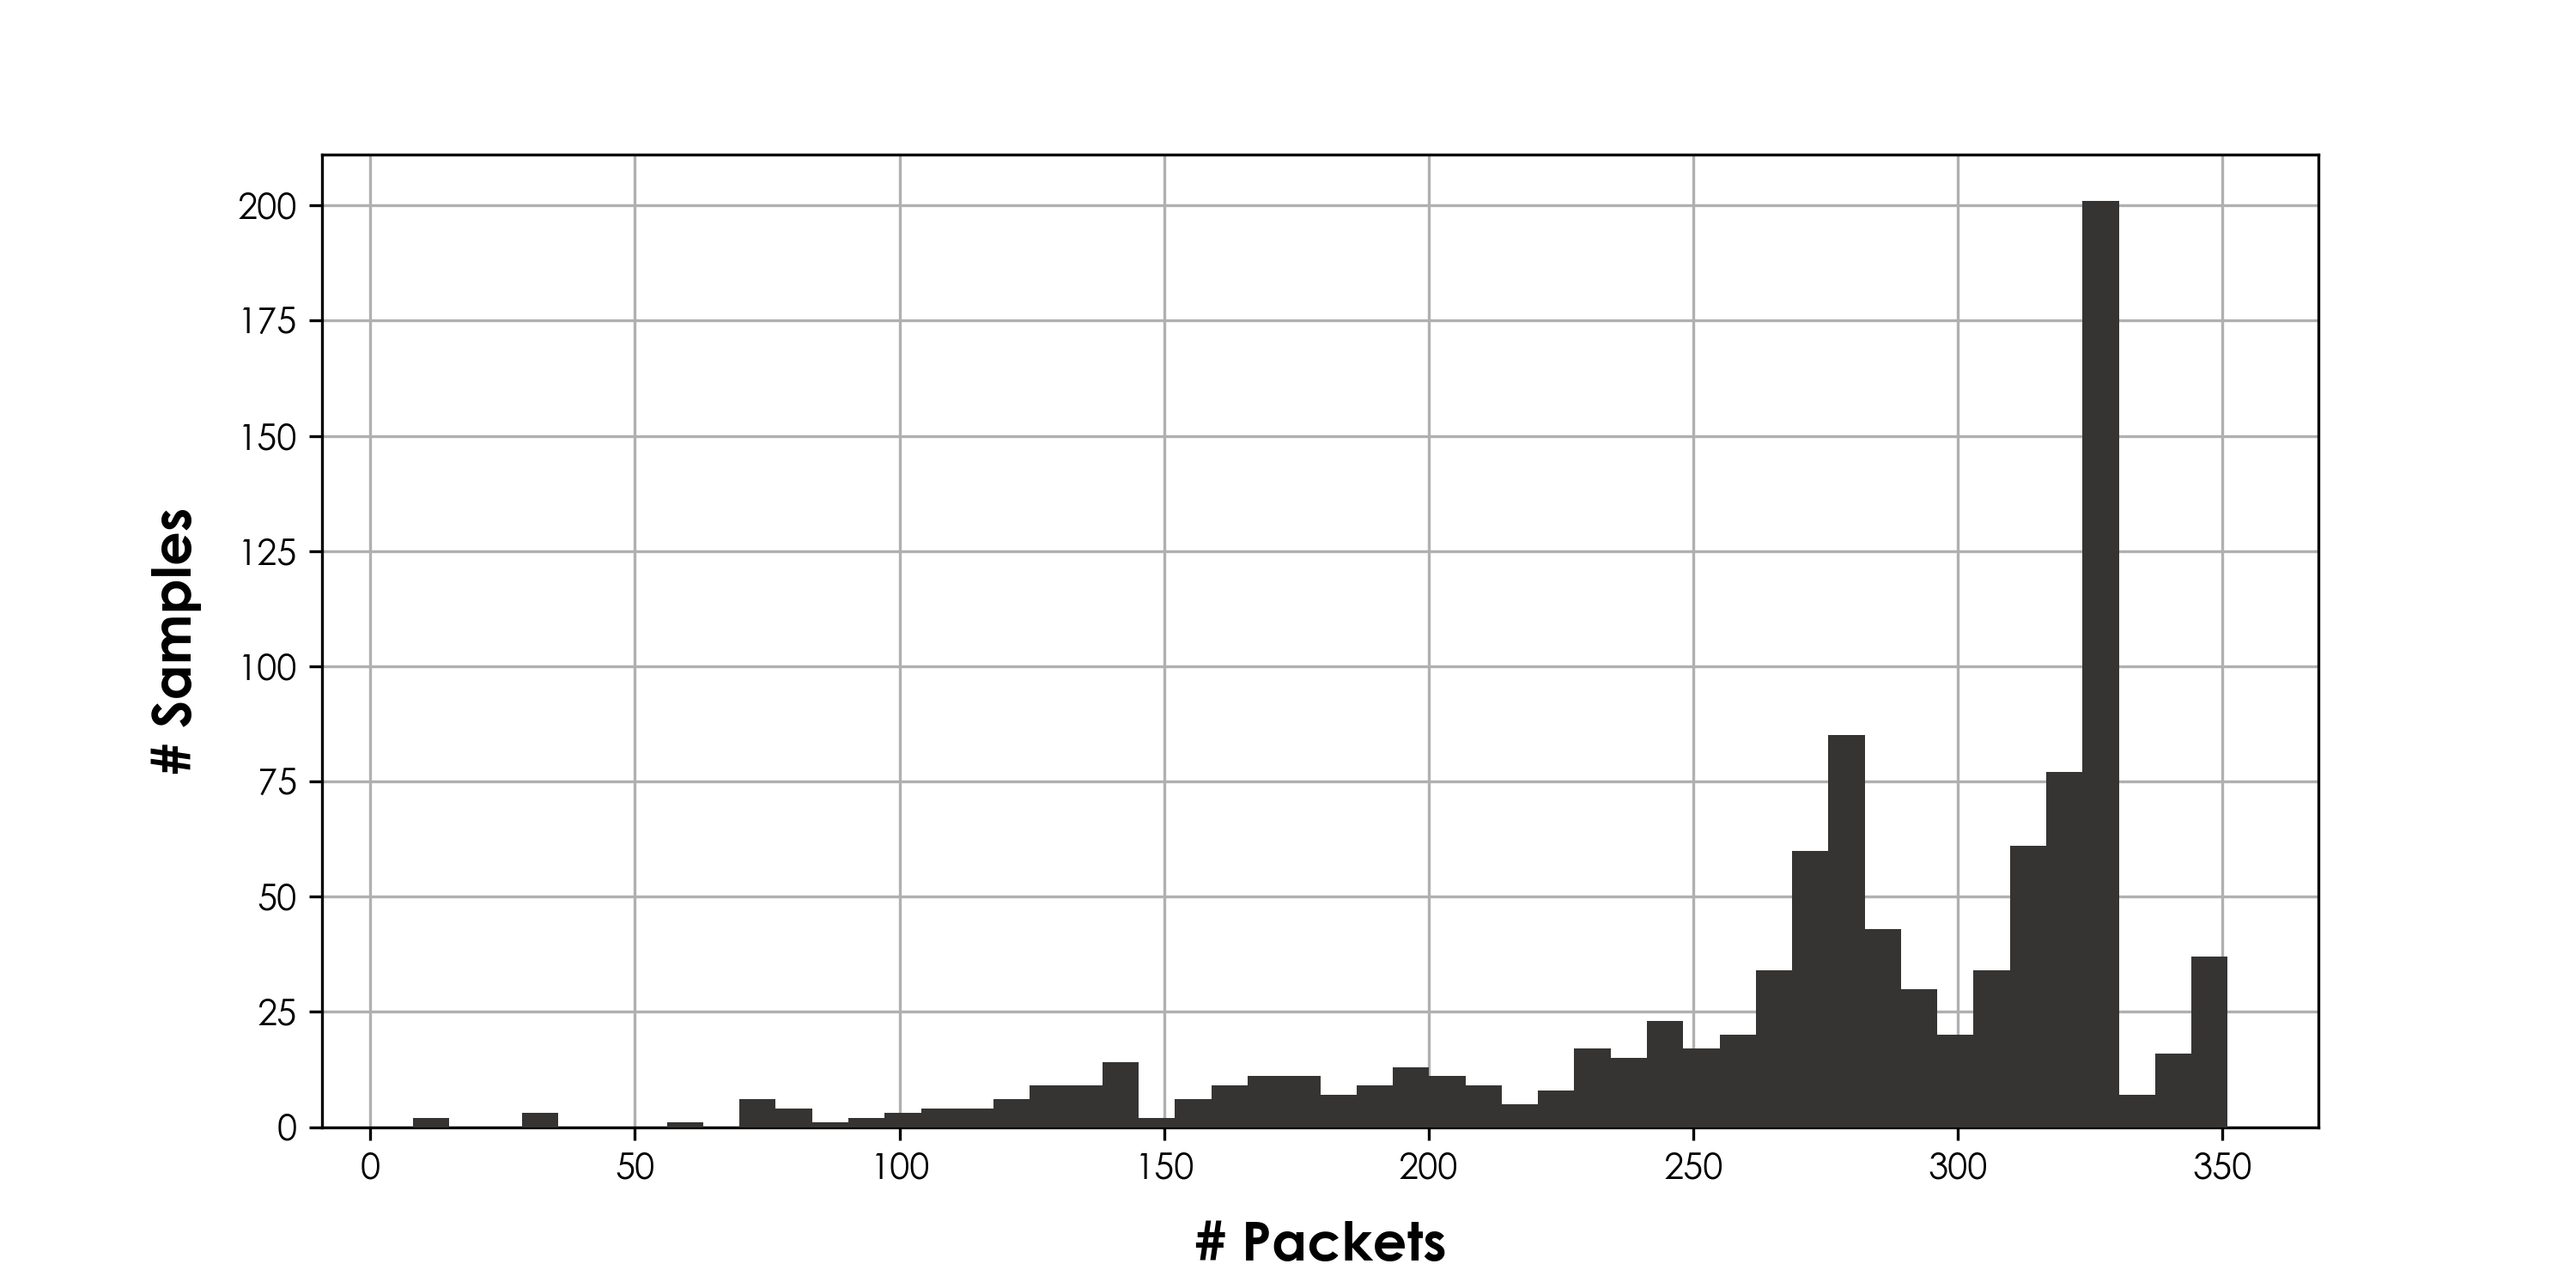
\includegraphics[width=1.0\textwidth]{./figure/chap 4/all_data_sizes.png}
\caption{Distribution of number of packets in all the collected samples}
\label{Fig 4.6}
\end{figure}

The problem here is, some of the data samples had extremely lower number of packets that were not usable in the system. So, we discarded 68 data samples with less than 150 packets. Finally, the remaining 898 data samples were used in the next steps. 

\begin{figure}[H]
\centering
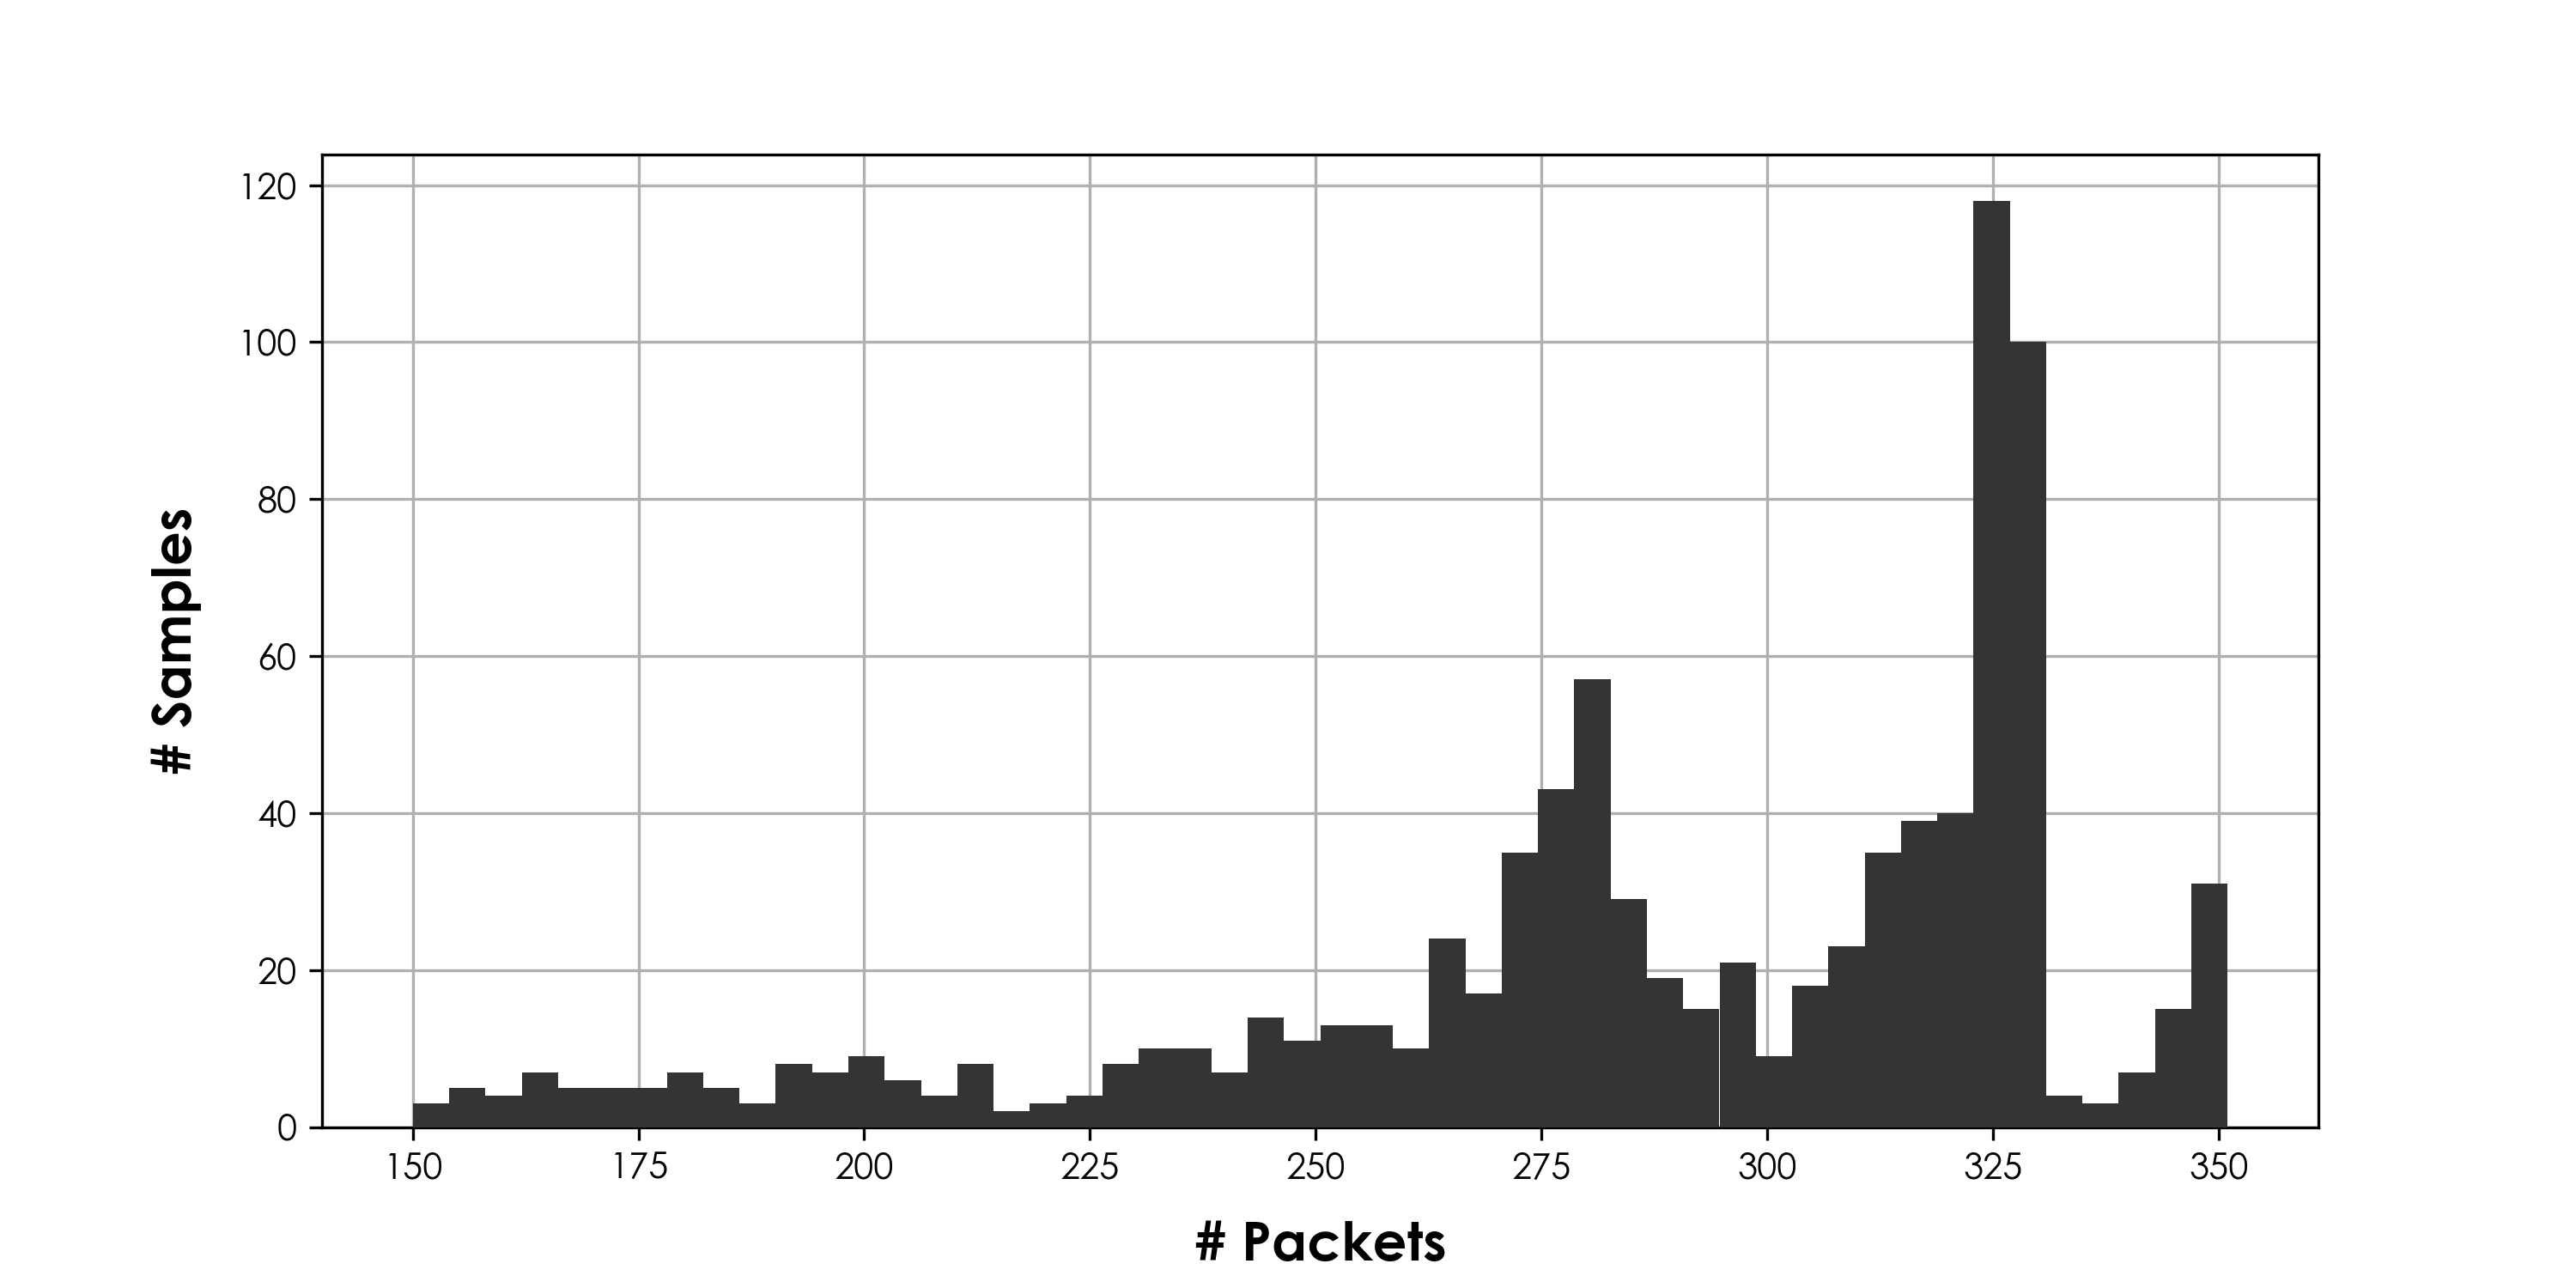
\includegraphics[width=1.0\textwidth]{./figure/chap 4/selected_data_sizes.png}
\caption{Distribution of number of packets in the selected samples}
\label{Fig 4.7}
\end{figure}

\subsection{Activities}
There are a total of 5 activities in this dataset: \emph{Fall}, \emph{Stand}, \emph{Walk}, \emph{Empty Room} and \emph{Presence}. \emph{Fall}, \emph{stand} and \emph{walk} activities are performed by one subject for each sample. For \emph{empty room} activity, no subject was present in the room. For \emph{presence}, a few subjects were present in the room doing various daily activities including gossiping, taking rest, writing, etc. Every activity excluding the \emph{empty room} was done in a different direction and fashion to preserve generality. The number of samples for each of the activity are not the same and is shown below in \ref{Table 4.2}.

\begin{table}[H]
\caption{Number of samples by activity}
\vspace{2mm}
\centering
\begin{tabular}{|l|c|} 
\hline
\multicolumn{1}{|c|}{\textbf{Activity}} & \multicolumn{1}{c|}{\textbf{Number of samples}}                                                      \\ 
\hline
Fall                   & 224            \\
Stand                  & 100            \\
Walk                   & 133            \\
Empty room             & 299            \\
Presence               & 142            \\
\hline
\end{tabular}
\label{Table 4.2}
\end{table}

\begin{figure}[H]
\centering
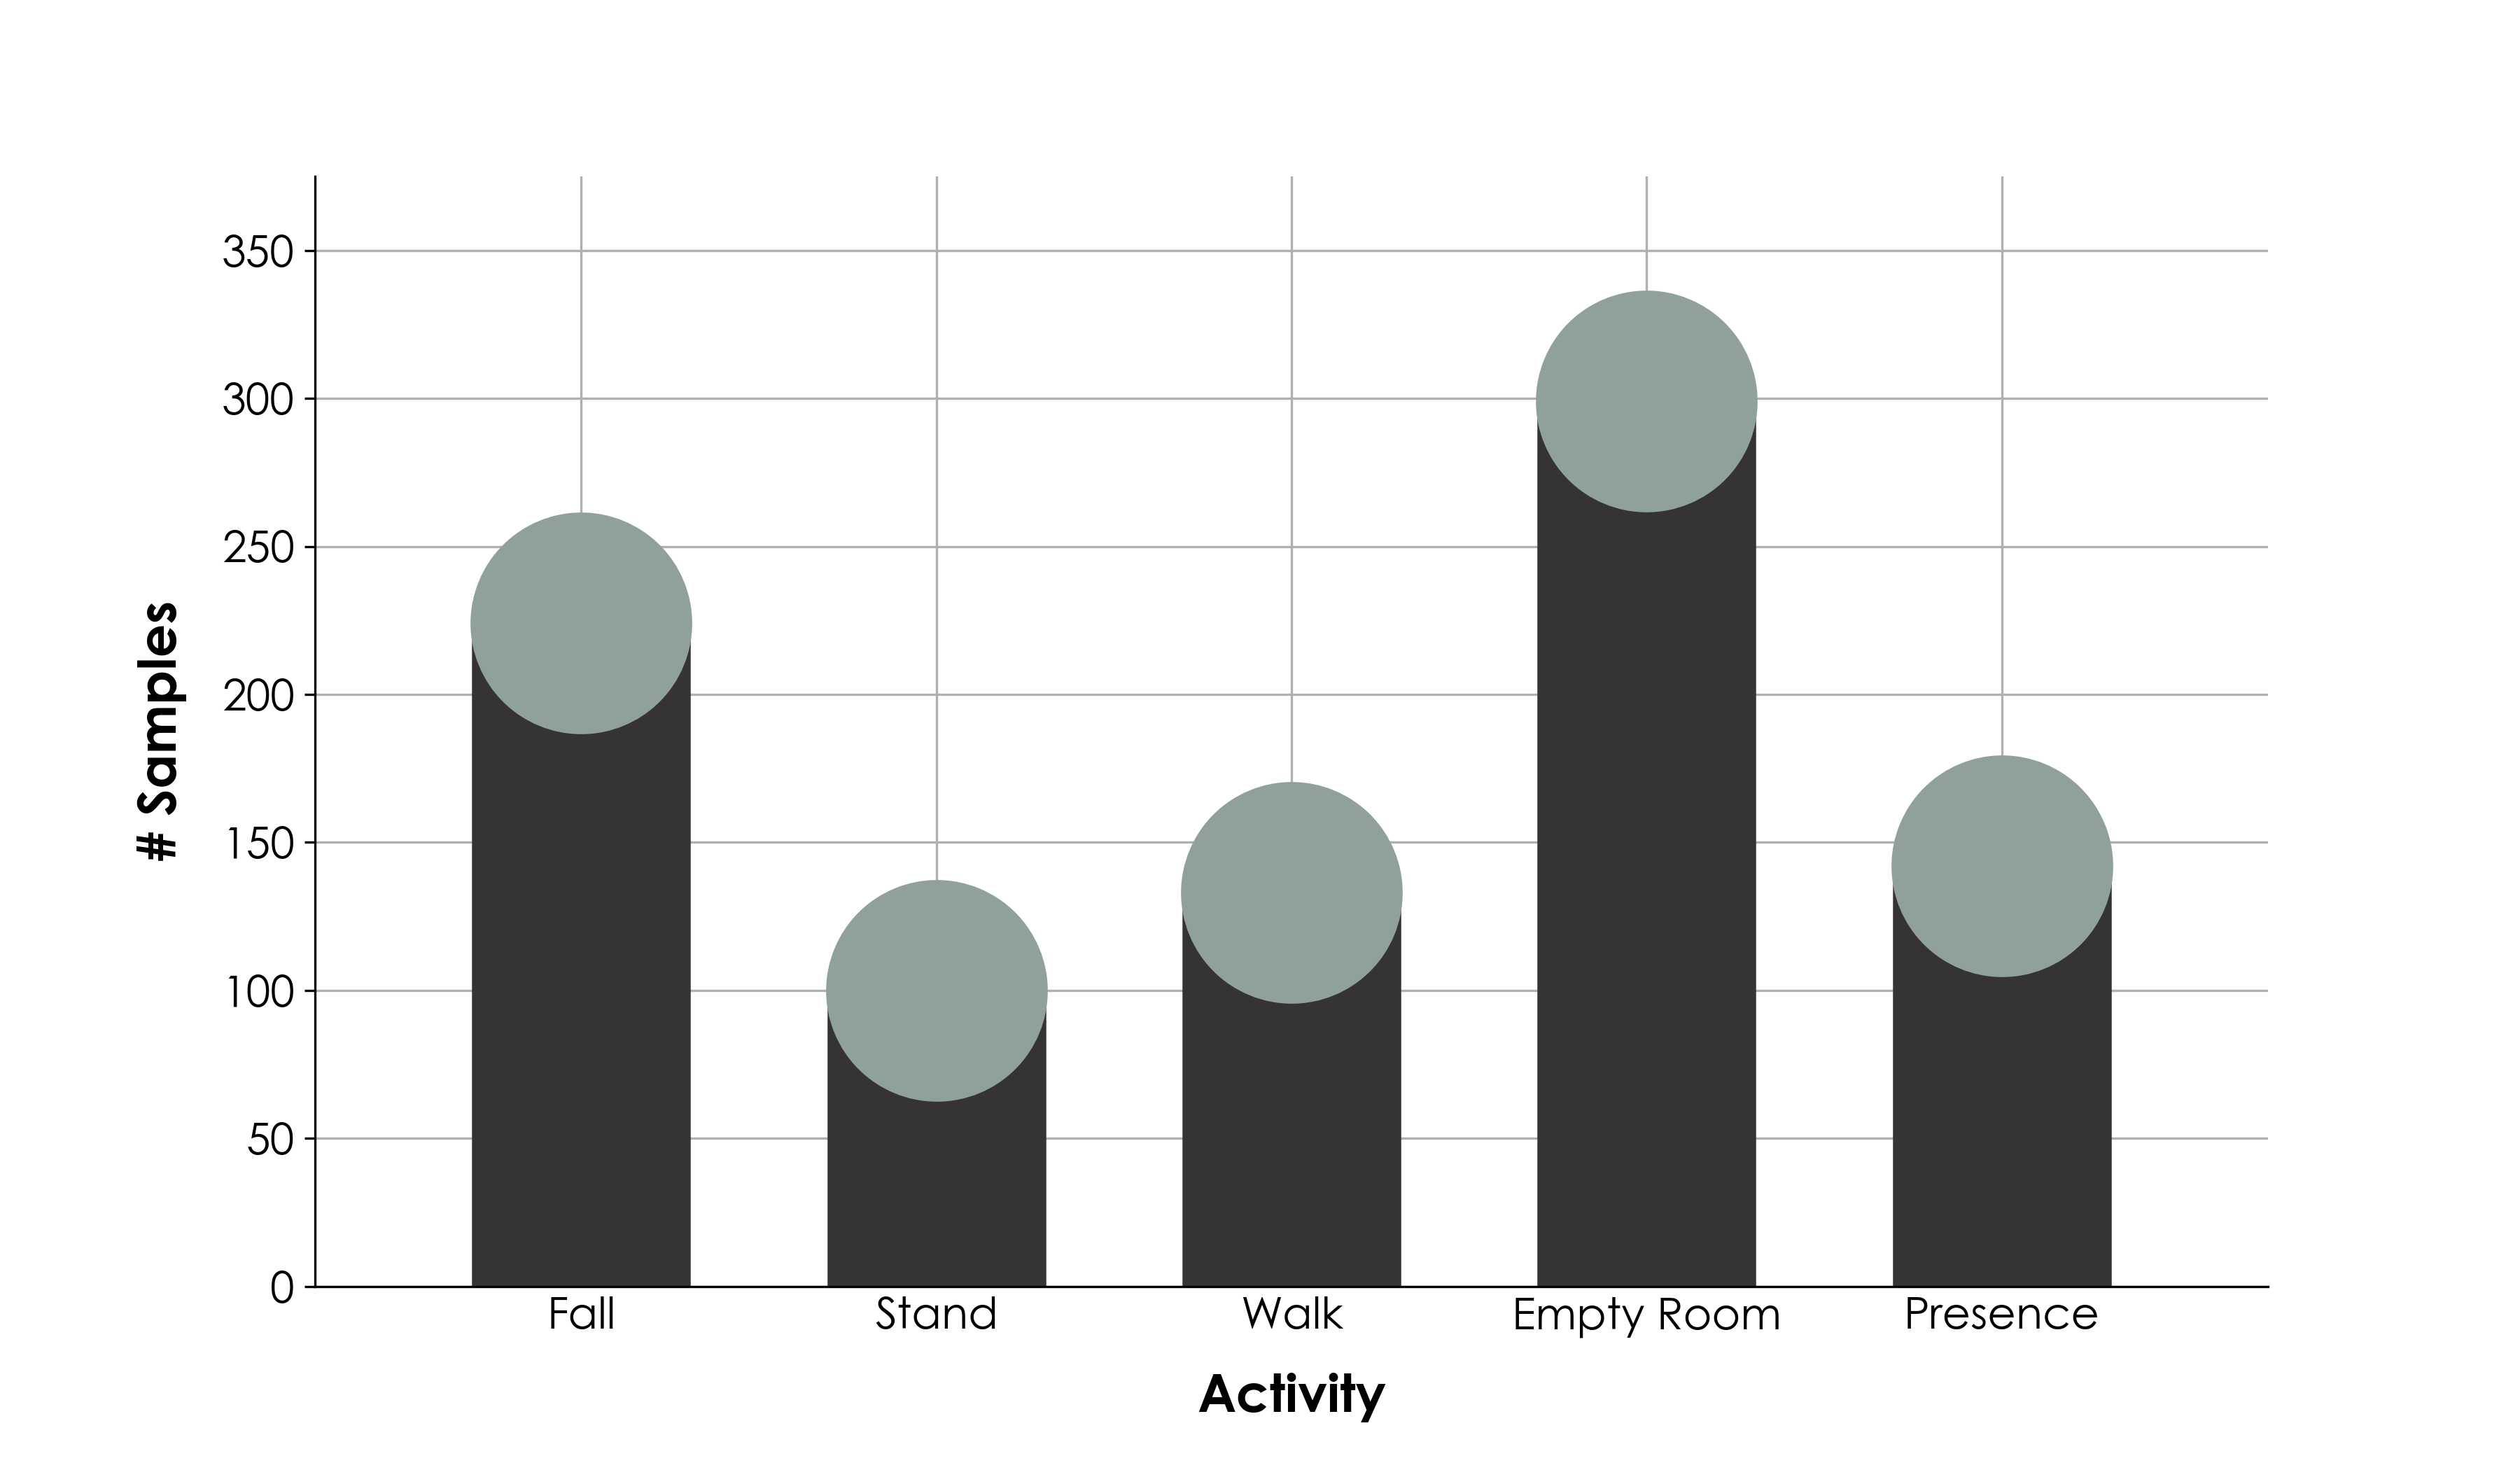
\includegraphics[width=1.0\textwidth]{./figure/chap 4/labelwise_data_counts.png}
\caption{Number of samples by activity}
\label{Fig 4.8}
\end{figure}

Packet size distribution is also different for different types of activities. As subcarriers experience a different level of scattering, reflection, or delay for different types and speeds of movement, packet loss will also be different. For example, \emph{stand} activity involves a very small amount of movement, but there should be a much higher level of movement in \emph{fall} activity. This difference in movement causes a difference in packet loss and segment size as illustrated in \ref{Fig 4.9}.

\begin{figure}[H]
\centering
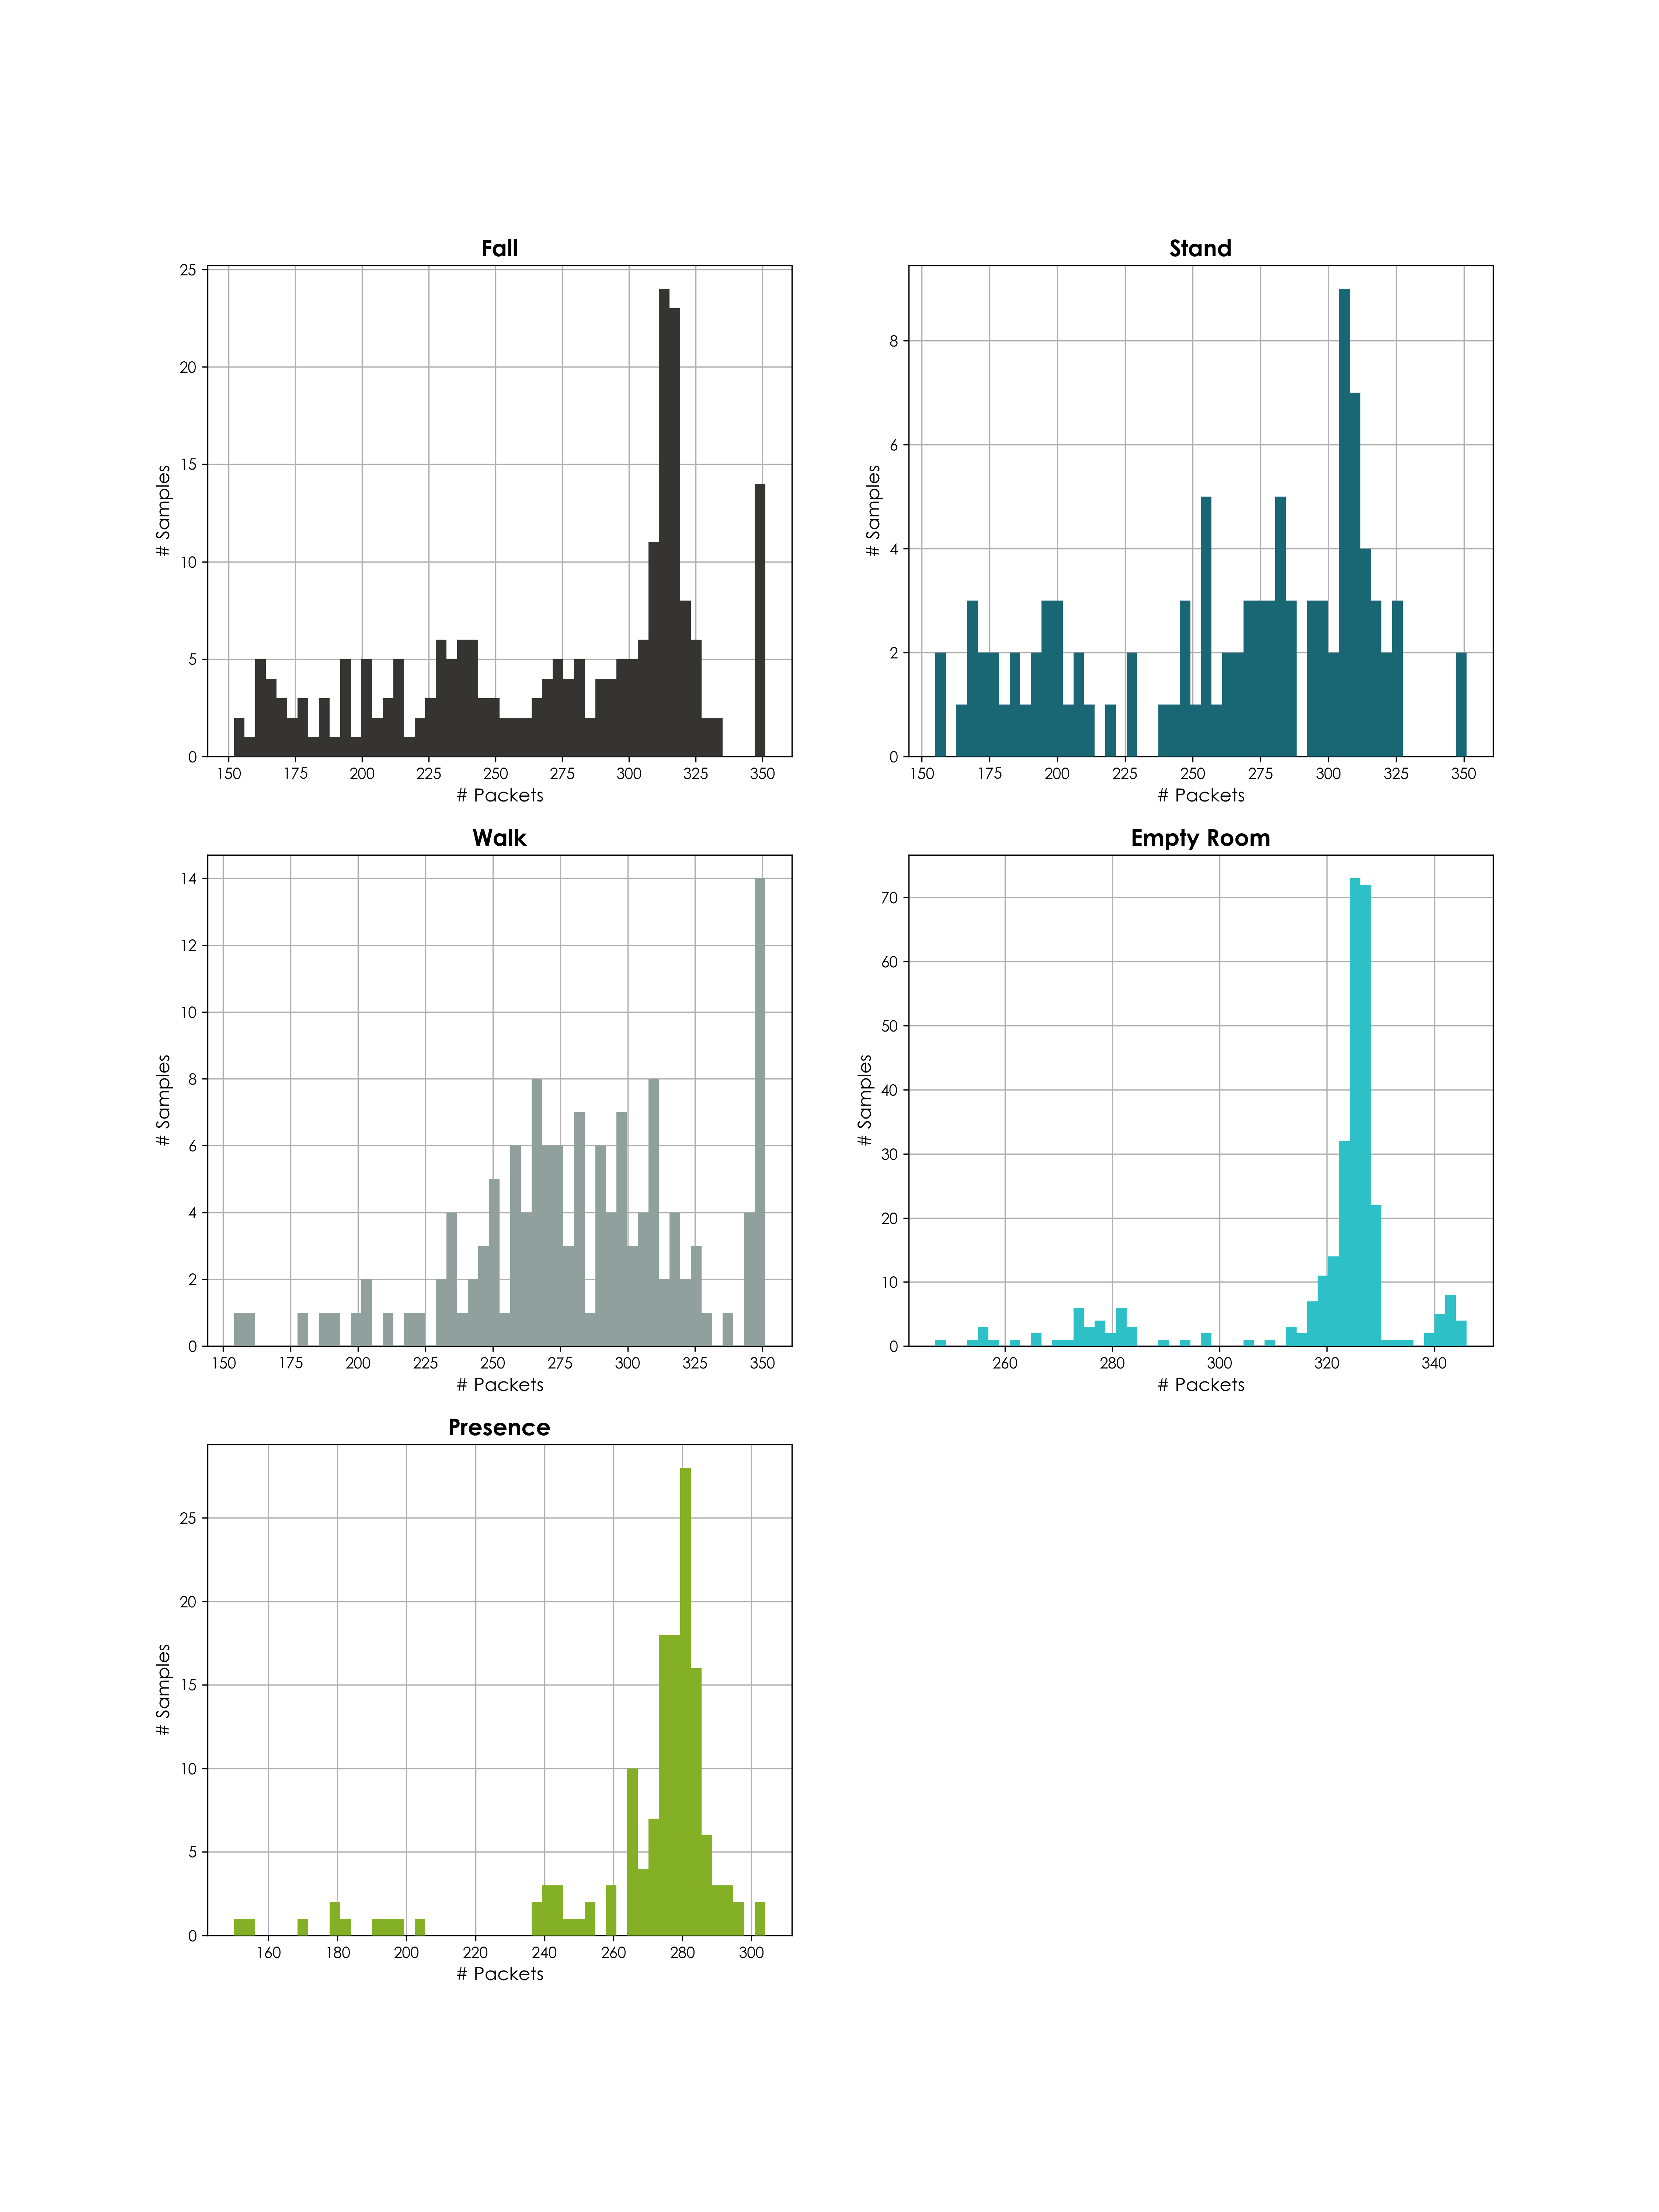
\includegraphics[width=1.0\textwidth, trim={0 6cm 0 4cm},clip]{./figure/chap 4/activity_data_sizes.png}
\caption{Packet counts of segments for different activities}
\label{Fig 4.9}
\end{figure}

\subsection{Subjects}
The number of subjects is an important aspect of any dataset. A higher number of subjects increase the generalized performance of any system. 13 subjects voluntarily performed different activities for this dataset. Most of the subjects have performed three different activities and some of them performed two or four activities out of five. In total, the subjects performed 20 to 45 segments of different activities.

\begin{figure}[H]
\centering
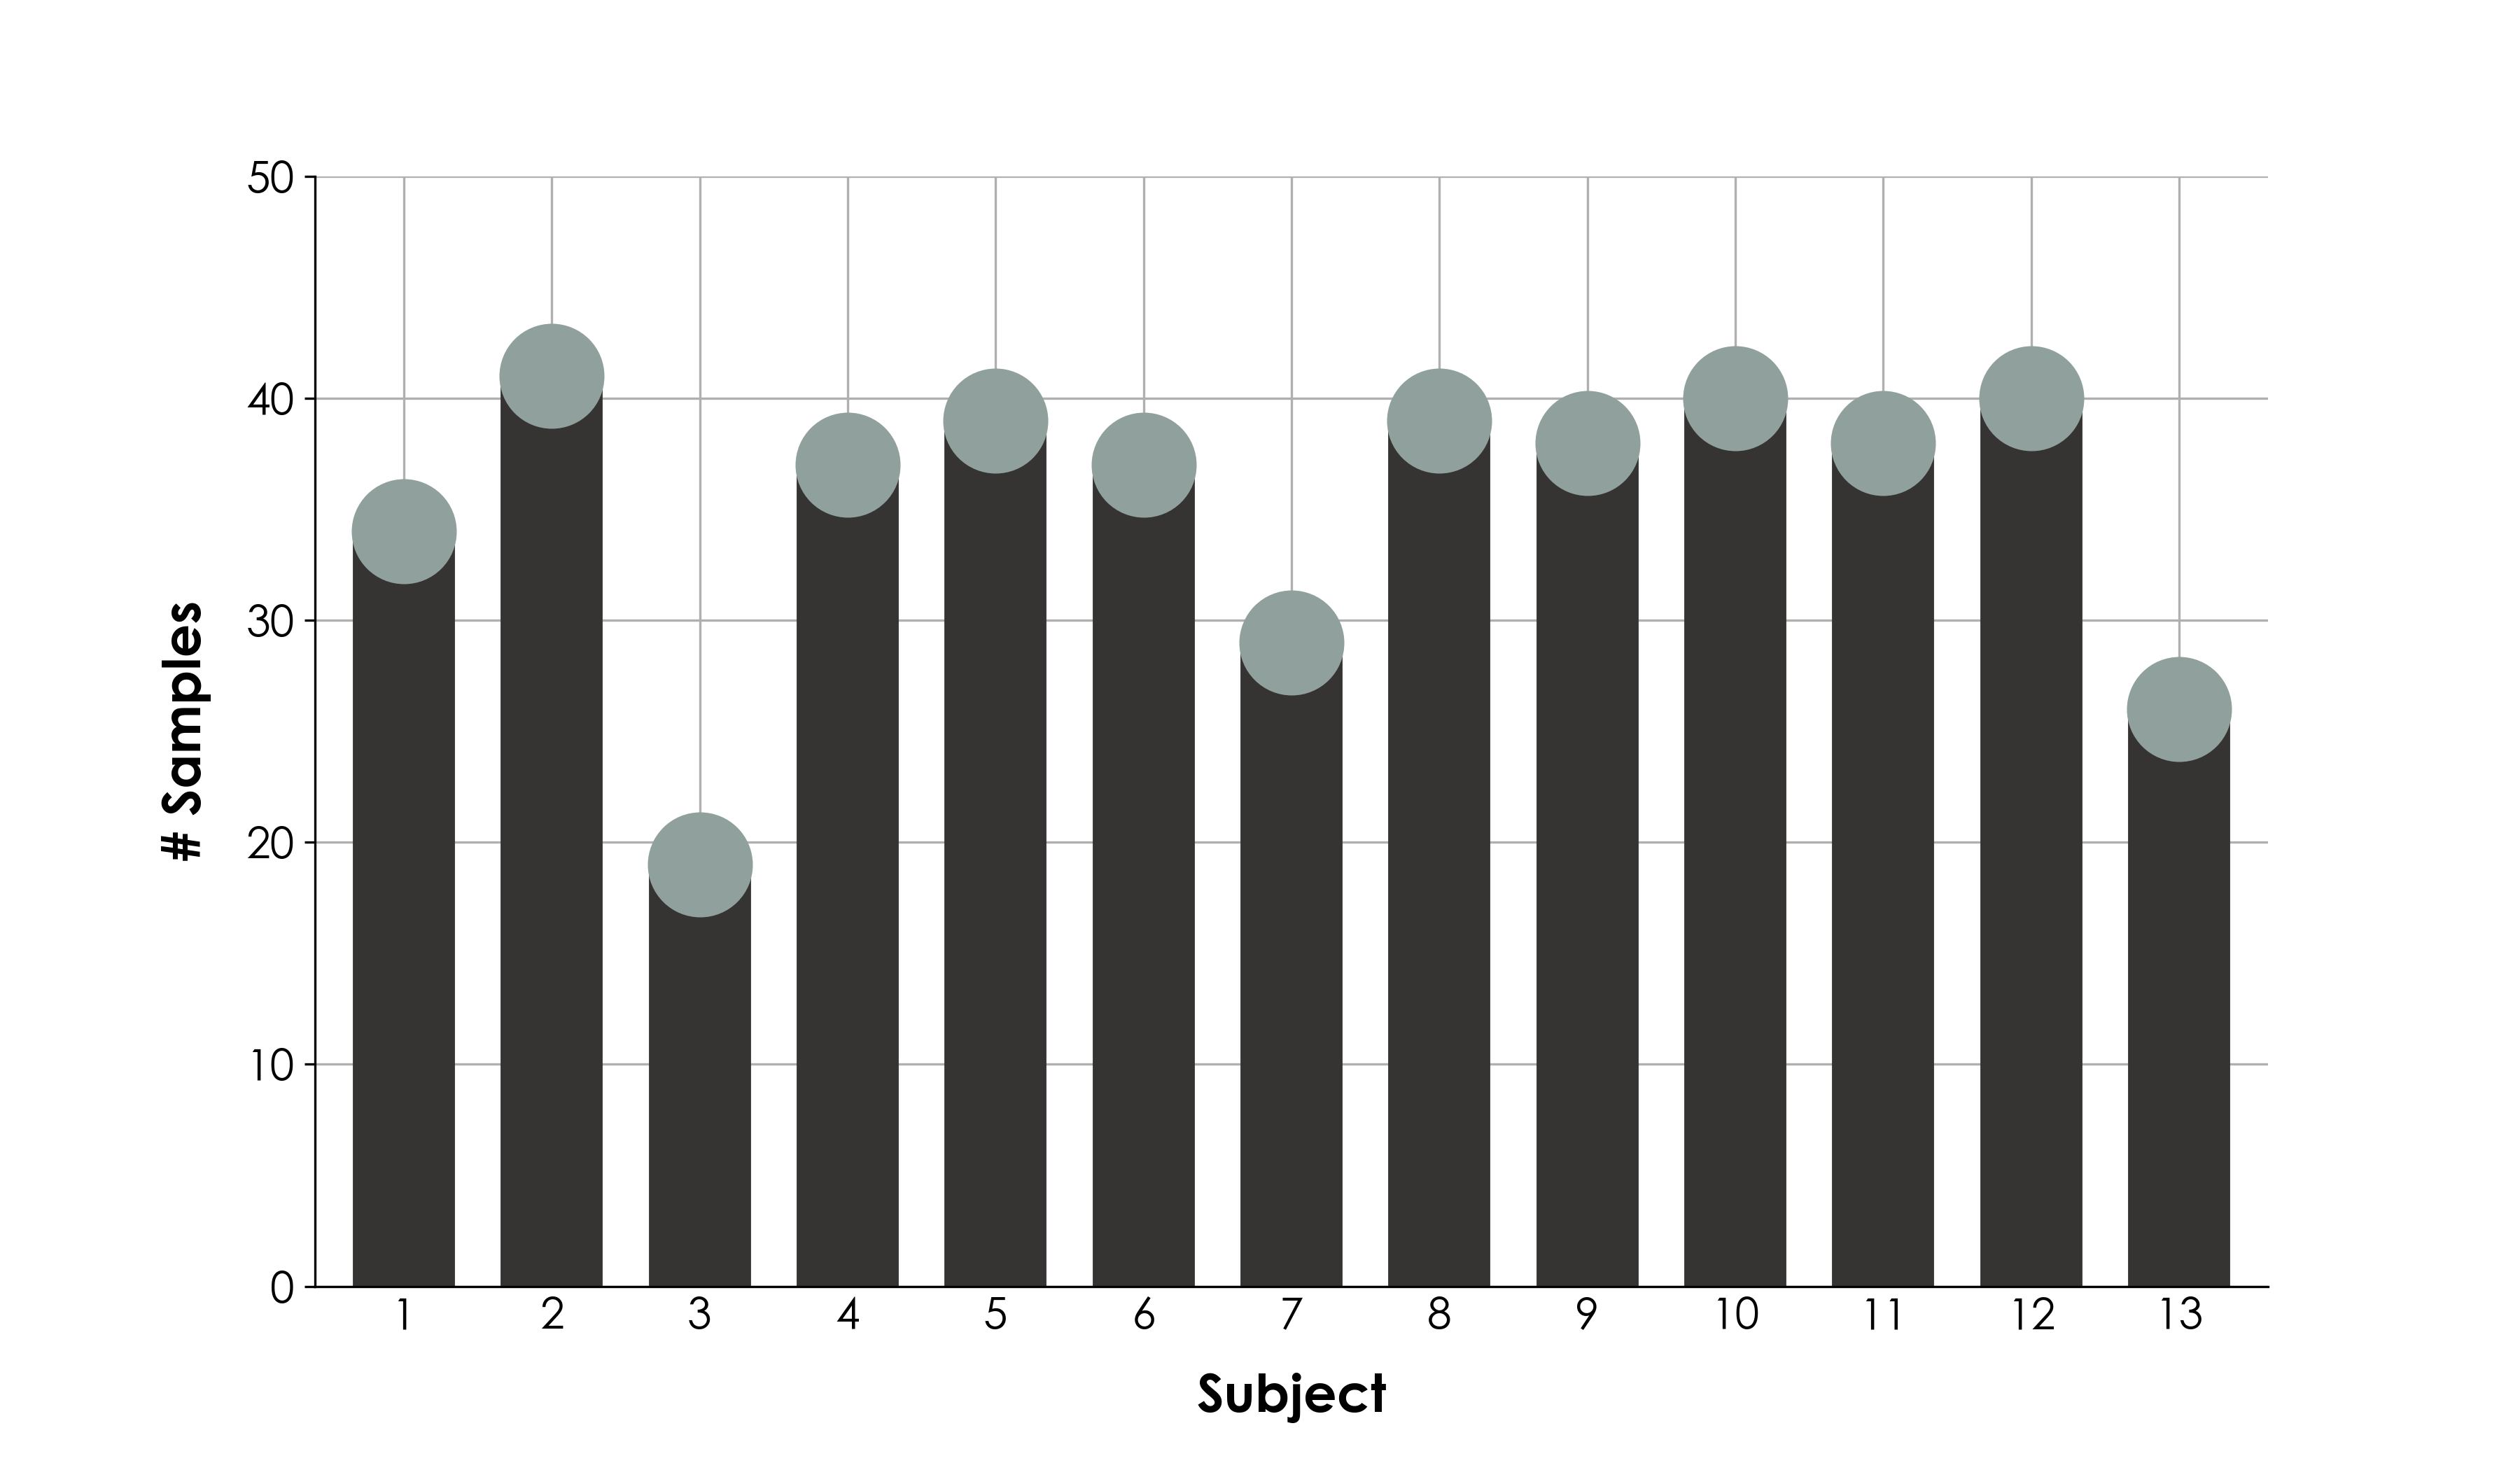
\includegraphics[width=1.0\textwidth]{./figure/chap 4/subjectwise_data_counts}
\caption{Number of samples by subject}
\label{Fig 4.10}
\end{figure}

\subsection{Dataset Summary}
Different aspects of the dataset is summarized in \ref{Table 4.3}.

\begin{table}[H]
\caption{Dataset summary}
\vspace{2mm}
\centering
\begin{tabular}{|l|c|} 
\hline
\multicolumn{1}{|c|}{\textbf{Specification}} & \multicolumn{1}{c|}{\textbf{Value}}                                                      \\ 
\hline
Device used             & ESP32-WROOM-32E             \\
Signals used            & CSI, RSSI                   \\
Activities              & 5                           \\
Subjects                & 13                          \\
Subject age range       & 18-25                       \\
Total samples           & 966                         \\
Selected samples        & 898                         \\
Sampling rate           & 100 Hz                      \\
Each sample time window & 4 seconds                   \\
Mean packet count       & 287                         \\
Room temperature        & 25 $^{\circ}$ C             \\
\hline
\end{tabular}
\label{Table 4.3}
\end{table}


\section{Data Preprocessing Pipeline}
The data we collected includes the raw signal information and packets. In this section, we propose a robust and complex preprocessing pipeline to preprocess the raw data and make the raw data used for the system. At first, we need to extract the CSI data from the raw signal and isolate the phase and amplitude information from it. As CSI data is inherently sensitive to different environmental parameters, some cleaning process needs to be applied such as calibration, denoising, and dimensionality reduction. There are various denoising algorithms to choose from. We compare their performances and choose the best one. After preconditioning the signals, we feed the data to the feature extraction module that extracts different features from the cleaned data. Not all the features are important for the outcome. So, we have to use different mathematical models to find the most relevant features. A normalization technique is employed before handing the data over to a competent machine learning model. Lastly, we tune different hyperparameters of the model to increase the performance of the model on the dataset. 

\begin{figure}[H]
\centering
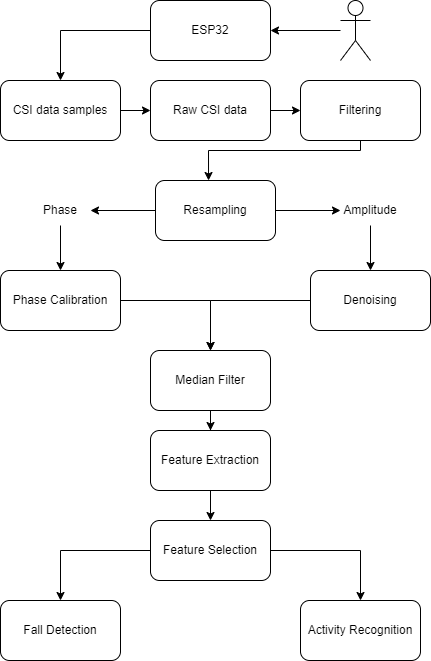
\includegraphics[width=0.7\textwidth]{./figure/chap 4/csiProject.drawio.png}
\caption{Complete Pipeline of The System}
\label{Fig 4.11}
\end{figure}

\subsection{CSI Data Extraction}
CSI essentially enables us to comprehend what transpires on the channel between the transmitter and receiver. CSI is calculated by examining how the preamble with known content is changed during transmission. Thus, we have a collection of complex numbers in the form $a_{n} \exp j \theta_{n}$, where $a_{n}$ is the amplitude and $ \theta_{n}$ is the phase. We need to extract this amplitude and phase from the raw CSI data. A raw CSI packet comprises the real and imaginary part of the channel state and is transmitted separately for each subcarrier. But not all subcarriers carry useful information. Different subcarriers respond differently to human activity; for example, certain subcarriers are quite sensitive to motion and exhibit obvious fluctuations. It is preferable to use only the CSI information from these sensitive subcarriers. The computing complexity of the system is also increased by using all of the data from all of the subcarriers. So, we removed some of the irrelevant subcarriers by examining the acquired CSI sequence, and skillfully isolate the signal segments mostly corresponding to human activity. Then we transformed the real and imaginary parts of the selected subcarriers into polar form to get the required amplitude and phase information.

\subsection{Time Series Representation}
The extracted CSI data ideally should be a time series having a constant time difference between two samples. But in practice, the sampling rate was not constant and there was a considerable amount of packet loss which led to non-uniform data. To apply different time and frequency domain analysis, this data need to convert to a time series representation. That's why we resampled the data at a constant 100 Hz sampling rate. This process involves resulting in some missing values which are linearly interpolated to generate an equivalent waveform.

\begin{figure}[H]
\centering
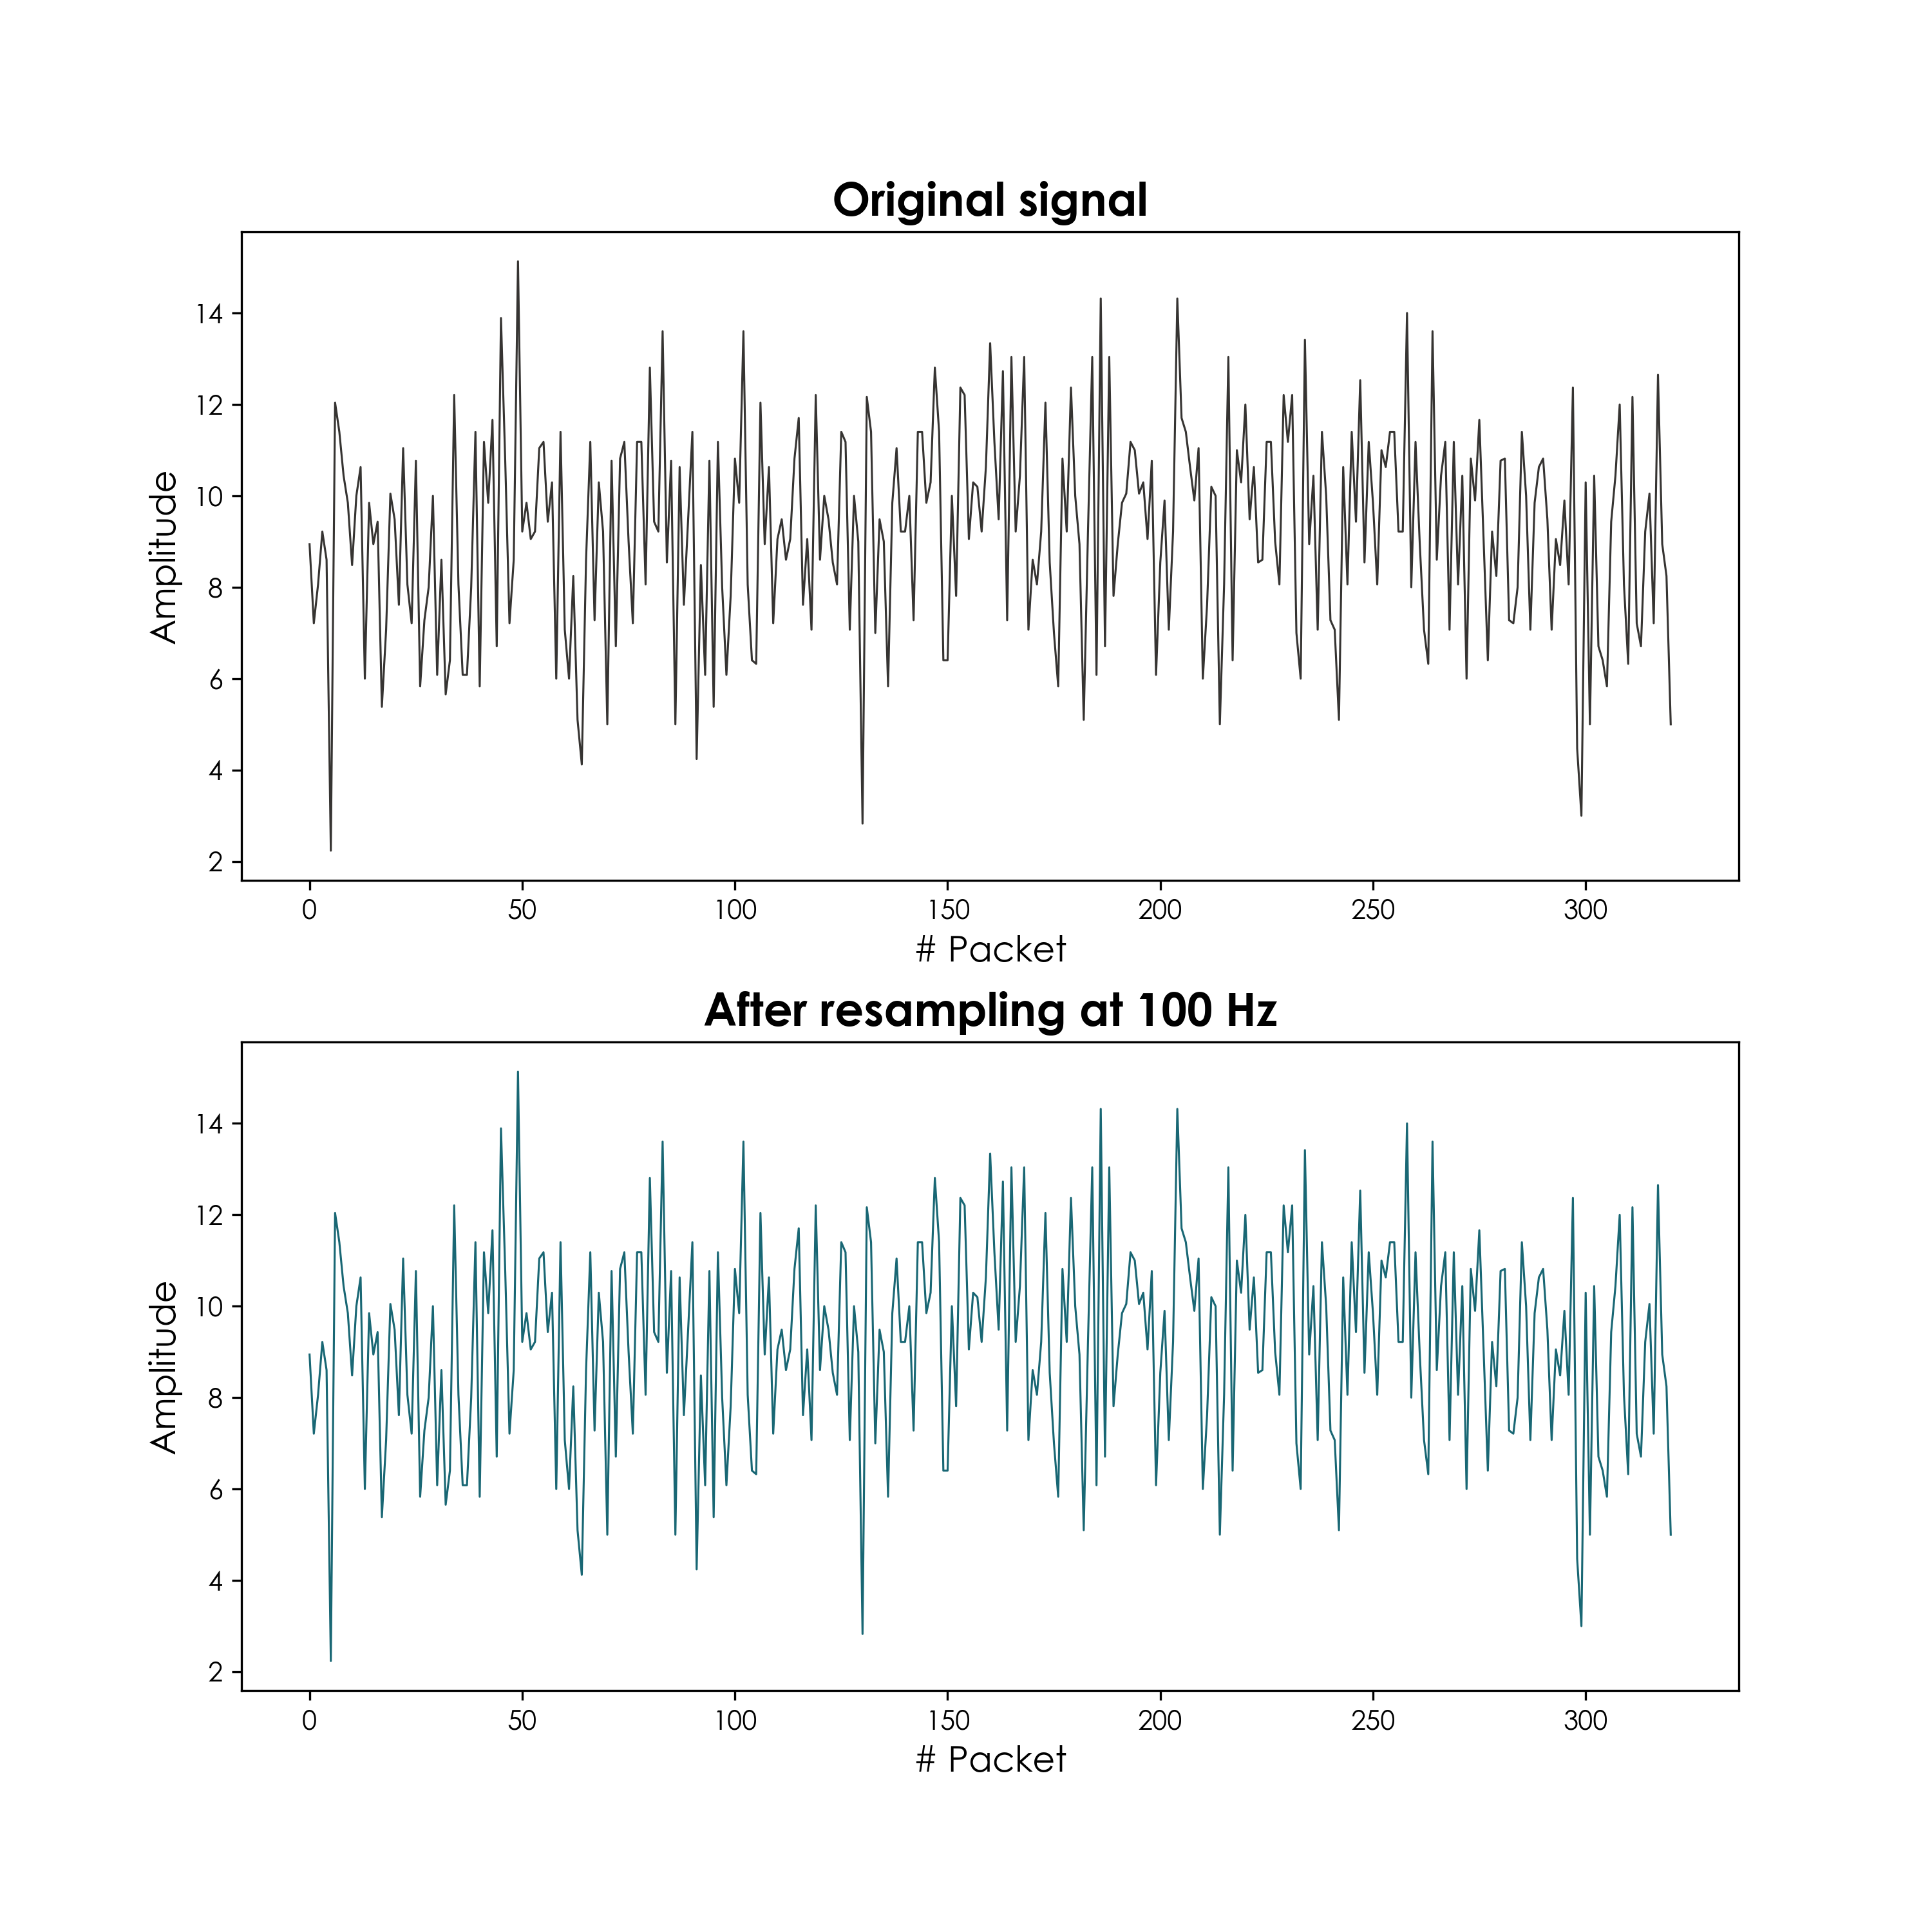
\includegraphics[width=1.0\textwidth, trim={0 1cm 0 0} , clip]{./figure/chap 4/resampling_plot.png}
\caption{Resampling for time series representation}
\label{Fig 4.12}
\end{figure}


\subsection{Phase Signal Analysis}
The isolated phase information of $i^{th}$ subcarrier can be expressed by the following equation:
\begin{equation}
    \hat{\phi _i} = \phi _i - 2\pi \frac{s_i}{N}\tau + \beta + Z
\end{equation}
Here, $\phi_i$ is the actual phase which is deteriorating by the time offset at receiver $\tau$, unknown time offset $\beta$, and measurement error $Z$. $s_i$ is the subcarrier index and $N$ signifies the Fast Fourier Transform (FFT) size which is 64 for IEEE 802.11n. Due to this distortion, the phase must be calibrated the restore the actual phase as much as possible. As shown by \cite{10.1145/2307636.2307654}, the time offsets, $\tau$, and $\beta$ can be removed by considering the phase across the frequency band given by the equation:
\begin{equation}
    \hat{\phi _i} =  \hat{\phi _i} - as_i - b =  \hat{\phi _i} - \frac{\phi _n - \phi _1}{s_n - s_1} s_i - \frac{1}{n} \sum_{j=1}^{n} \phi _j
\end{equation}
Here, $a$ and $b$ are intermediate variables. 
But in this process, the true phase is folded due to
the recurrence characteristic of the phase. This problem can be solved by compensating multiple $2\pi$’s by judging whether the measured phase change between the adjacent subcarriers is greater than the given thresholds \cite{7460092}.

\subsection{Denoising Amplitude Signal}
The amplitude of the CSI data is very sensitive to internal and external noises. Possible noise sources are scattering, reflection, delay, fading, and power line losses. The signal can be denoised by using various techniques including different filters or transformations.

\begin{figure}[H]
\centering
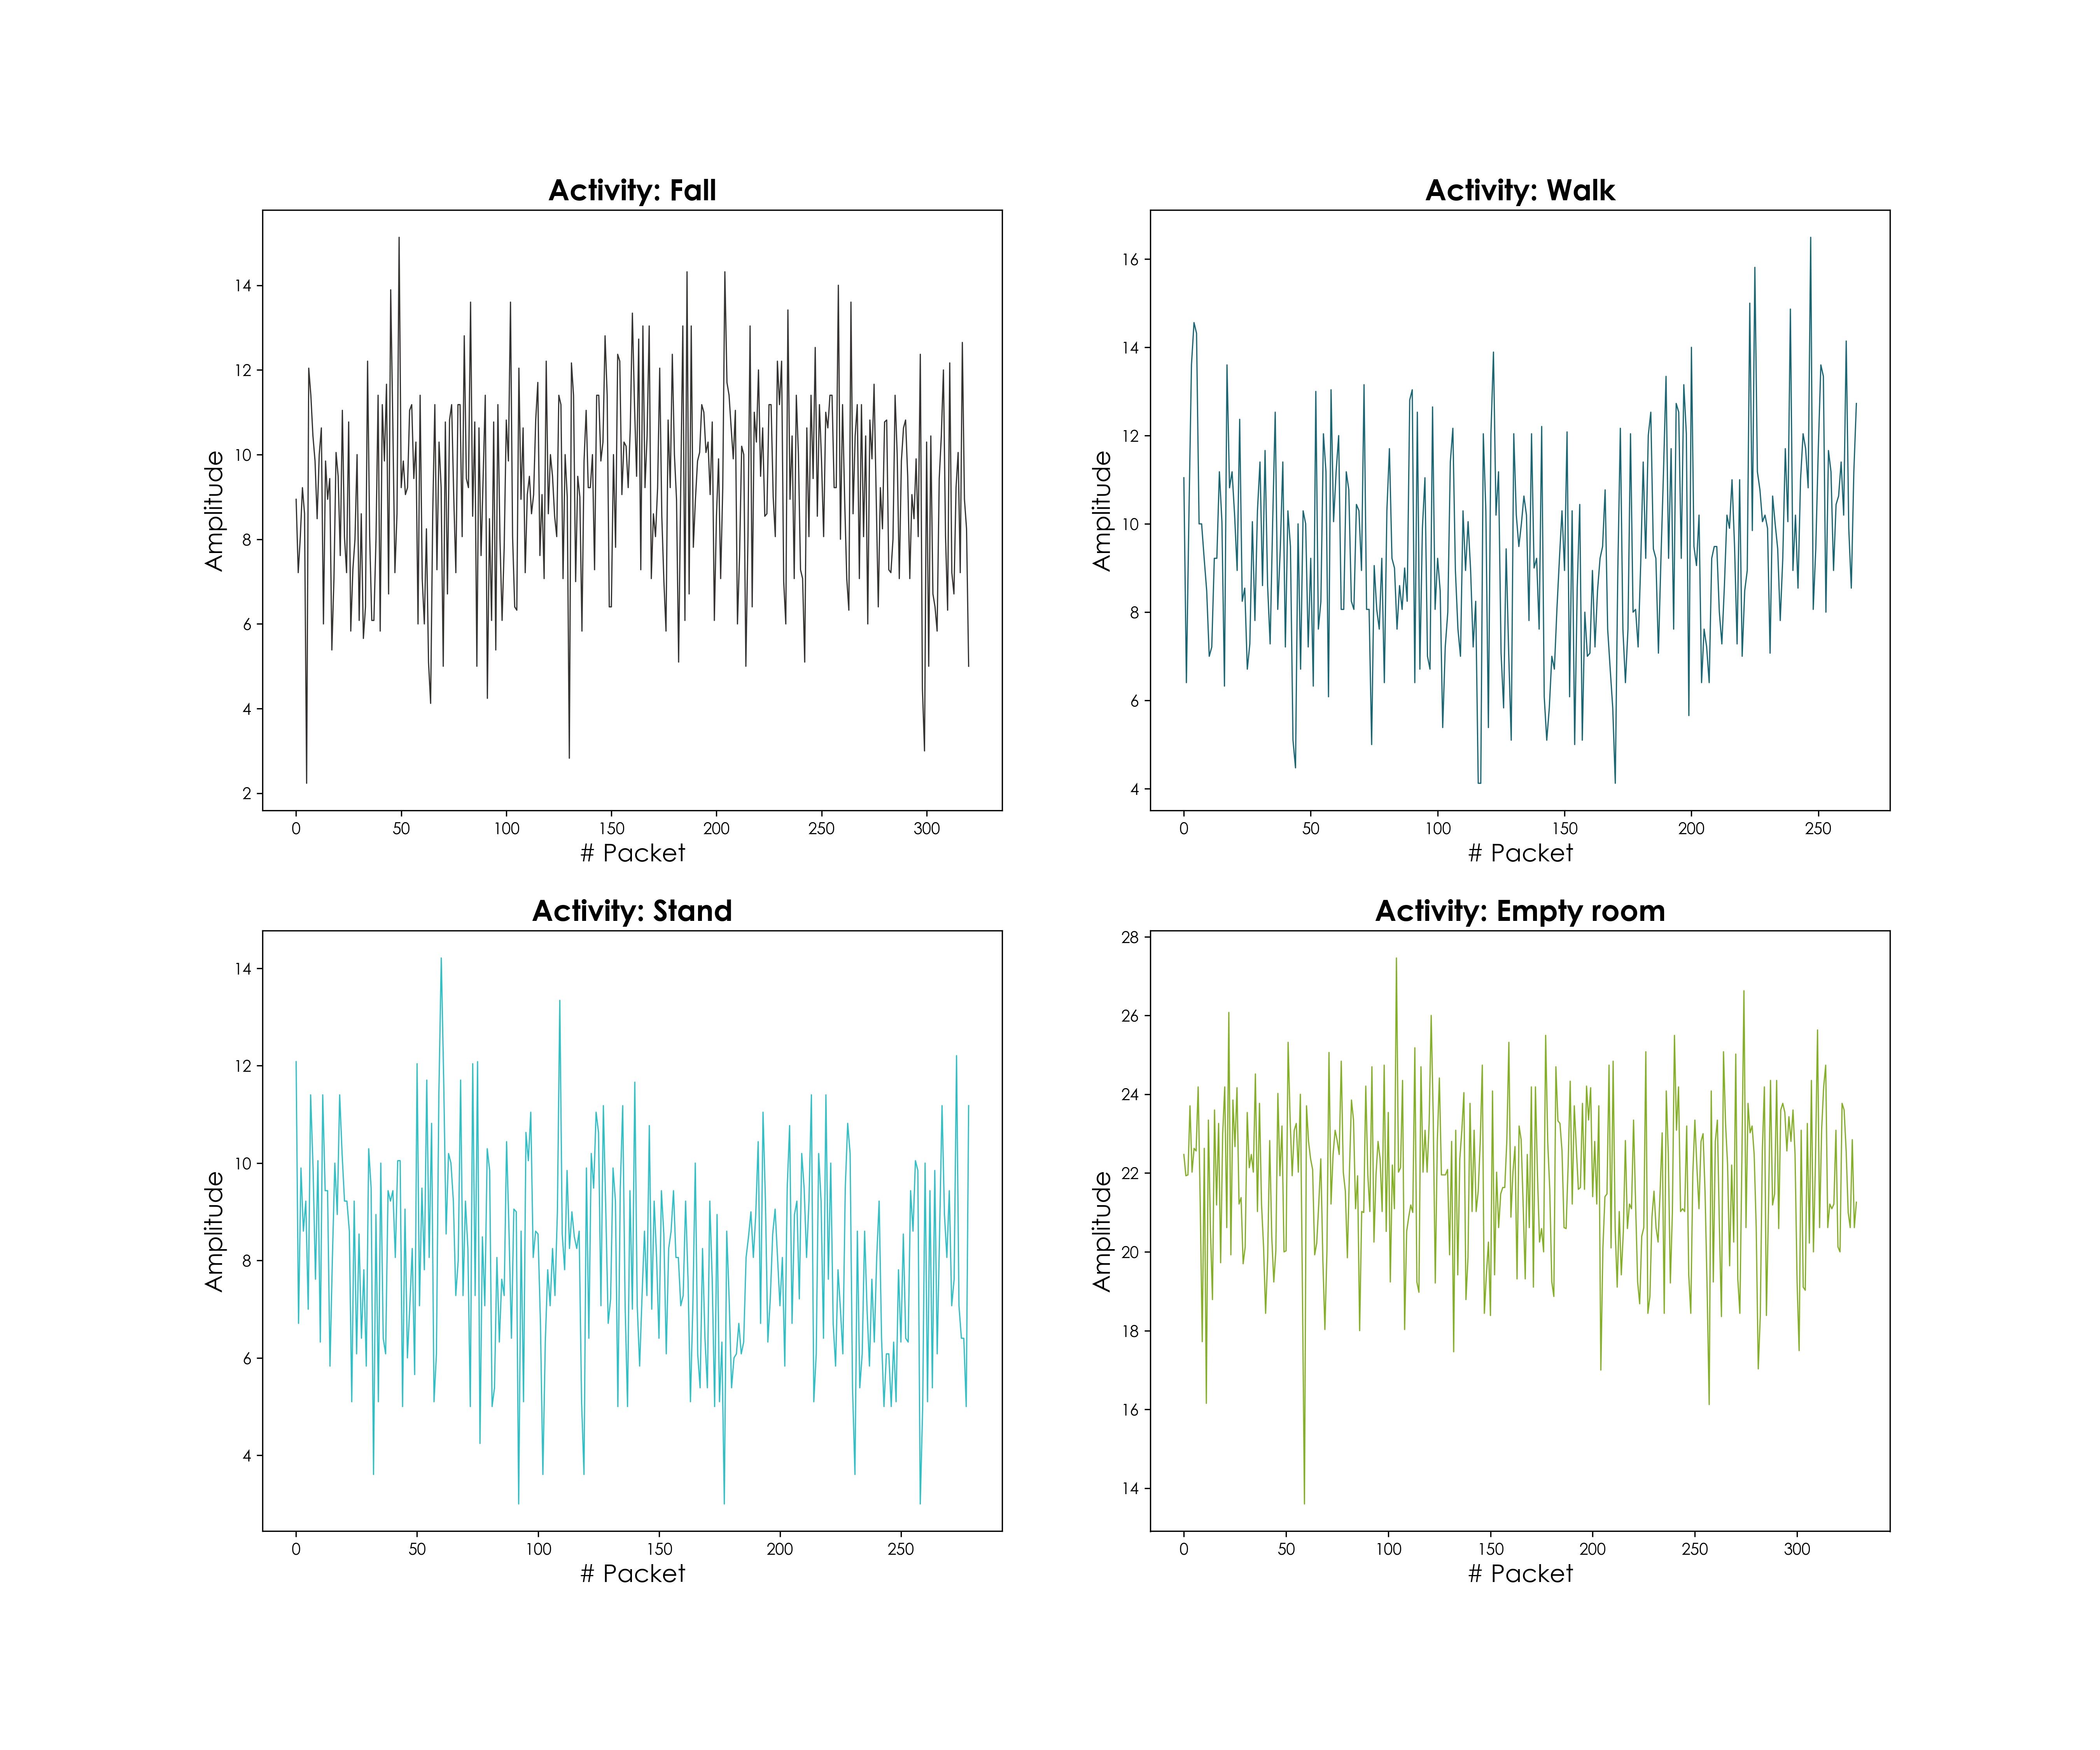
\includegraphics[width=1.0\textwidth, trim={0 3cm 0 2cm},clip]{./figure/chap 4/magnitude_plot_raw.png}
\caption{Raw CSI amplitude signal for different activities}
\label{Fig 4.13}
\end{figure}

\subsubsection{Low Pass Filter (LPF)}
A low-pass filter is a filter that attenuates the higher frequency portion of a signal than a chosen cutoff frequency. The filter's precise frequency response is determined by the filter's design. There are many types of low pass filters, but in this project, we will focus on a specific type named \emph{Butterworth filter} \cite{butterworth1930theory}. Butterworth filter is a signal processing filter made to have a frequency response that is as flat as possible in the passband.  Butterworth filter has a slower roll-off and thus will require a higher order to implement a particular stopband specification, but it has a more linear phase response in the passband than most others. Low pass butterworth filters are greatly used for noise removal from various signals. Generally, a noisy wave contains two different portions: high-frequency noise and low-frequency true signal. This also fits for CSI amplitude signal. Thus the high-frequency noise mixed in the signal can be removed by using a Butterworth low pass filter. But a problem with this method arises when the signal and noise frequency are not separated by a large margin. As butterworth filter has a slower roll-off, it tends to attenuate some of the original signals too. 

\subsubsection{Fast Fourier Transform (FFT)}
A fast Fourier transform (FFT) algorithm calculates a sequence's discrete Fourier transform (DFT) or its inverse (IDFT). Through the process of Fourier analysis, a signal is transformed from its original domain, which is frequently time or space, to a representation in the frequency domain, and vice versa. The DFT is produced by breaking down a series of numbers into components of various frequencies. [1] Although computing it straight from the specification is generally too time-consuming to be helpful, this technique has many applications. Such changes are quickly computed by an FFT by factorizing the DFT matrix into a product of sparse (mostly zero) elements.\cite{fft} This successfully reduces the complexity from    $O(N^2)$ to  $O(Nlog(N))$ where N is the number of samples.

\subsubsection{Short-Time Fourier Transform (STFP)}
A Fourier-related transform known as the Short-time Fourier transform (STFT) is used to ascertain the sinusoidal frequency and phase content of local parts of a signal as they change over time. To compute STFTs, it is necessary to split a longer temporal signal into equal-length shorter segments. Each shorter segment is then subjected to a separate Fourier transform computation. This makes each shorter segment's Fourier spectrum visible. The shifting spectra are then typically plotted as a function of time using a technique called a spectrogram or waterfall plot, which is frequently applied in Software Defined Radio (SDR)-based spectrum displays. On desktop PCs, Fast Fourier Transforms (FFTs) with $2^{24}$ points are frequently used for full bandwidth displays that span the whole SDR range.\cite{stft}

\subsubsection{Wavelet Transform (WT)}
In Fourier transform (FT), we represent a function using a series of sine and cosine waves, which is an excellent approach to understanding the frequencies present in the signal. However, it has a significant drawback. FT only contains the frequency information, but the spatial or temporal information is completely lost. It will not be possible to tell where the frequency is low or high in the space or time domain, or where frequency shifts are taking place. To overcome this problem, we do Wavelet Transform (WT). In WT, we represent a function using a certain orthonormal series produced by a wavelet. A wavelet is a waveform of effectively limited duration that has an average value of zero and nonzero norm. If a function $\phi$ can provide a Hilbert basis or a full orthonormal system, for the Hilbert space of square-integrable functions, then $\phi$ is referred to as an orthonormal wavelet. The fundamental principle of wavelet transform is that they should only be able to modify the length of time, not shape. This is impacted by selecting appropriate base functions that support this. Changes to the time extension should match up with the analysis frequency of the basis function. 

\subsubsection{Discrete Wavelet Transform (DWT)}
A discrete wavelet transform (DWT) \cite{shensa1992discrete} decomposes an input signal into several sets, each set consisting of a time series of coefficients that describe the signal's temporal evolution in the associated frequency band. In this process, the wavelets are sampled in discrete steps. A key advantage it has over Fourier transforms is temporal resolution: it can show both frequency and location information (location in time). The DWT refers not just to a single transform, but rather to a set of transforms, each with a different set of wavelet basis functions. Two of the most common are the Haar wavelets and the Daubechies set of wavelets. Unlike the Continuous Wavelet Transform (CWT), it uses a finite set of wavelets, i.e., defined at a particular set of scales and locations. But the main idea remains the same; we multiply the signal with a particular wavelet with a particular scaling and then shift it over the whole signal to integrate. In DWT, we repeat the procedure after changing the scale. In these situations, scaling adjustments are made discretely.
The DWT can be defined by the following equation:
\begin{equation}
    T_{m,n} = \int_{-\infty}^{\infty} x(t) \psi _{m,n} (t) dt 
\end{equation}

where $\psi$ is the wavelet function. The components of the signal can be assembled back into the original signal without loss of information using a reconstruction algorithm known as the Inverse Discrete Wavelet Transform (IDWT). In IDWT, the DWT coefficients are first upsampled by inserting zeros between each coefficient, essentially doubling the length of each (the approximation and the detail coefficients are handled separately). The reconstruction scaling filter for approximation coefficients and the reconstruction wavelet filter for detail coefficients are then convolved with these. To get the original signal, these results are then put together. 

\subsubsection{Comparison of DWT and LPF}
For our dataset, we employed two different types of denoising methods. One is a $4^{th}$ order Butterworth low pass filter with a cut-off frequency of 10 Hz. The other is a second-level Discrete Wavelet Transform using symlet10 wavelet. 

\begin{figure}[H]
\centering
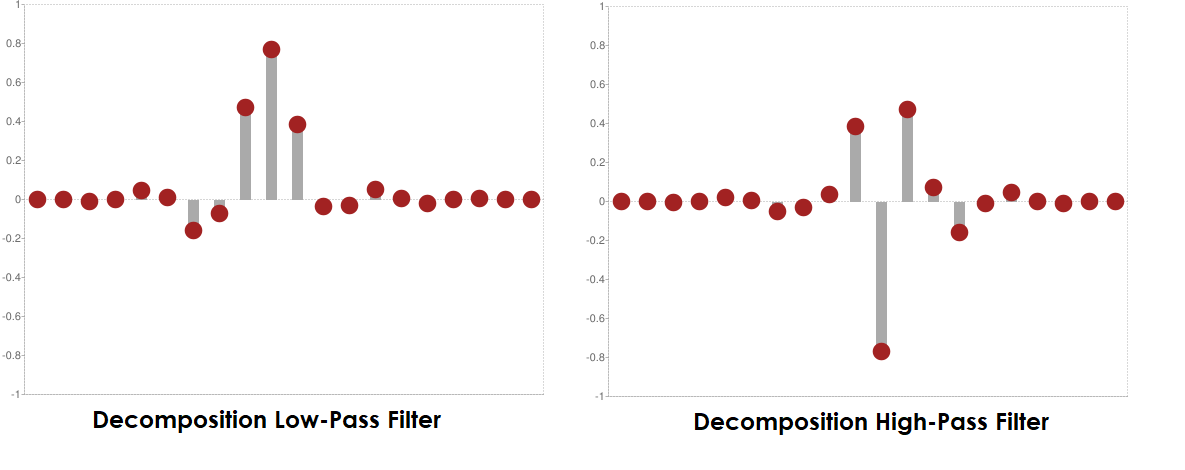
\includegraphics[width=1.0\textwidth]{./figure/chap 4/sym10.png}
\caption{Symlet10 wavelet}
\label{Fig 4.14}
\end{figure}

We used both denoisers and compared how they work on different CSI amplitude waves. By careful comparison, we found the DWT denoising method performed better than low pass filter. So, we chose DWT denoising for this system.

\begin{figure}[H]
\centering
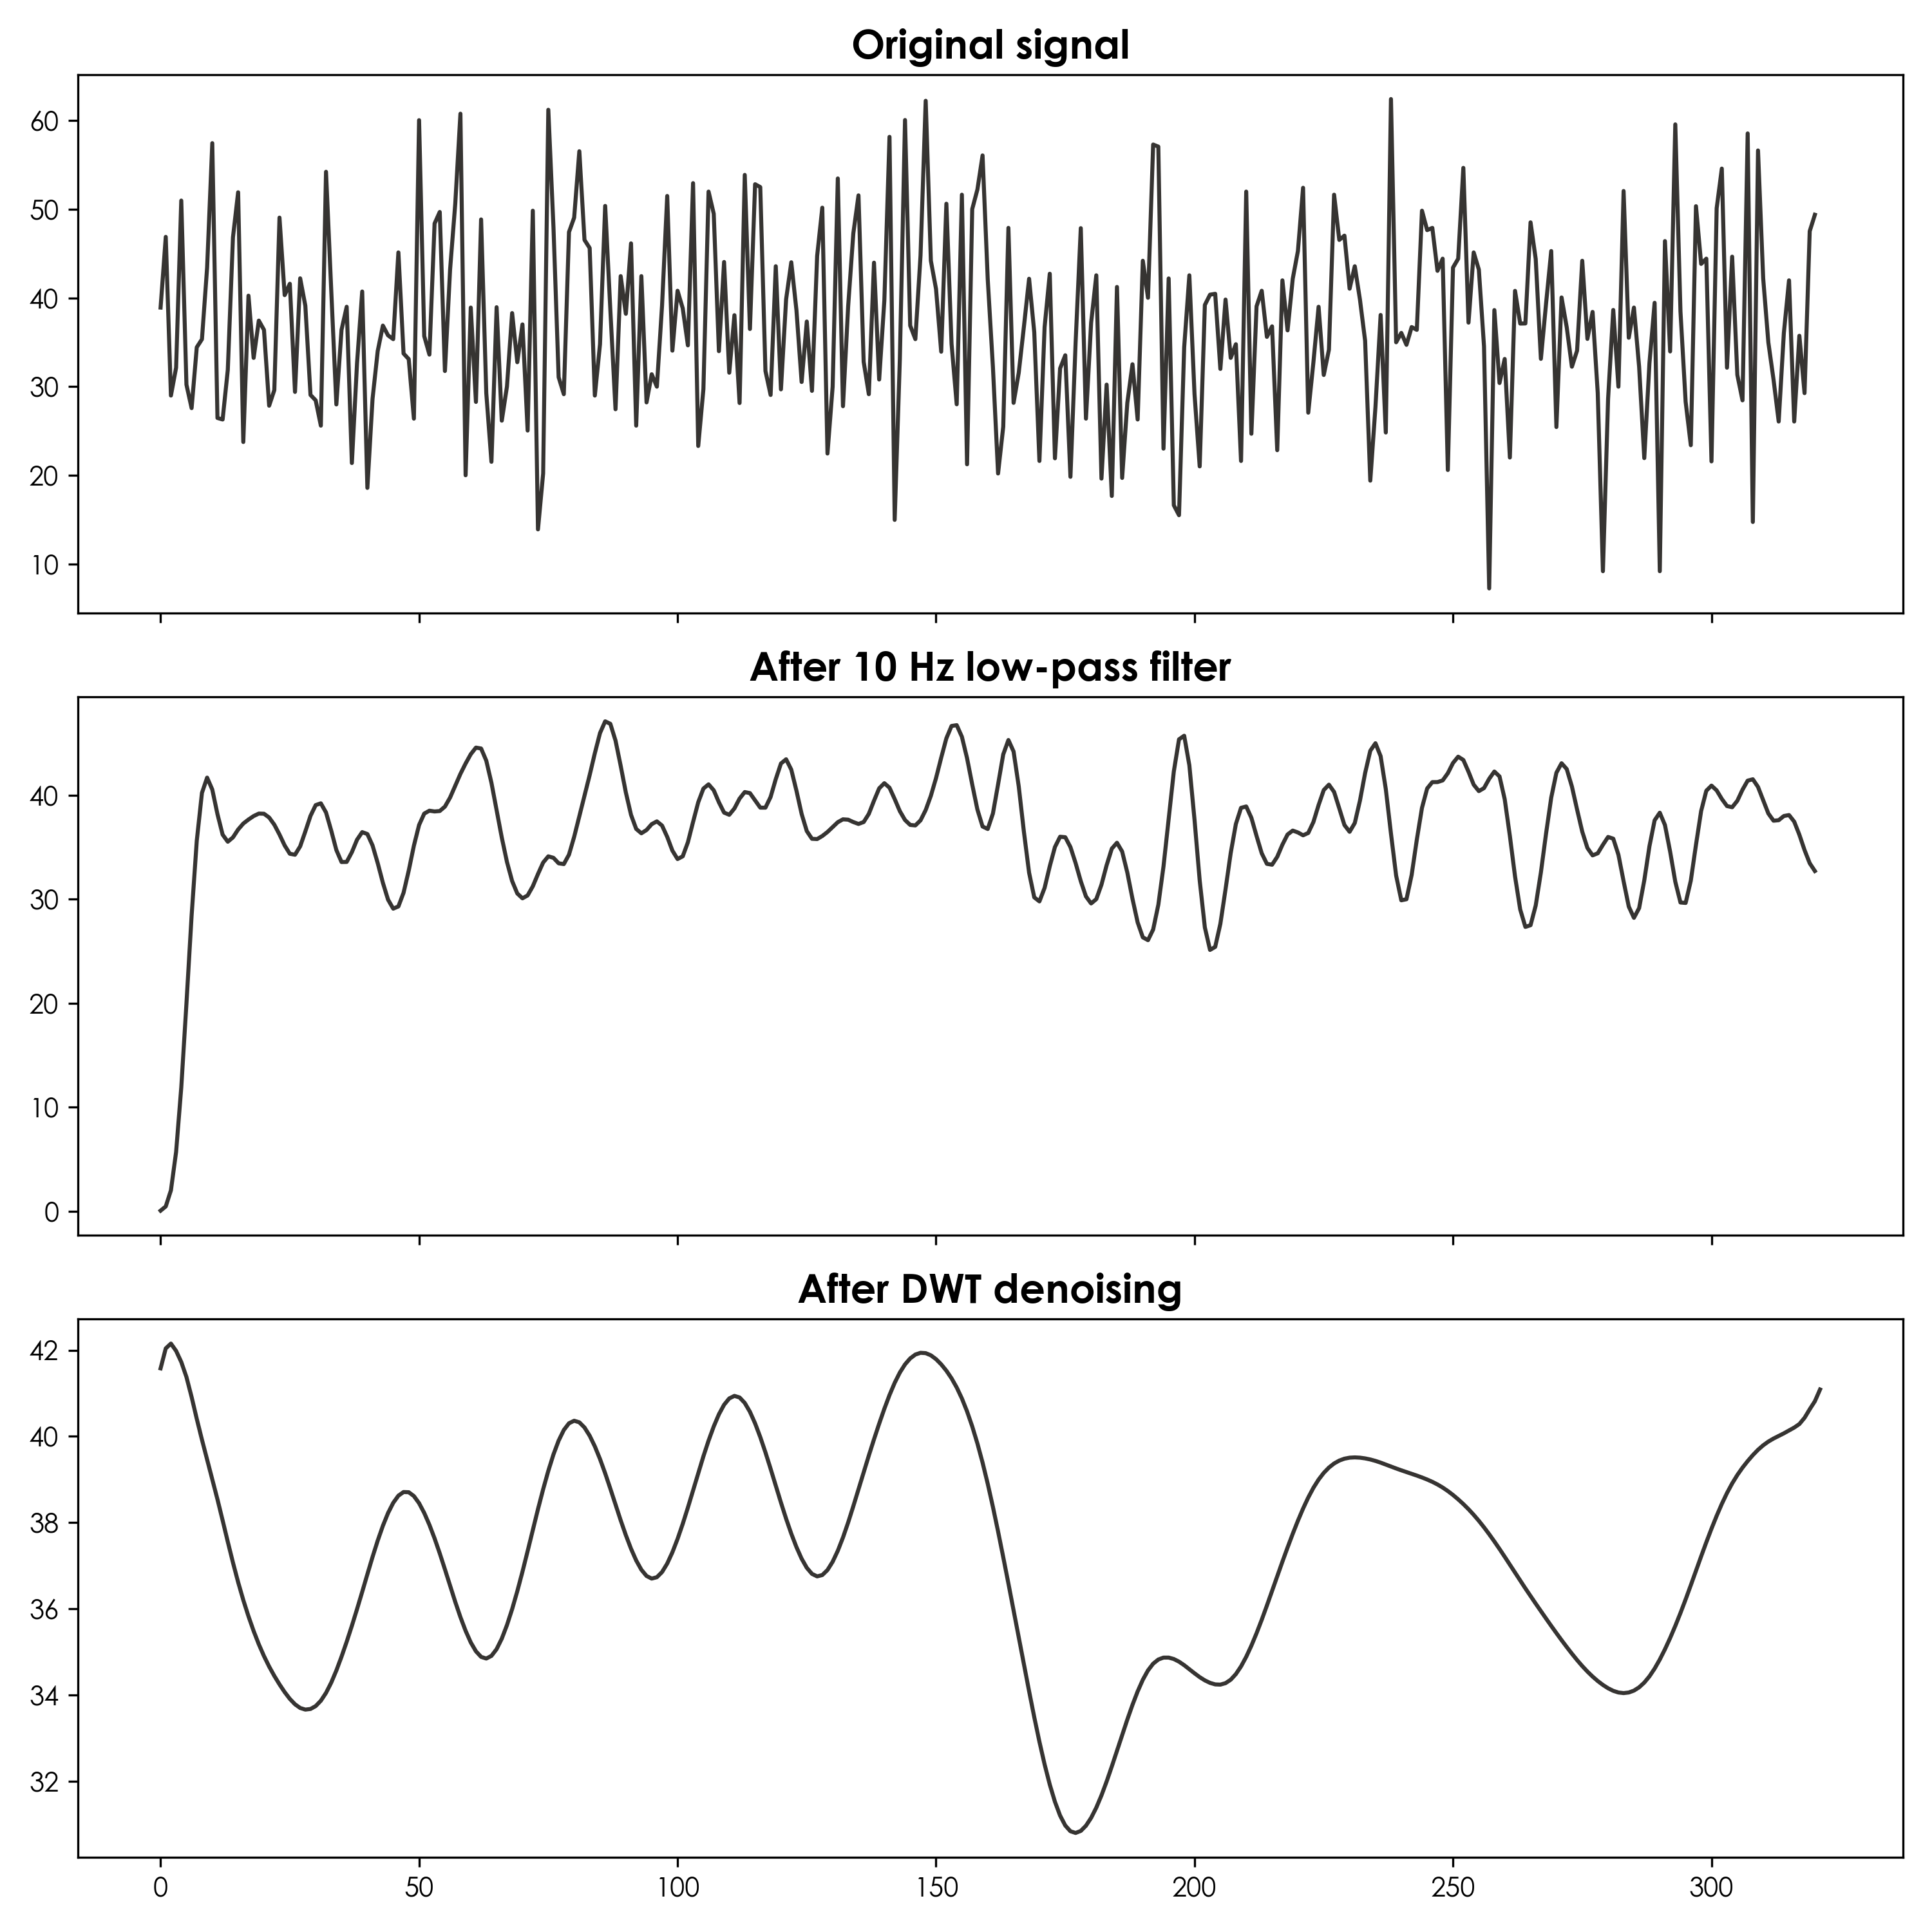
\includegraphics[width=1.0\textwidth]{./figure/chap 4/lpf_vsdwt.png}
\caption{Comparison between low pass filter and DWT}
\label{Fig 4.15}
\end{figure}

\section{Feature Selection}
After conditioning and denoising the signals, we extracted some statistical features including min, max, median, and standard deviation from the phase and amplitude CSI and RSSI signals. But the initial feature size was 716 which is very large considering the sample size which is only 898. So, we needed to prune the feature set to remove non-correlated features. There are different ways to measure the correlation or importance of the features with the output variable.

\subsection{Chi-Square Test \cite{chisquare}} 
One technique to demonstrate a connection between two categorical variables is via a chi-square statistic. The chi-squared statistic is a single figure that indicates the degree to which the counts you saw deviate from the counts you would anticipate if there were no association at all in the population. 

\begin{equation}
    \chi_c^2 = \sum \frac{(O_i - E_i)^2}{E_i}
\end{equation}

\subsection{Pearson's Correlation Coefficient (PCC) \cite{pcc2020}}
Pearson’s correlation coefficient is the test statistics that assess the statistical association, or relationship, between two continuous variables. Because it is based on the method of covariance, it is regarded as the best method for determining the relationship between variables of interest. It provides details on the size of the association or correlation as well as the relationship direction. One problem with PCC is that it is not able to tell the difference between dependent variables and independent variables.

\subsection{Decision Tree (DT) based feature selection \cite{dtfeatureselection}}
Decision tree building algorithm selects the splits locally, i.e. concerning the splits selected in earlier stages, so that the features occurring in the decision tree, are complementary. Thus, Decision Tree based models provide feature importance metrics that can be utilized to select the most important features. 

We used a combination of PCC and decision tree-based selection methods to select the most important 243 features for our proposed method.


\section{Training Description}
Every supervised machine learning system has three phases: 
\begin{enumerate}
    \item Training phase: We train the data for the known labels.
    \item Testing phase: We evaluate the performance of the trained model keeping the labels away from the model.
    \item Application phase: We apply our model for real-life unknown data.
\end{enumerate}

Our proposed preprocessing pipeline is independent of the training phase. So, it gives us the advantage to use any machine learning model for our preprocessed data even for different learning tasks. In this project, we have two different learning objectives. One is \emph{fall detection} and the other one is a generalized \emph{human activity recognition}. 
\subsection{Fall Detection}
For fall detection, we classified the \emph{walk} and \emph{stand} activities as non-fall activity, kept the \emph{fall} activity as is and did not use the \emph{empty room} and \emph{presence} activities. Then, we trained binary classification algorithms on this data.
\subsection{Human Activity Recognition}
In this objective, we utilized the whole dataset with all the activities, i.e., \emph{fall}, \emph{stand}, \emph{walk}, \emph{empty room} and \emph{presence}. So, we have five labels in this task and used this data in different multi-class classification algorithms.

In both cases, we compared the behavior and performance of these algorithms and tuned them to get the best performance on the test set. The performance statistics of these models are depicted in the next chapter.



\chapter{RESULT AND ANALYSIS}
 \label{Chapter 5}
 \lhead{Chapter 5. \emph{Result \& Analysis}}
 

In this chapter, we aim to discuss the results of our implementation and analyze its performance in various scenarios and test setups.

\section{Evaluation Metrics}

\textbf{Classification Accuracy:}
Classification Accuracy is what we usually mean by the term accuracy. It is the highest used metric for classification tasks which works best when the number of samples belonging to each class is nearly equal. But, it does not convey any useful information when the dataset is imbalanced. For example, if any dataset has two classes: class A, and B, and 98\% of the dataset belongs to class A, blindly predicting each of the samples as class A will give an accuracy of 98\% which is misleading. Hence, this metric is only used in balanced datasets.
\begin{equation}
    Accuracy = \frac{\#\:correct\:predictions}{\#\:all\:samples}
\end{equation}

\textbf{Precision:}

precision is a measure of result relevancy, it calculates how many positive predictions are correct. It focuses on the correctness of positive detection which can be a good metric for cases where a false positive can be more troublesome than a false negative. 

\[ Precision = \frac{TP}{FP + TP}\]

\textbf{Recall:}
Unlike precision, Recall focuses on correctly identifying True Positives out of all the positive samples. It can be referred to it as Sensitivity or True Positive Rate.  It is a good metric where false negatives are more troublesome, such as in disease detection.

\[ Recall = \frac{TP}{FP + FN}\]

\textbf{F1 Score:}
It is a metric combination of both the Precision and Recall scores. It lets us do a tradeoff between Precision and Recall. A good F1 score is the indication of both good Recall and good Precision. That is why F1 score is considered one of the most important metrics to evaluate the performance of a classification system.

\[ F1\:Score = 2*\frac{Precision*Recall}{Precision + Recall}\]

\textbf{Area Under Curve (AUC):}
It is also known as AUC-ROC which signifies the area under the Receiver Operating Characteristic (ROC) curve. The ROC curve is an evaluation metric initially proposed for binary classification problems. In essence, it separates the "signal" from the "noise" by plotting the TPR against the FPR at different threshold values. The higher the AUC, the model is considered to perform better. In general, the ROC is for many different levels of thresholds and thus it has many F score values. F1 score is applicable for any particular point on the ROC curve.

\begin{figure}[H]
\centering
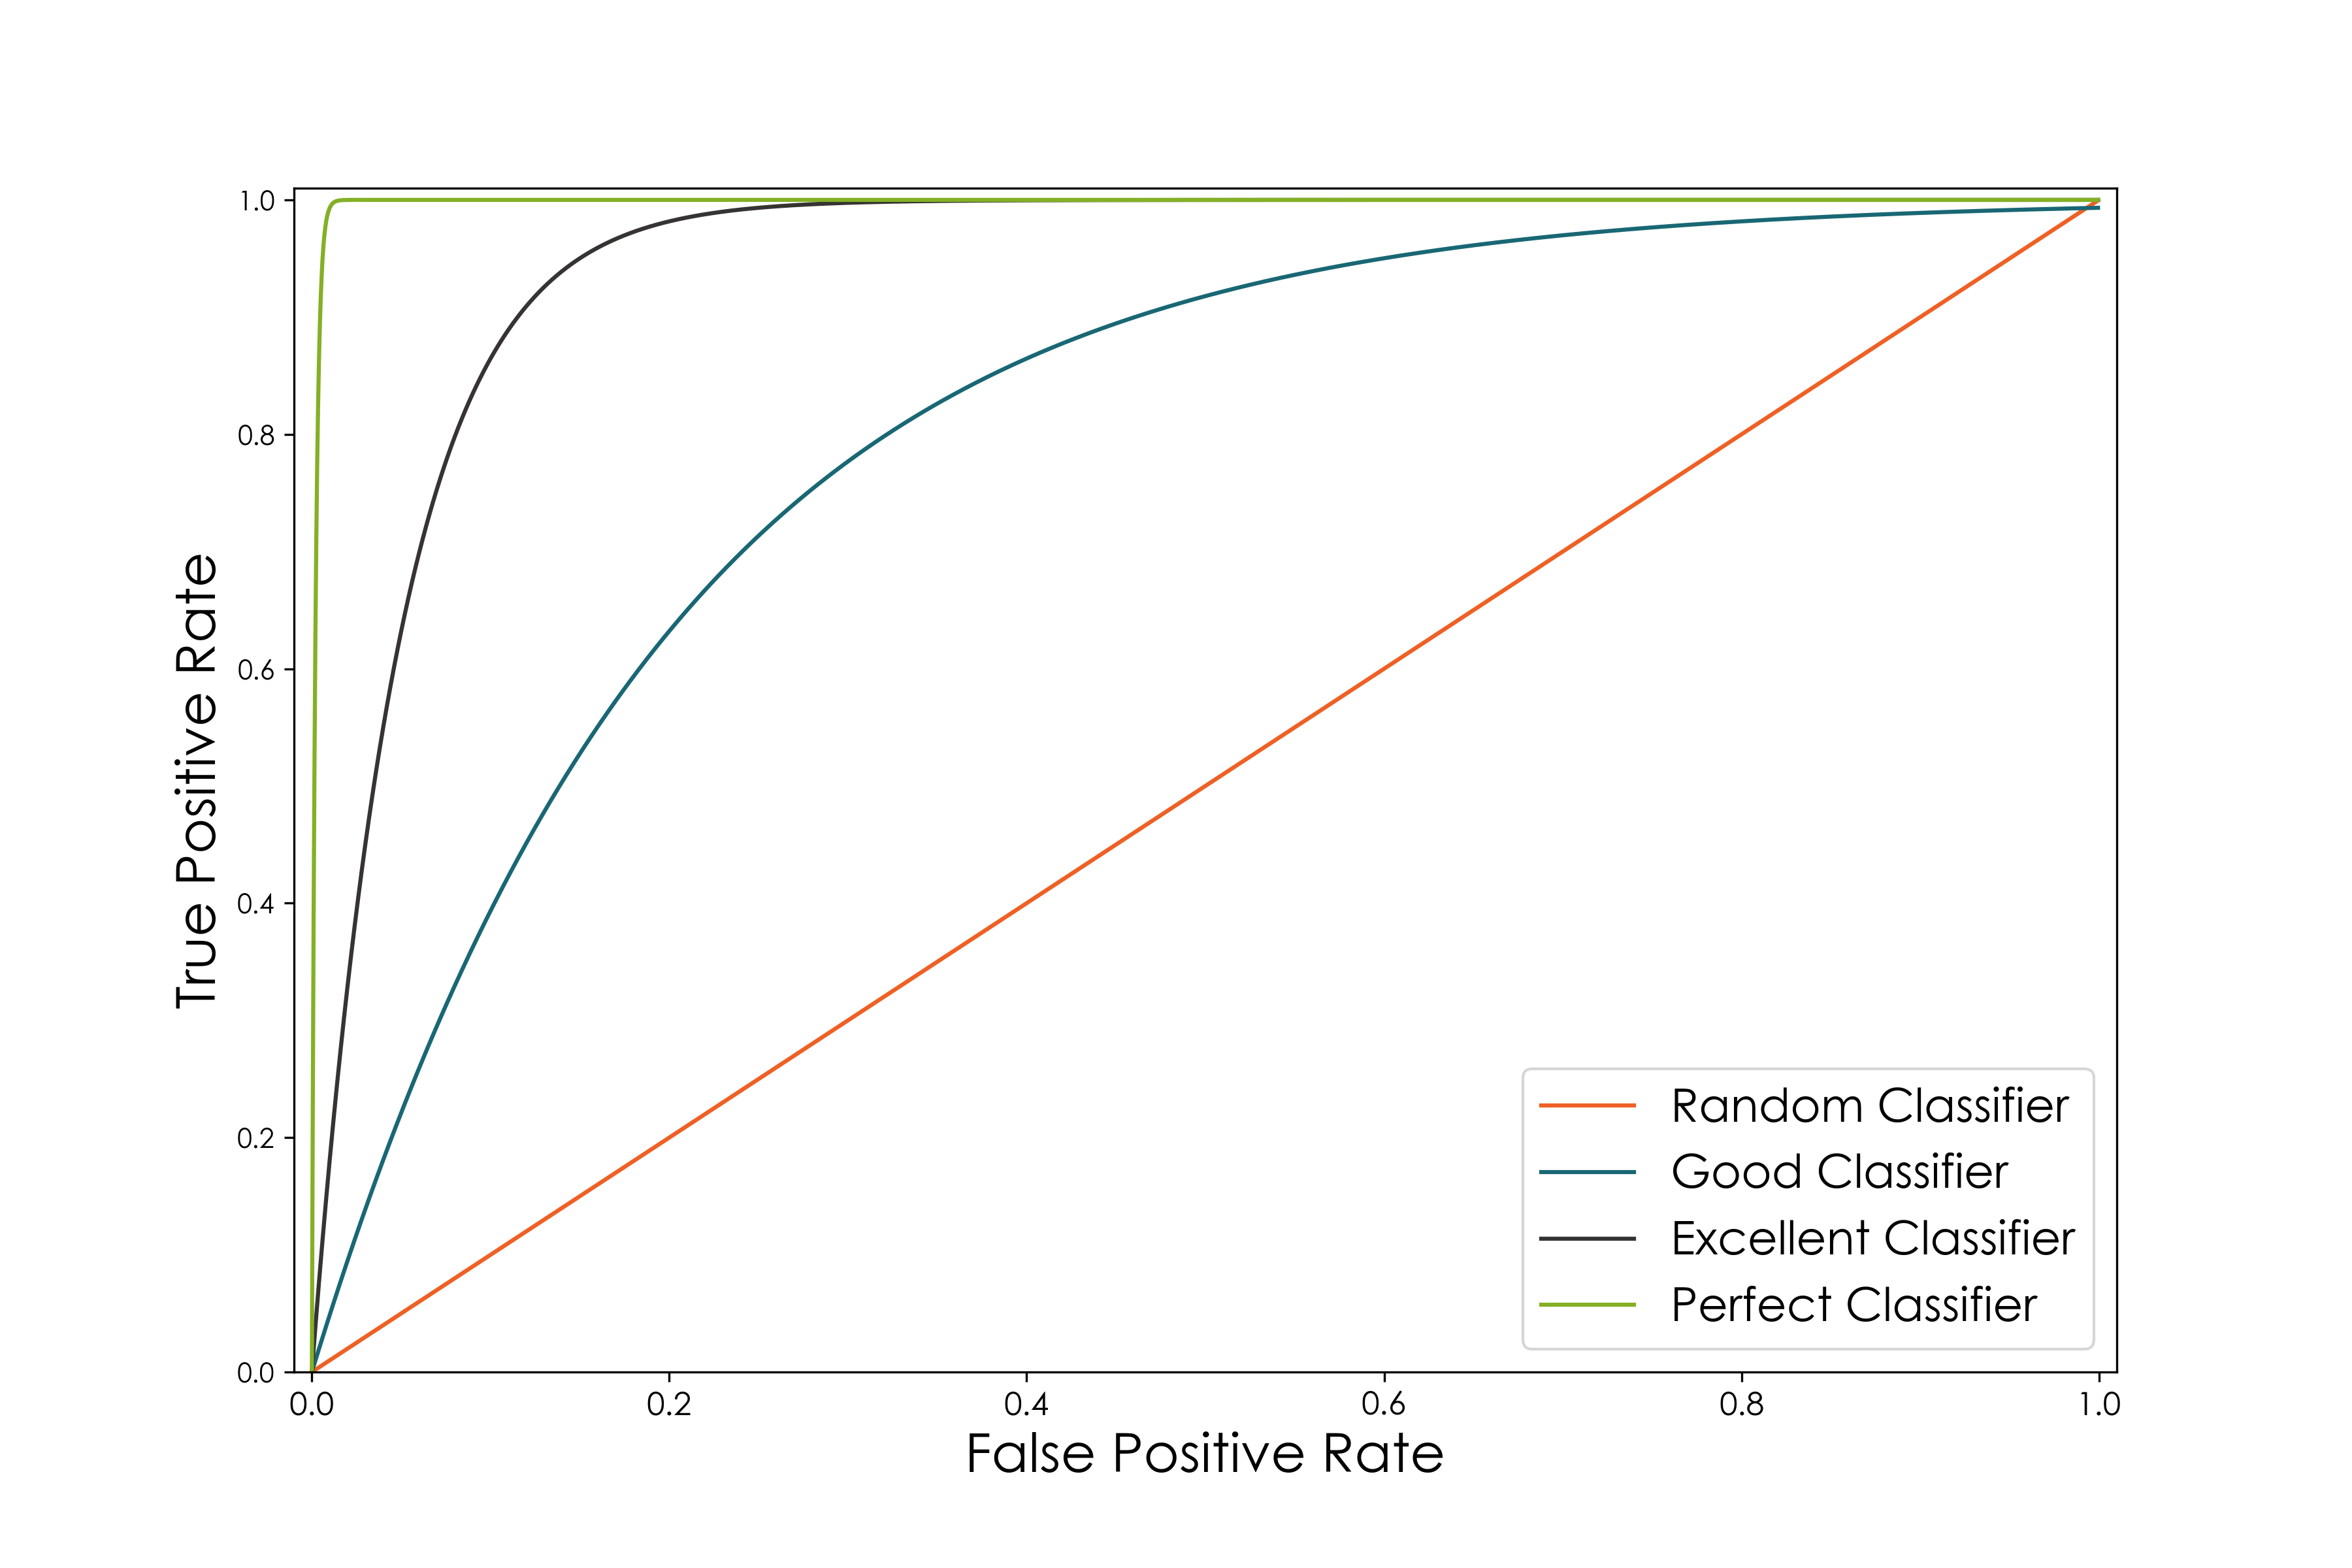
\includegraphics[width=1.0\textwidth]{./figure/chap 5/AUC.png}
\caption{Area Under Curve of Receiver Operating Characteristic (AUC-ROC)}
\label{Fig 5.1}
\end{figure}

\section{Testing Setups}
The prerequisite for building a good machine learning model is to validate its performance of it against unknown data. If not, the model may \emph{overfit} on the given dataset and perform worse in the actual application where we test the model on real-life unknown data. To do so, we generally split the dataset into some sets which are typically known as training set, testing set and so on. The model should not only work well on the training data but also give an accurate prediction on an unknown dataset. To evaluate how well the model is performing on unknown dataset, we employ different splitting techniques for better generalization.

\subsection{Train-test Split}
This is the most common type of the data splitting methods. In this method, we generally divide the dataset into two mutually exclusive sets. One is training set which is used to train the model and includes all the known labels. Another is testing set in which we hide the labels from the model and evaluate how does the model perform on unknown data. The split ratio is a term that defines how much data are in the training set and testing set. A split ratio of 75\% means 75\% of the total data are kept in training set and the rest 25\% data are in testing set. The split ratio is typically chosen between 60\% to 80\%, but a split ratio outside this range may be picked depending on the dataset. Generally, the split ratio keeps increasing with the dataset size.

\begin{figure}[H]
\centering

\includegraphics[width=1.0\textwidth]{./figure/chap 5/Train_test_split.png}
\caption{Train-test split}
\label{Fig 5.2}
\end{figure}

\subsection{Train-validation-test Split}
Sometimes the dataset is divided into three sets instead of two, adding another set known as validation set. This splitting technique is called train-validation-test split. In such a case, the data is first trained on training set and validated on the validation set to evaluate the performance. The model that has the best performance on the validation set is chosen and is tested on the testing set to obtain the actual performance of the model. 

\begin{figure}[H]
\centering

\includegraphics[width=1.0\textwidth]{./figure/chap 5/Train_val_test_split.png}
\caption{Train-validation-test split}
\label{Fig 5.3}
\end{figure}

\subsection{K-fold Cross Validation}
Cross-validation is a statistical splitting method used to estimate the skill of machine learning models. The procedure has a single parameter called $k$ which signifies how many splits will be made. When a particular number for k is selected, it may be substituted for k in the model's reference, such as when k=10 is used to refer to 10-fold cross-validation. 
The general procedure of this method is given below:
\begin{enumerate}
    \item Randomly shuffle the dataset.
    \item Create $k$ groups from the dataset.
    \item For every distinct group:
    \begin{enumerate}
        \item The group should be used as a holdout or test data set.
        \item Use the remaining groupings as the training data set.
        \item Fit the model to the training data, then assess it against the test data.
    \end{enumerate}
    \item Repeat the procedure for $k$ times.
    \item Using a model evaluation metric, summarize the model's skill. 
\end{enumerate}

By following this procedure k-fold cross validation removes the splitting bias which is present in the previous techniques. 

\begin{figure}[H]
\centering
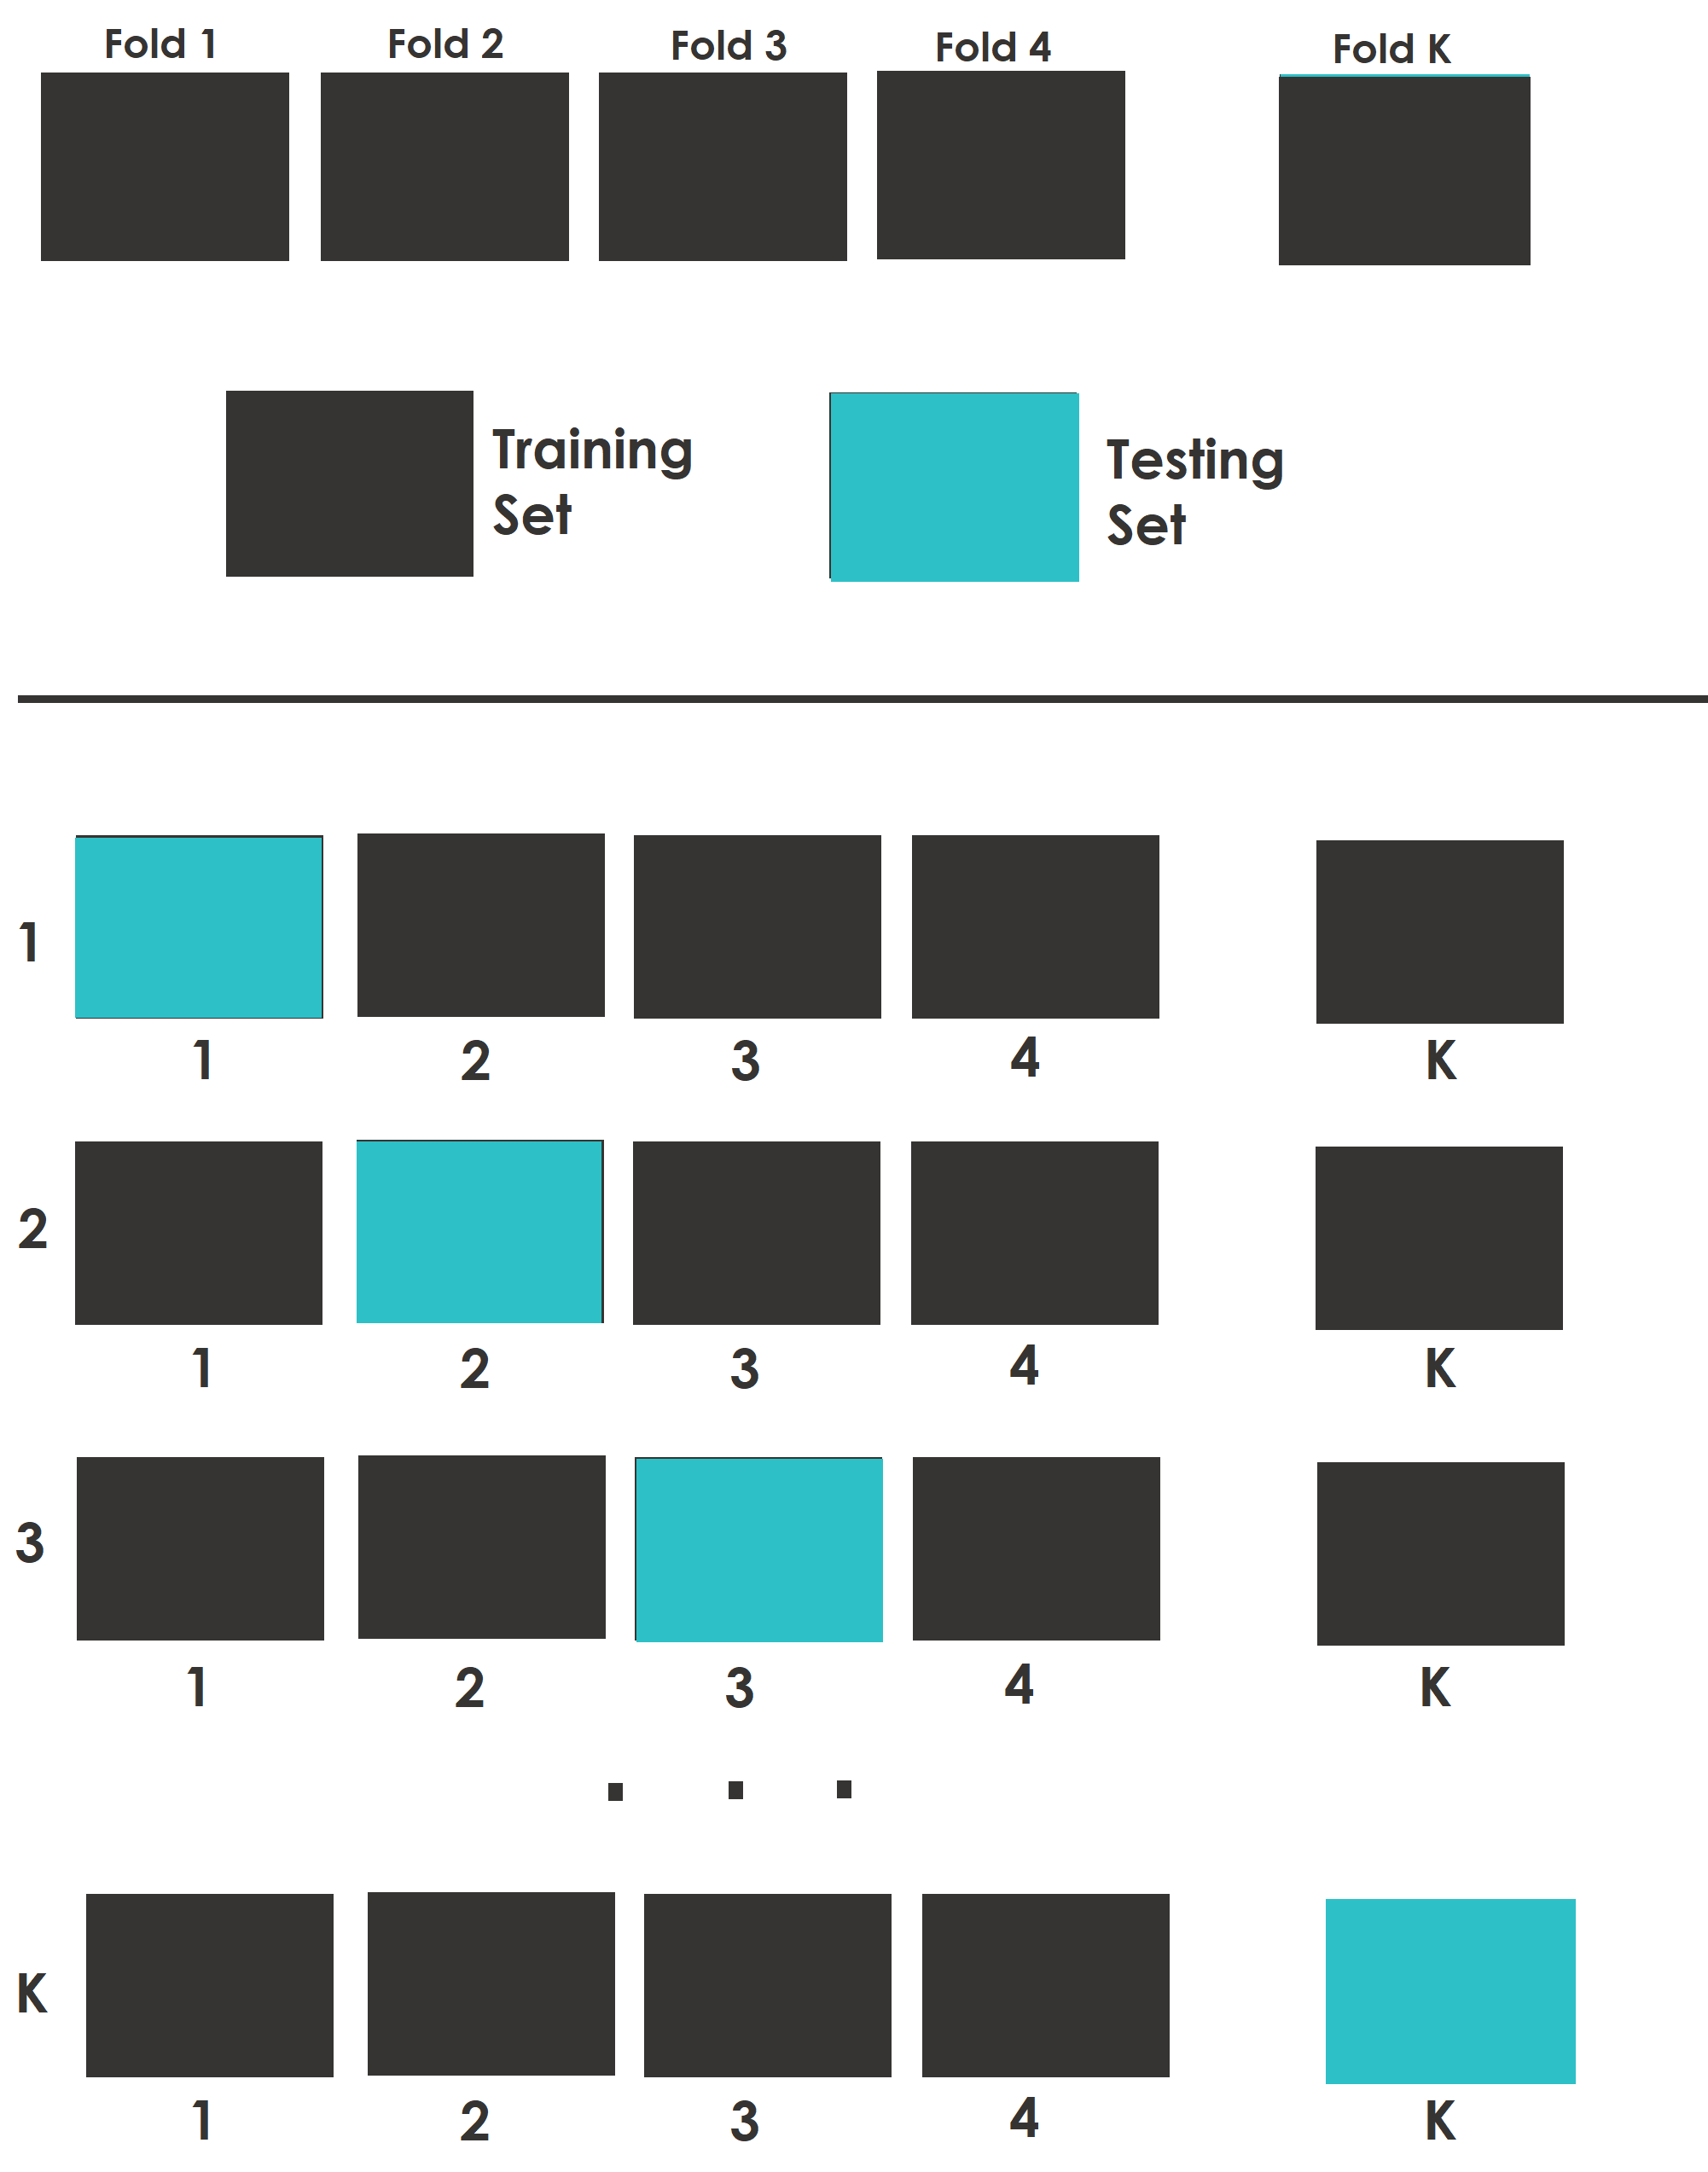
\includegraphics[width=0.8\textwidth]{./figure/chap 5/kfold.png}
\caption{K-fold cross validation}
\label{Fig 5.4}
\end{figure}


\subsection{Leave-One-Out Cross Validation (LOOCV)}
LOOCV is specially used in datasets where data are related to human subjects like in this dataset of human activity recognition. Different subjects carry out different activities in unique ways. Because of this variation, it is harder to predict a new subject's activity. To address this problem, we split the data according to each subject. That means each split contains only one subject's data. Then we perform the cross validation to assess the performance of the model on a new subject.

\section{Results}

\subsection{Fall Detection}
For the fall detection task, we had two classes: fall and non-fall. We experimented with different models and conducted a thorough hyperparameter tuning. Then we evaluated the performance of the models using a 75\% train-test split and a 10-fold cross validation. 
\begin{table}[H]
\caption{Result of fall detection}
\vspace{2mm}
\centering
\begin{tabular}{|c|cc|cc|}
\hline
\multirow{2}{*}{Model}    & \multicolumn{2}{c|}{75\% Train-test split}     & \multicolumn{2}{c|}{10-fold CV}          \\ \cline{2-5} 
                          & \multicolumn{1}{c|}{Accuracy} & F1 score & \multicolumn{1}{c|}{Accuracy} & F1 score \\ \hline
Logistic Regression       & \multicolumn{1}{c|}{0.657}    & 0.632    & \multicolumn{1}{c|}{0.762}    & 0.772    \\
Support Vector Classifier & \multicolumn{1}{c|}{0.938}    & 0.929    & \multicolumn{1}{c|}{0.921}    & 0.922    \\
K Nearest Neighbors       & \multicolumn{1}{c|}{0.923}    & 0.909    & \multicolumn{1}{c|}{0.921}    & 0.924    \\
Random Forest             & \multicolumn{1}{c|}{0.966}    & 0.962    & \multicolumn{1}{c|}{0.967}    & 0.967    \\
Extra Trees               & \multicolumn{1}{c|}{0.980}    & 0.978    & \multicolumn{1}{c|}{0.985}    & 0.985    \\
XGBoost                   & \multicolumn{1}{c|}{0.953}    & 0.947    & \multicolumn{1}{c|}{0.954}    & 0.959    \\ \hline
\end{tabular}
\label{Table 5.1}
\end{table}

Using the \ref{Table 5.1}, we can find the best model is the Extra Trees Classifier which obtained 98.5\% accuracy and F1 score in 10-fold CV and 98\% and 97.8\% accuracy and F1 score in 75\% train-test split. We plotted the confusion matrix of this model for 75\% train-test split.

\begin{figure}[H]
\centering
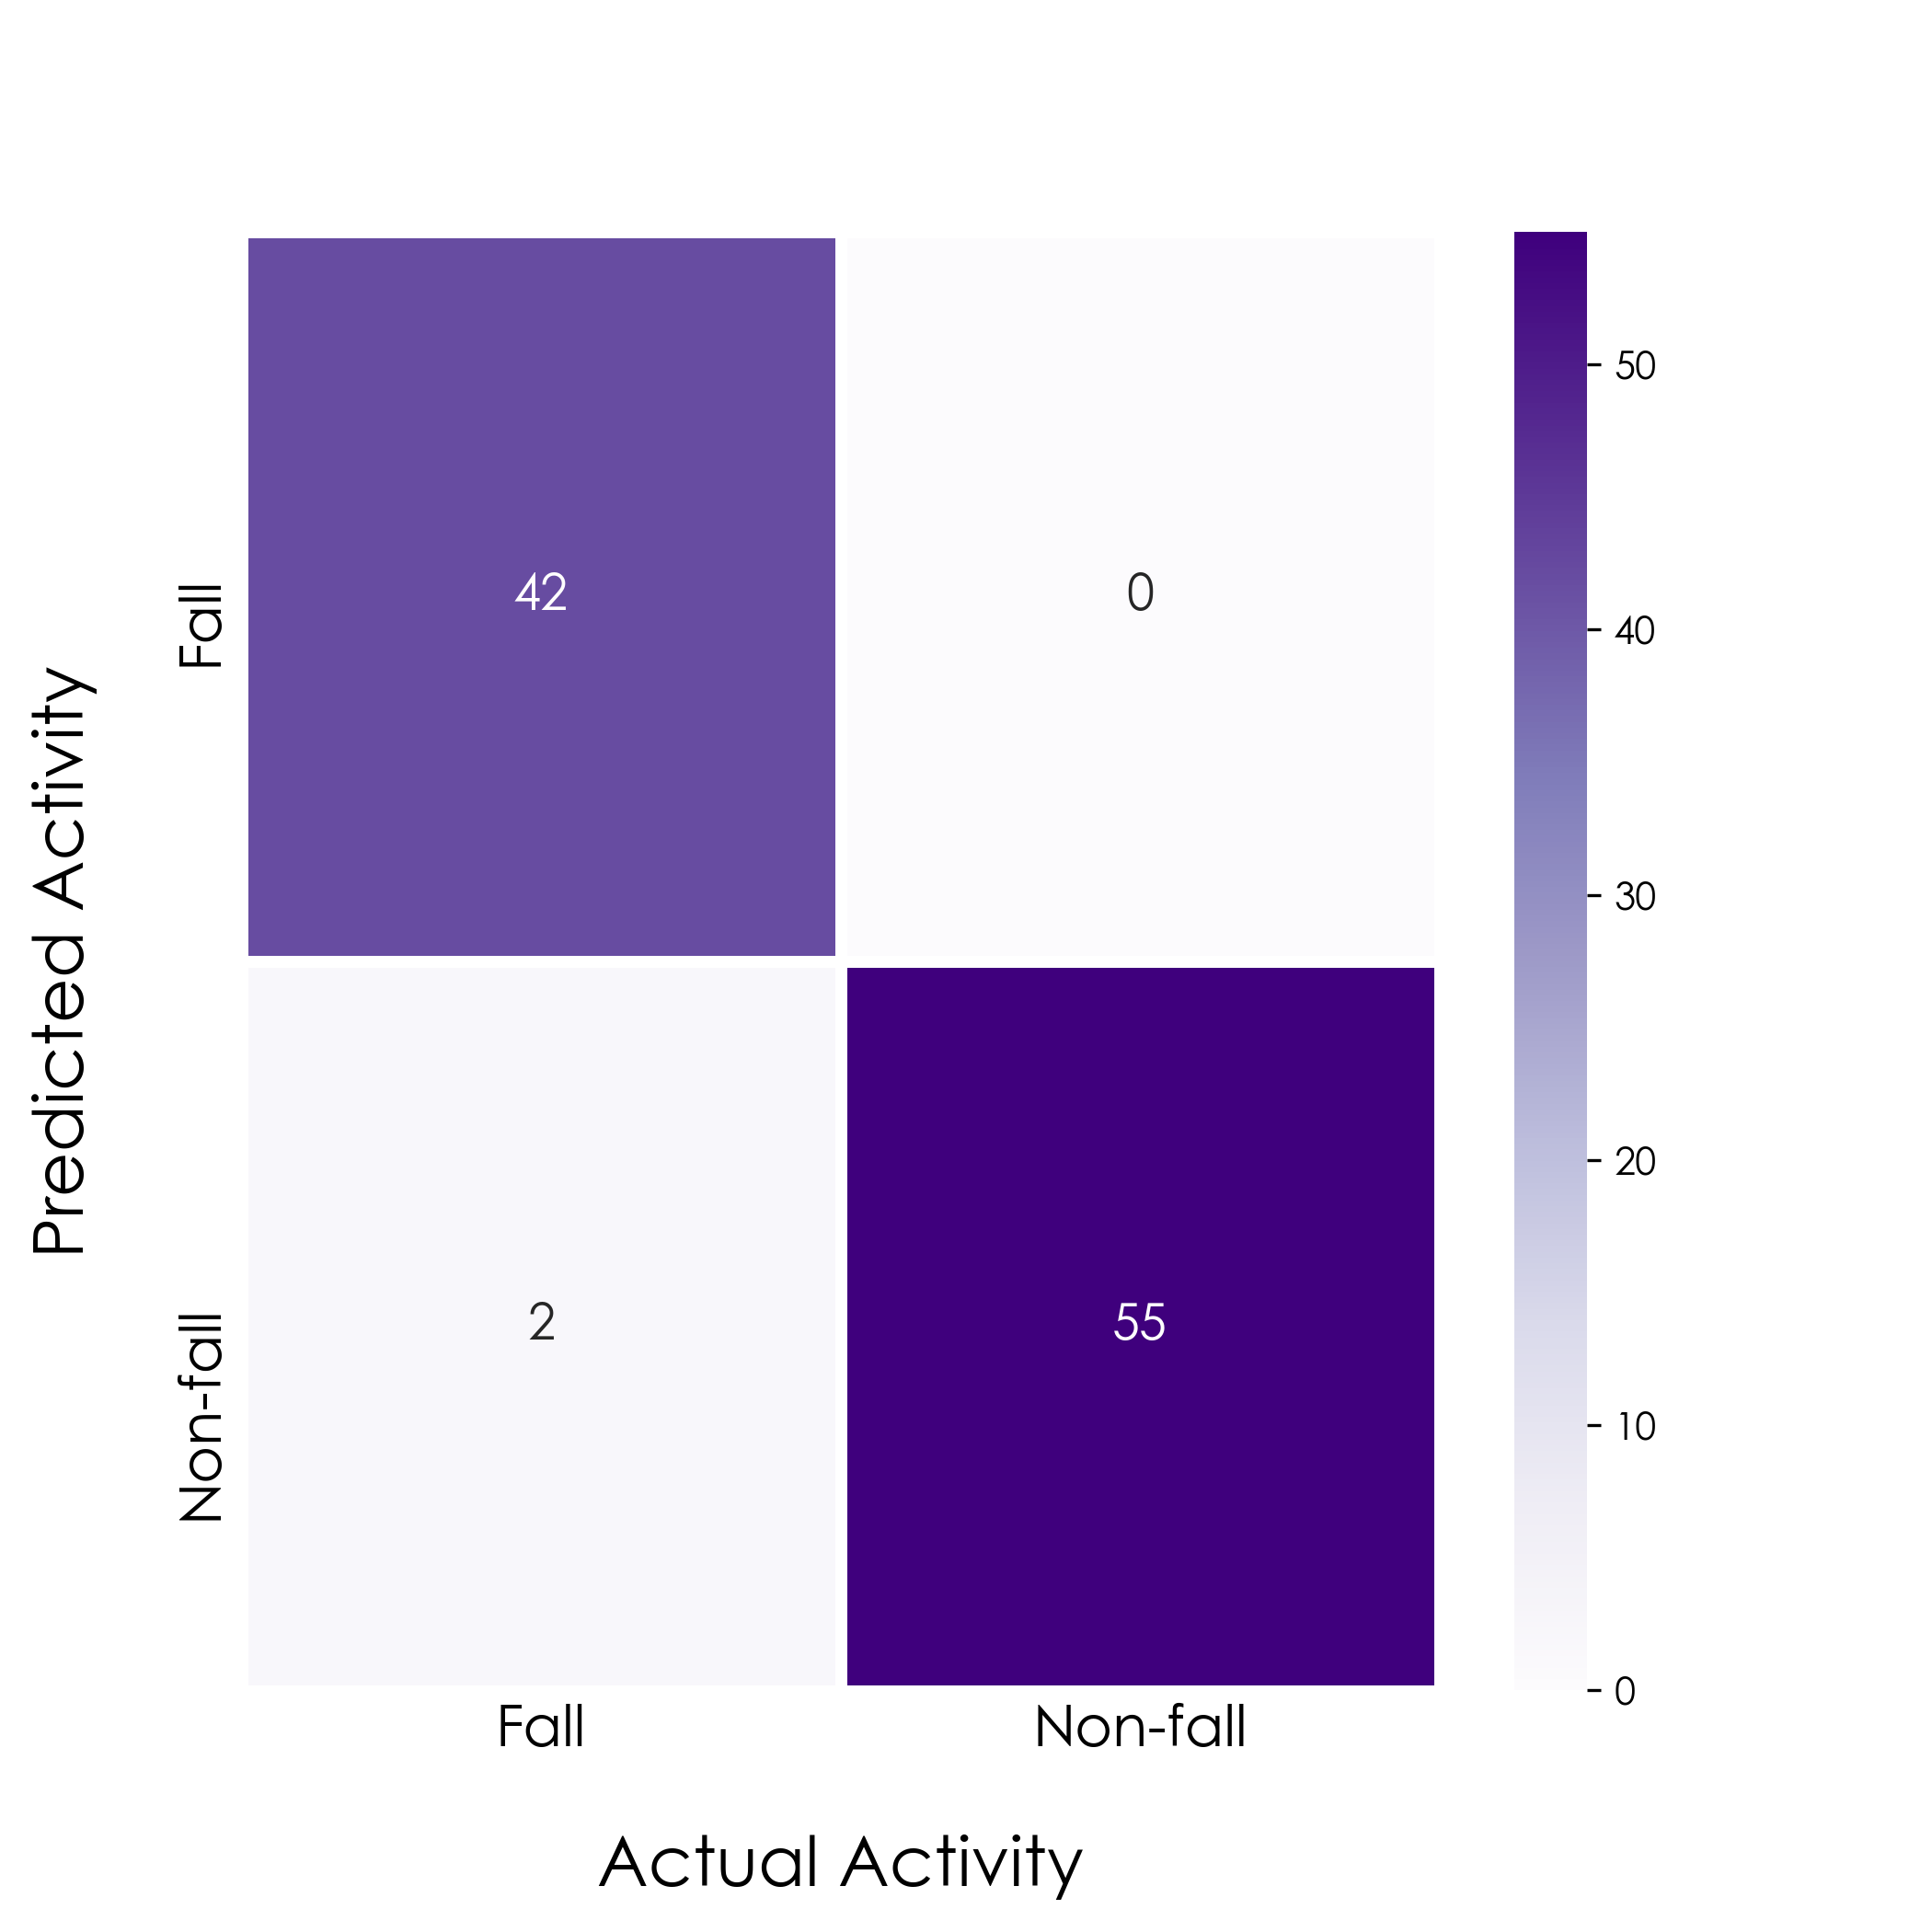
\includegraphics[width=1\textwidth]{./figure/chap 5/conf_binary.png}
\caption{Confusion matrix for fall detection}
\label{Fig 5.5}
\end{figure}

The results of fall detection is summarized in \ref{Fig 5.6}
\begin{figure}[H]
\centering
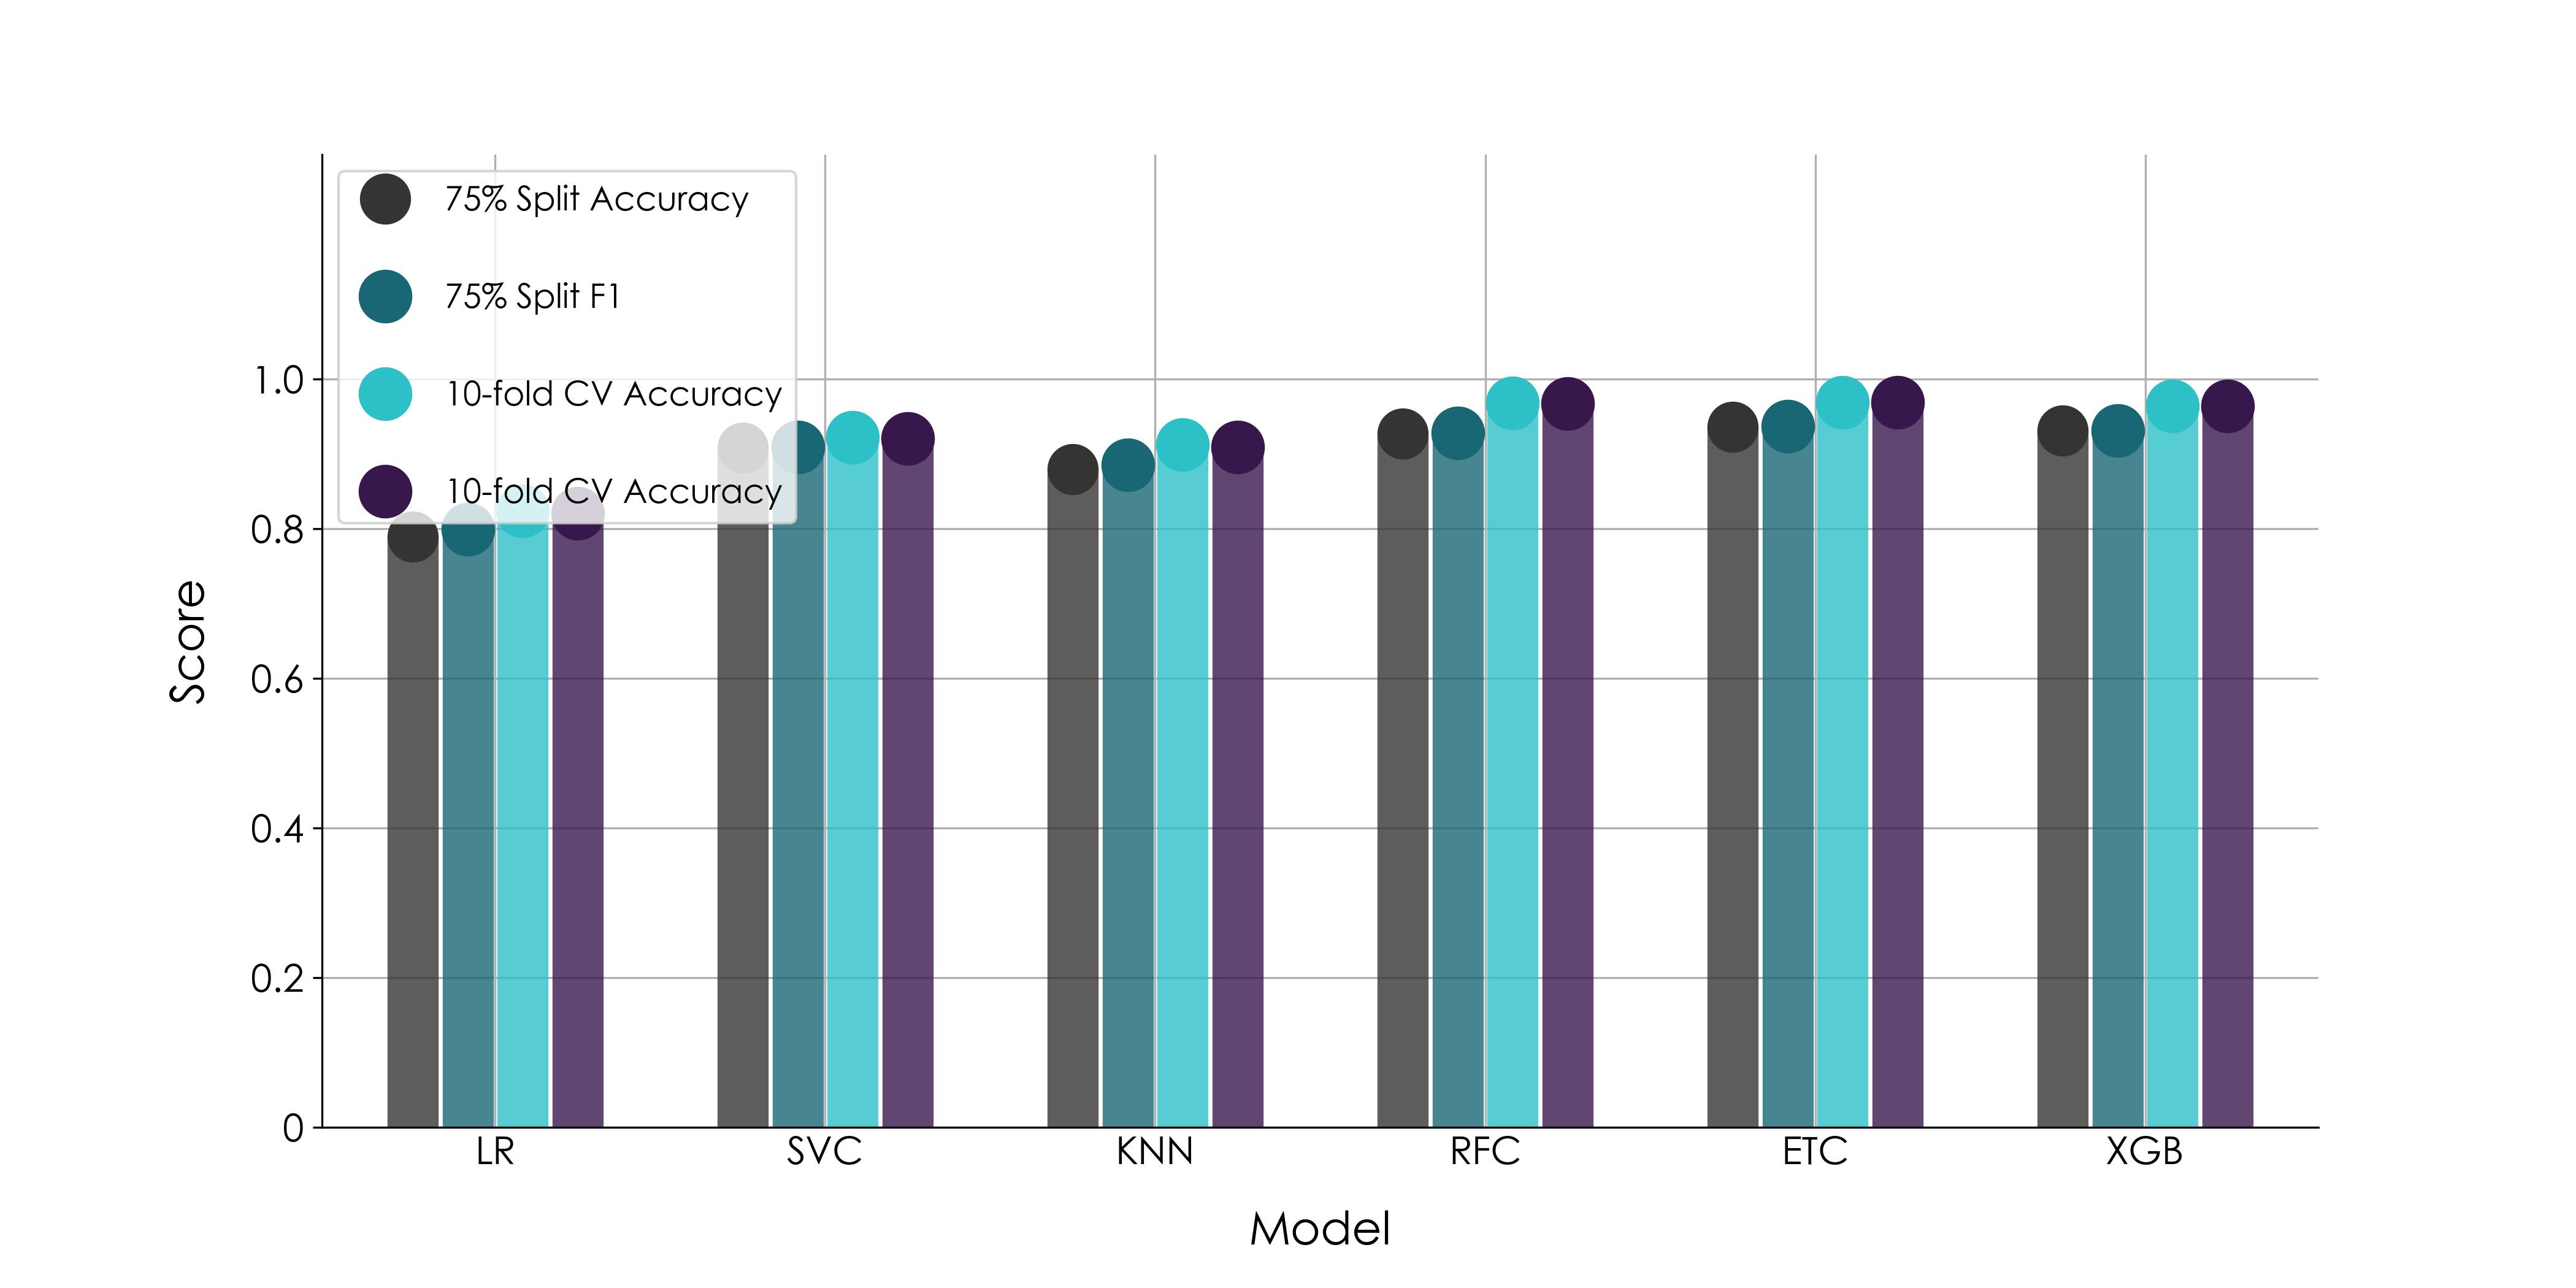
\includegraphics[width=1\textwidth]{./figure/chap 5/binary_model_scores.png}
\caption{Fall detection results}
\label{Fig 5.6}
\end{figure}

\subsection{Human Activity Recognition}
We have five classes of human activity: fall, walk, stand, empty room and presence. We took a similar approach for human activity recognition as fall detection mentioned in the previous sub-section. The results are depicted in table \ref{Table 5.2}.

\begin{table}[H]
\caption{Result of human activity recognition}
\vspace{2mm}
\centering
\begin{tabular}{|c|cc|cc|}
\hline
\multirow{2}{*}{Model}    & \multicolumn{2}{c|}{75\% Train-test split}     & \multicolumn{2}{c|}{10-fold CV}          \\ \cline{2-5} 
                          & \multicolumn{1}{c|}{Accuracy} & F1 score & \multicolumn{1}{c|}{Accuracy} & F1 score \\ \hline
Logistic Regression       & \multicolumn{1}{c|}{0.789}    & 0.799    & \multicolumn{1}{c|}{0.824}    & 0.82     \\
Support Vector Classifier & \multicolumn{1}{c|}{0.908}    & 0.909    & \multicolumn{1}{c|}{0.922}    & 0.92     \\
K Nearest Neighbors       & \multicolumn{1}{c|}{0.879}    & 0.885    & \multicolumn{1}{c|}{0.912}    & 0.909    \\
Random Forest             & \multicolumn{1}{c|}{0.927}    & 0.928    & \multicolumn{1}{c|}{0.968}    & 0.967    \\
Extra Trees               & \multicolumn{1}{c|}{0.936}    & 0.937    & \multicolumn{1}{c|}{0.969}    & 0.969    \\
XGBoost                   & \multicolumn{1}{c|}{0.931}    & 0.931    & \multicolumn{1}{c|}{0.964}    & 0.964    \\ \hline
\end{tabular}
\label{Table 5.2}
\end{table}

Like fall detection, the Extra Trees Classifier gives better results in this task too. The obtained confusion matrix is shown in \ref{Fig 5.7}.

\begin{figure}[H]
\centering
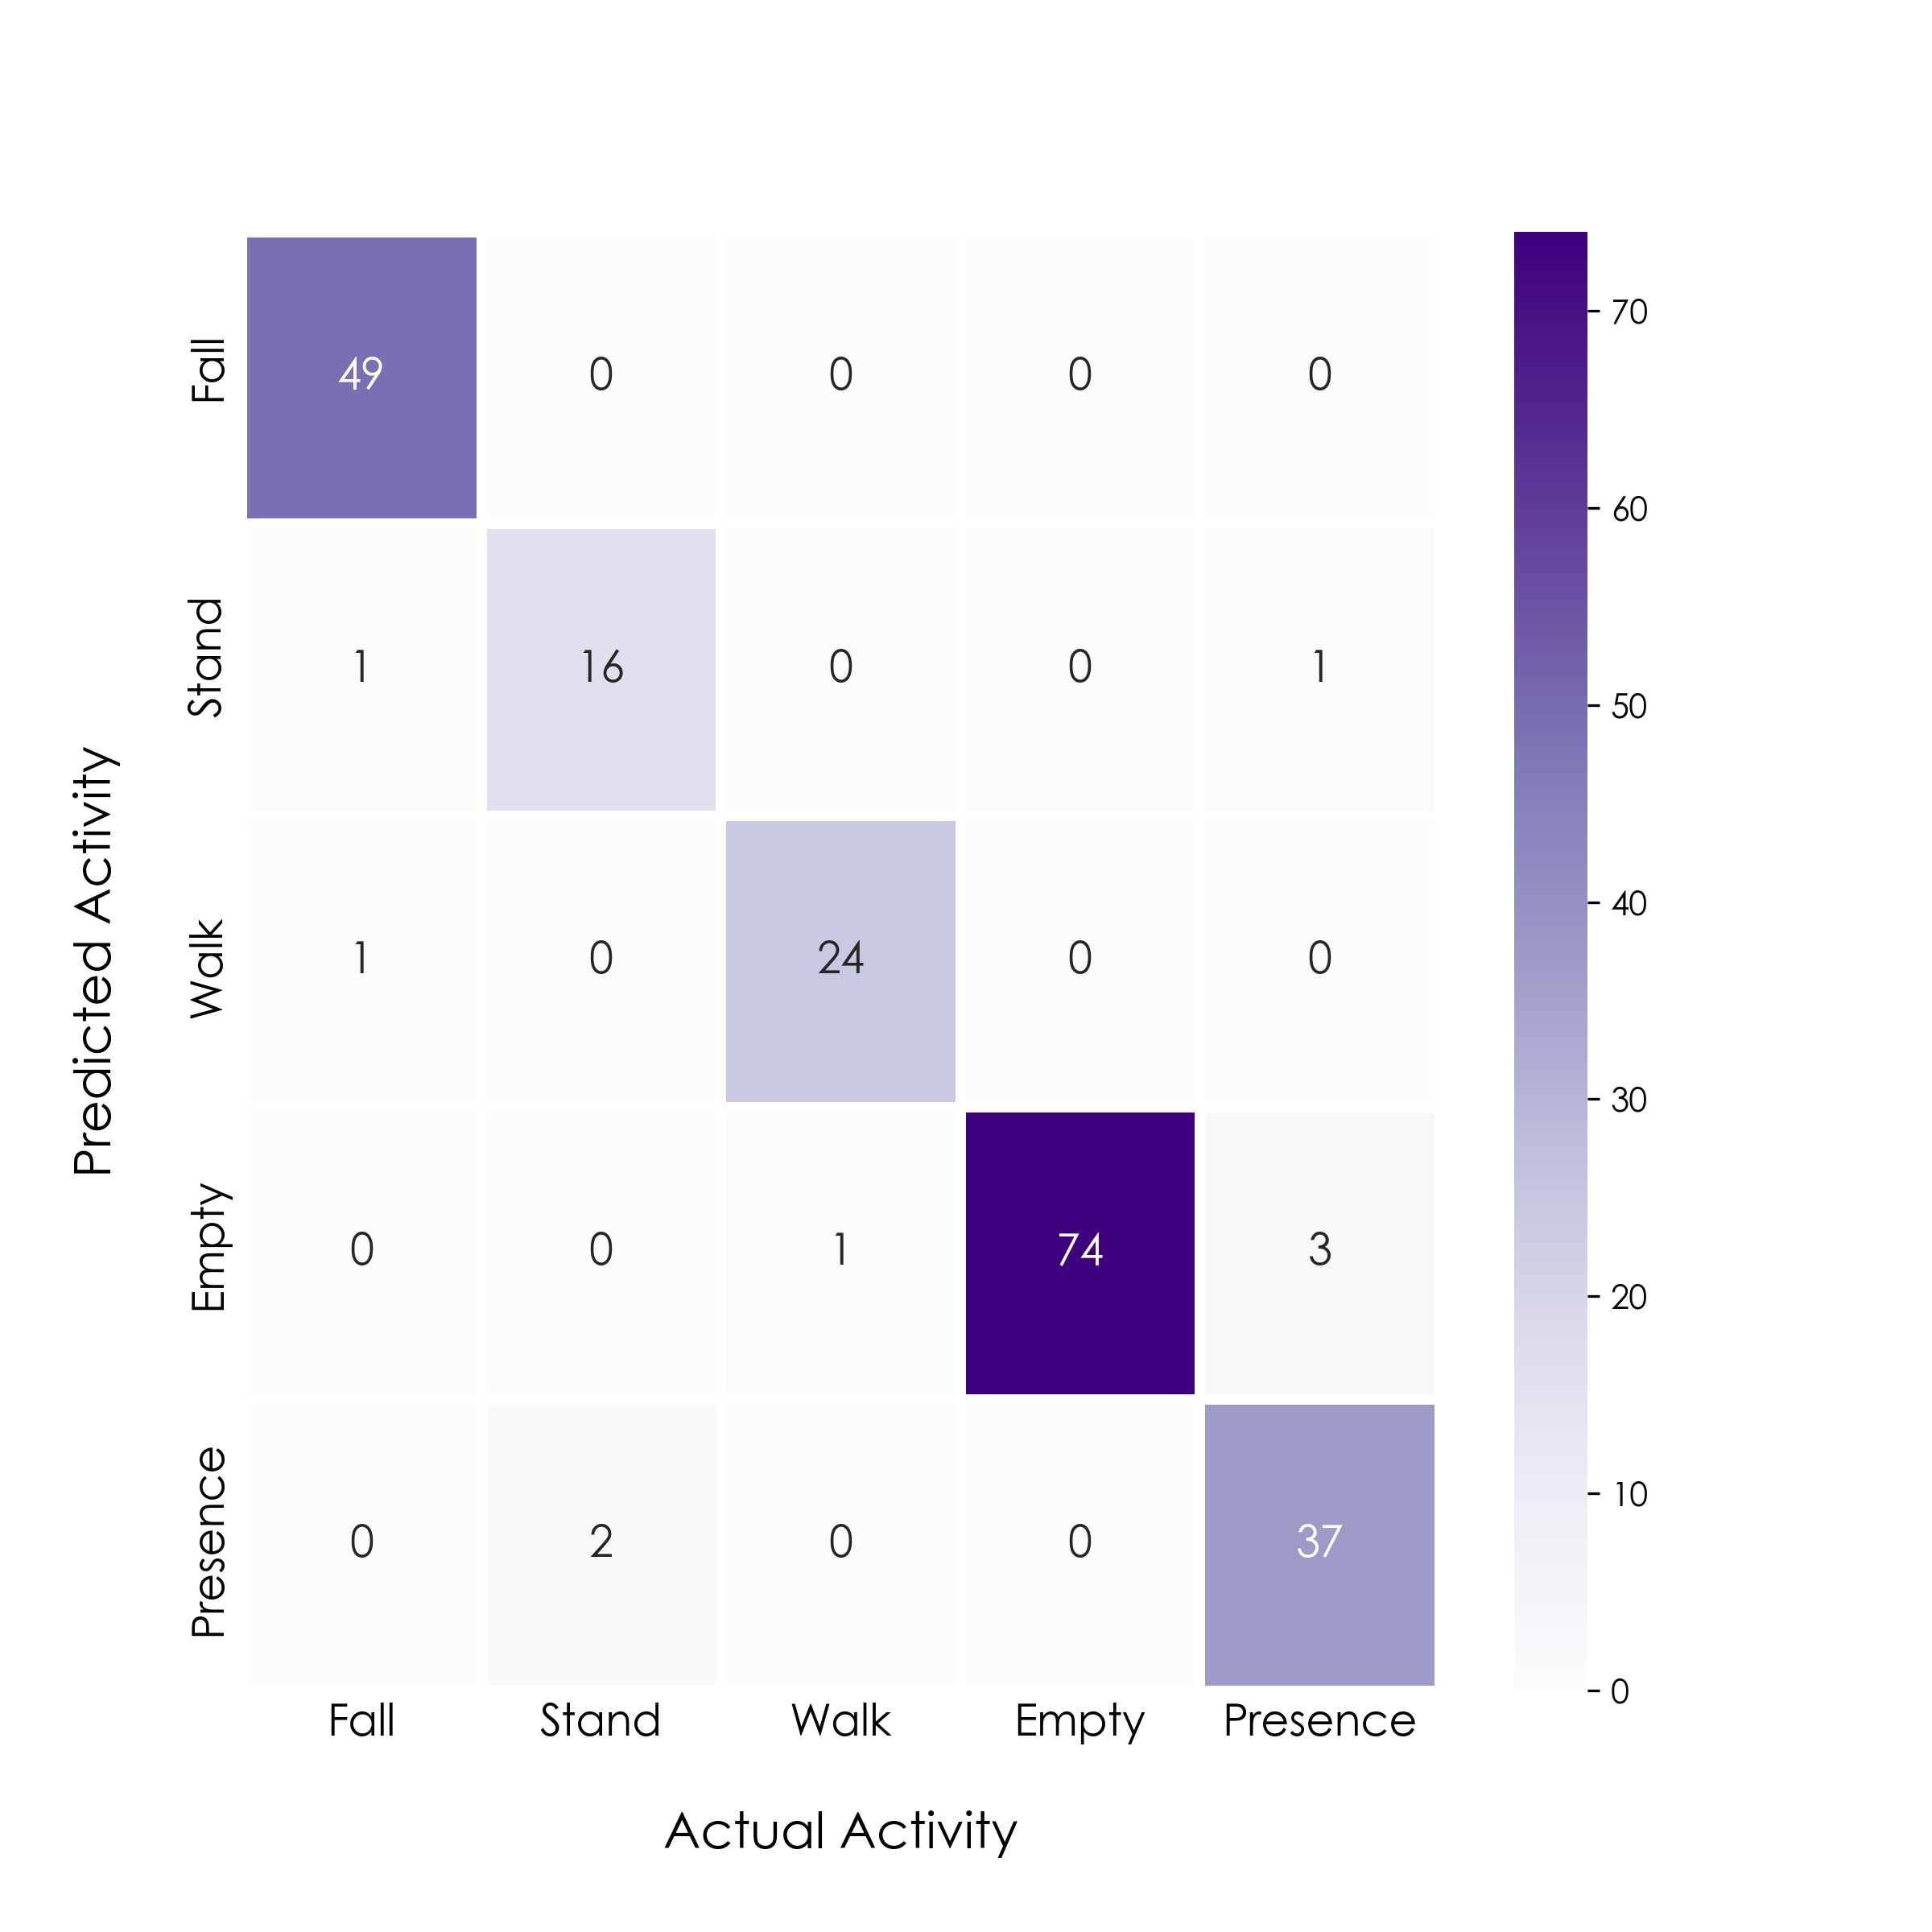
\includegraphics[width=1\textwidth]{./figure/chap 5/conf_multiclass.png}
\caption{Confusion matrix for human activity recognition}
\label{Fig 5.7}
\end{figure}

The results of human activity recognition is summarized in \ref{Fig 5.8}
\begin{figure}[H]
\centering
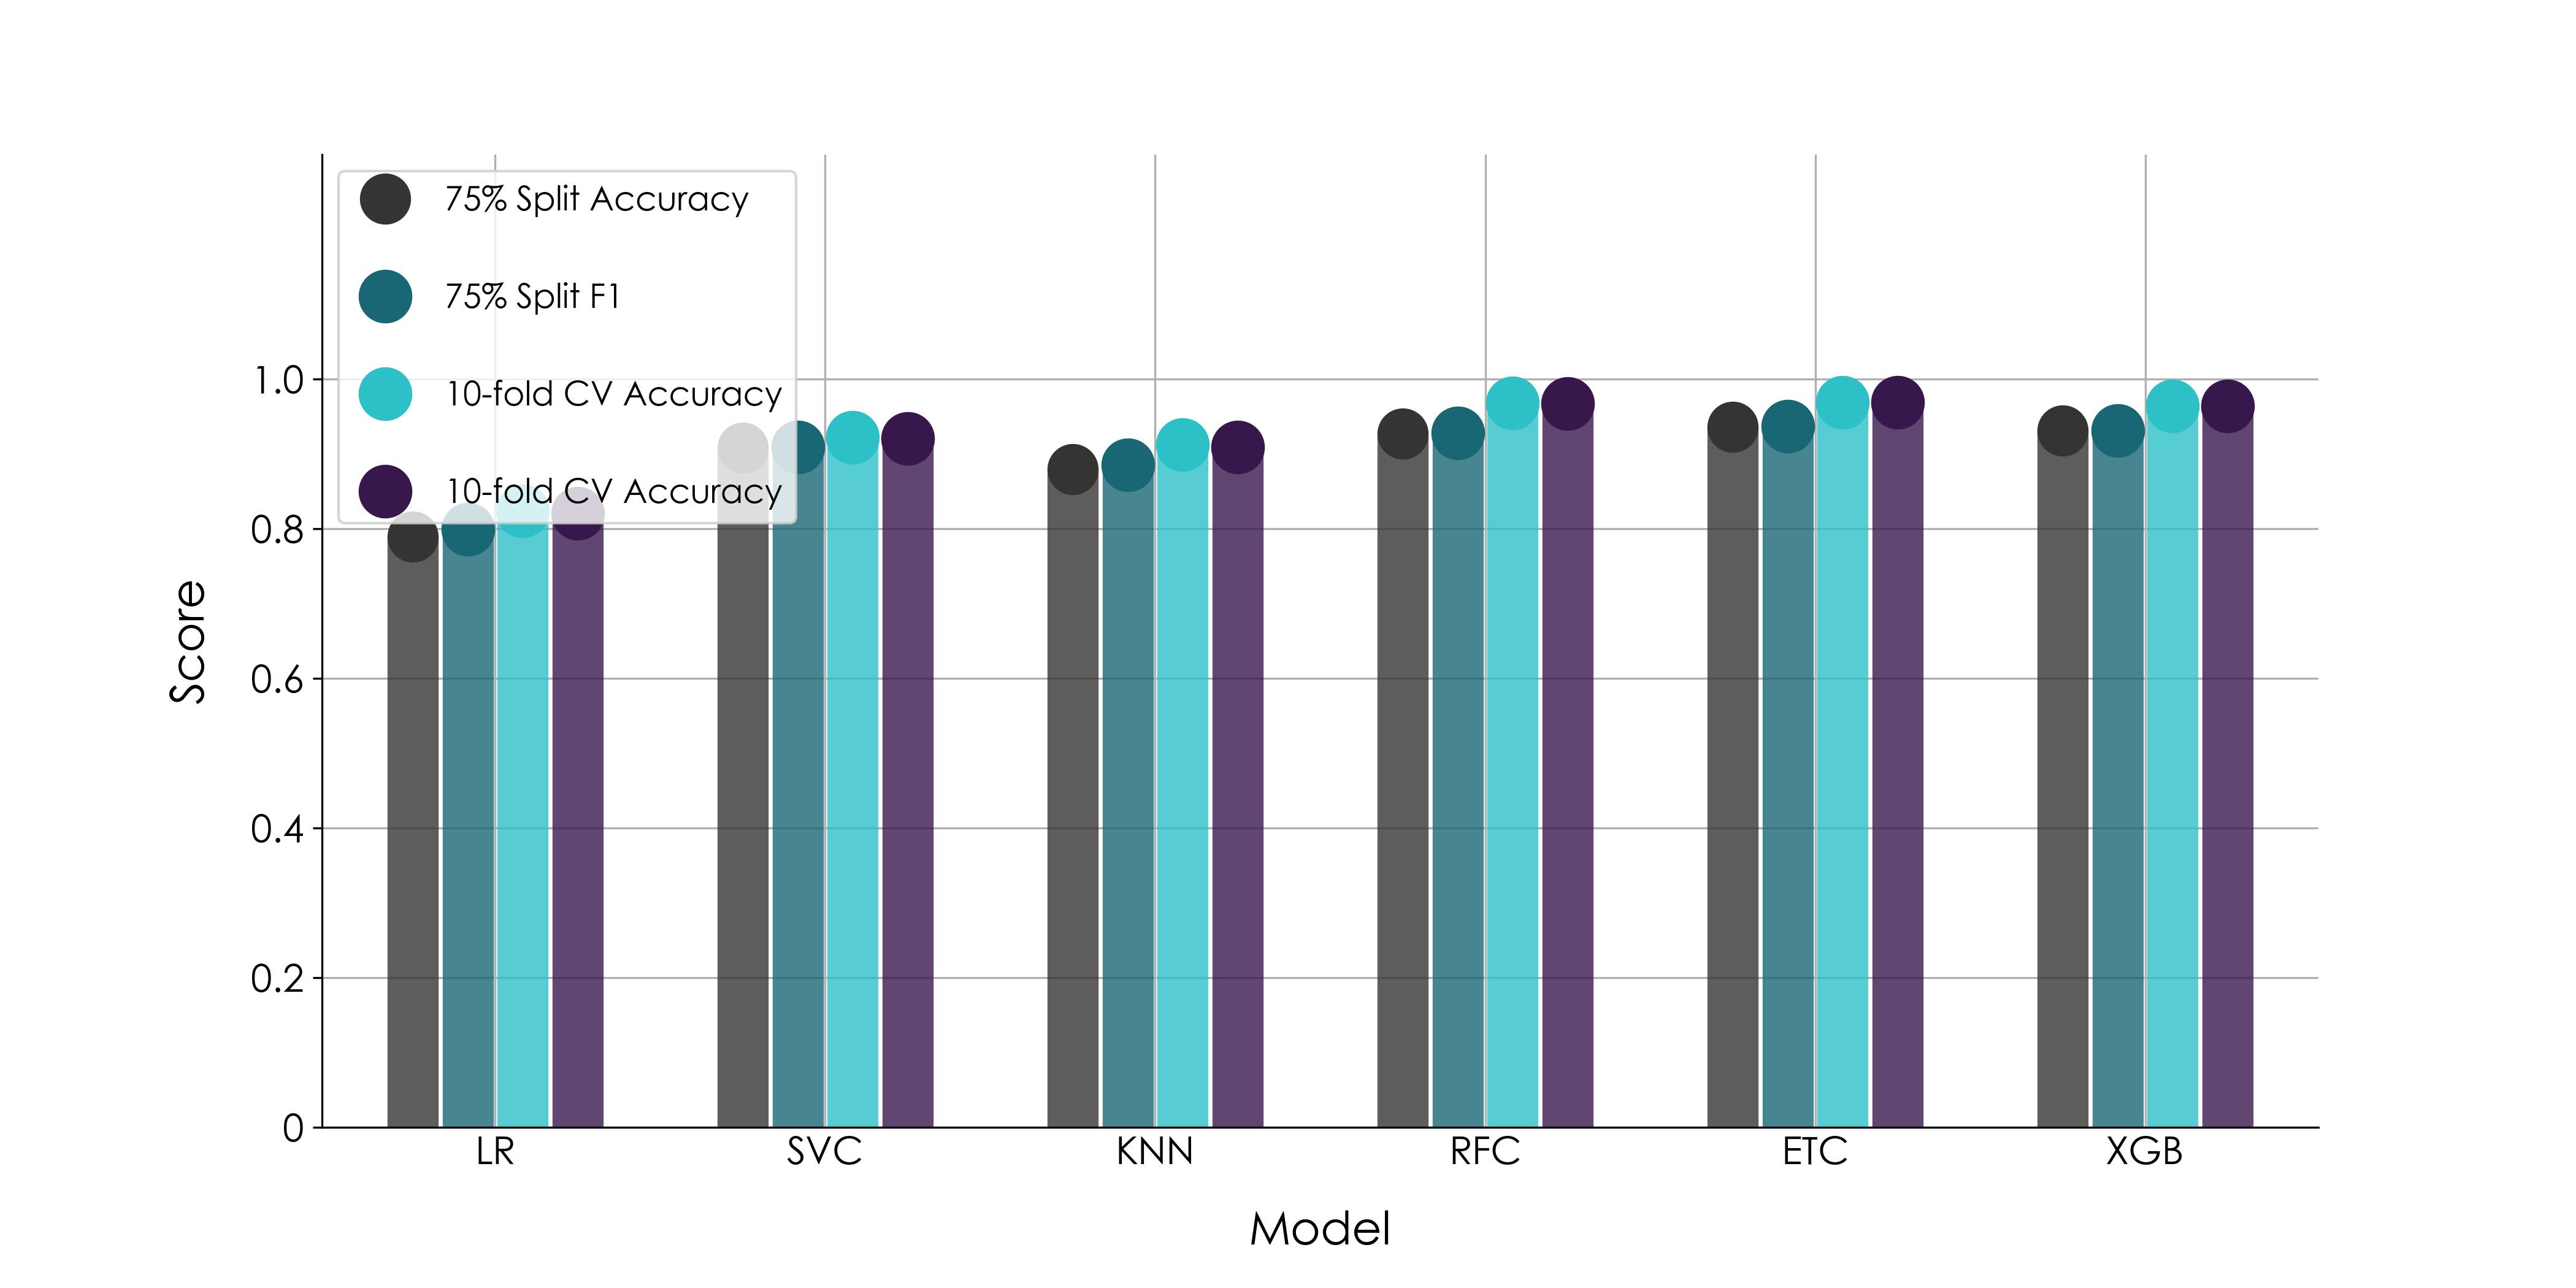
\includegraphics[width=1\textwidth]{./figure/chap 5/multiclass_model_scores.png}
\caption{Human activity recognition results}
\label{Fig 5.8}
\end{figure}

\section{Analysis of in Terms of Speed}
We also conducted an execution time analysis to show that our proposed system is able to run in real-time. The analysis was done on a total of 400 data samples where 300 of them were in the training set and the remaining 100 data samples were in the test set. So, the training data collection time was 1200 seconds and the test data collection time was 400 seconds. We used a lower mid-level laptop with core i5 7200U processor clocked at 2.5 GHz and 8GB RAM to run the time analysis. By looking at \ref{Table 5.3} we can see that, to process the inference data of 400 seconds, the best model Extra trees took only 5 seconds to predict in the multiclass classification problem and 4 seconds to predict in the binary classification problem. So, this system is capable of processing data from up to 80 devices simultaneously  in real-time. Also, the fastest model tested was K Nearest Neighbors which took only 0.1 seconds to predict a data of 400 seconds. So, it can easily be concluded that our proposed system can run and infer in real-time for a number of devices simultaneously.

% Please add the following required packages to your document preamble:
% \usepackage{multirow}
\begin{table}[H]
\caption{Execution time of the models}
\vspace{2mm}
\centering
\begin{tabular}{|c|cc|cc|}
\hline
\multirow{2}{*}{Model}    & \multicolumn{2}{c|}{Binary Classification}                                                                                                        & \multicolumn{2}{c|}{Multi-class Classification}                                                                                                   \\ \cline{2-5} 
                          & \multicolumn{1}{c|}{\begin{tabular}[c]{@{}c@{}}Training \\ time (s)\end{tabular}} & \begin{tabular}[c]{@{}c@{}}Inference \\ time (s)\end{tabular} & \multicolumn{1}{c|}{\begin{tabular}[c]{@{}c@{}}Training \\ time (s)\end{tabular}} & \begin{tabular}[c]{@{}c@{}}Inference \\ time (s)\end{tabular} \\ \hline
Logistic Regression       & \multicolumn{1}{c|}{1.4}                                                          & 0.2                                                           & \multicolumn{1}{c|}{1.6}                                                          & 0.2                                                           \\
Support Vector Classifier & \multicolumn{1}{c|}{2}                                                            & 0.2                                                           & \multicolumn{1}{c|}{2}                                                            & 0.2                                                           \\
K Nearest Neighbors       & \multicolumn{1}{c|}{0.3}                                                          & 0.1                                                           & \multicolumn{1}{c|}{0.4}                                                          & 0.1                                                           \\
Random Forest             & \multicolumn{1}{c|}{15}                                                           & 3                                                             & \multicolumn{1}{c|}{30}                                                           & 6                                                             \\
Extra Trees               & \multicolumn{1}{c|}{15}                                                           & 4                                                             & \multicolumn{1}{c|}{17}                                                           & 5                                                            \\
XGBoost                   & \multicolumn{1}{c|}{18}                                                           & 4                                                             & \multicolumn{1}{c|}{26}                                                           & 6                                                             \\ \hline
\end{tabular}
\label{Table 5.3}
\end{table}

\chapter{CONCLUSION AND FUTURE SCOPE}
 \label{Chapter 6}
 \lhead{ Chapter 6. \emph{Conclusion and Future Scope}}
\label{intro}

In this project, we have proposed a non-contact fall detection and human activity recognition system using embedded devices. The objective of our project was to overcome the drawbacks of the now popular systems that use wearable devices and/or computer vision. Using esp32 and its Wi-Fi capabilities, we have implemented a robust fall detection system that is also able to recognize different activities, and is able to detect if a room is empty. We have analyzed CSI data collected from two esp32 microcontrollers and gone through an elaborate process of cleaning, preprocessing, feature extraction, feature selection and classification using various machine learning models. Through this process, we were able to perform accurate human activity recognition and fall detection. The use of embedded devices made the system open to heavy modifications and lowered its deployment cost, making it highly flexible and affordable.

\section{Discussion}
In this project, we conducted two different tasks and achieved great accuracy. For the first task, fall detection, the dataset is quite balanced. But for the human activity recognition task, the dataset was moderately unbalanced which led to lower accuracy. The confusion matrices in \ref{Fig 5.5} and \ref{Fig 5.7} also depict the same fact.

Although our system is able to recognize different human activities including falls as shown in Chapter 5, our primary goal for this project is fall detection. The reason behind this is that no CSI-based system is able to localize the activities, so the opportunity for real world application is limited for most activities. We can also see from the works of Li et el.\cite{8873550} that accuracy of Wi-Fi CSI-based activity detection systems drops considerably when multiple users perform different activities at the same time. But in case of fall activity, these limitations are irrelevant as in an event of a fall, immediate attention is required regardless.


\section{Future Scopes}
Our proposed system is effective, yet has much room for improvement. The limitations we aim to overcome and the improvements we want to implement in the future are as follows:

\begin{enumerate}
  \item The devices we have used to implement the system use PCB antennas which are not very effective. Using external omnidirectional antennas would increase the effectiveness of the antenna even more.
  
  \item We were able to send and receive packets from one device to another only at relatively small distances and in LoS condition. The reason behind this is that the devices are low power consuming devices. Designing a device that is able to send more powerful signals will solve these problems. 

  \item Designing an enclosure that houses a power system would allow deploying the system easily in various locations.
  
  \item We have only collected data in a controlled environment. Collecting and analyzing data from uncontrolled environments where a lot more moving objects are present would make the system more robust.

  \item Implementing some sort of GUI or interfacing the system with other devices such as smart phones would make this system more user friendly.
  
  \item Although we have been able to successfully recognize different activities, we are unable to localize the activity. This can be done by using multi-dimensional information such as ToF(Time of Flight), AoA(Angle of arrival) and Doppler shift\cite{mDTrack}.
  
\end{enumerate}


 

%\input{./Chapters/Chapter7} 



\addtocontents{toc}{\vspace{1em}}  % Add a gap in the Contents, for aesthetics
\backmatter

%% ----------------------------------------------------------------
\label{Bibliography}
\lhead{\emph{Bibliography}}  % Change the left side page header to "Bibliography"
\bibliographystyle{IEEEtran}
\bibliography{IEEEabrv,mybib}
\clearpage
\begin{appendix}
\addtocontents{toc}{\protect\setcounter{tocdepth}{1}}
\makeatletter
\addtocontents{toc}{%
  \begingroup
  \let\protect\l@chapter\protect\l@section
  \let\protect\l@section\protect\l@subsection
}
\makeatother

\chapter{Appendix A: List of Acronyms}

\lhead{Appendix A. \emph{List of Acronyms}}


\begin{table}[H]
\label{tab:appendix}
\centering
\begin{tabular}{ll}


\textbf{CSI}    & Channel State Information             \\
\textbf{LOS}    & Line of Sight scenario                \\
\textbf{SVM}    & Support Vector Machine          \\
\textbf{LSTM}   & Long Short-Term Memory                      \\
\textbf{NIC}    & Network Interface Card                  \\
\textbf{DWT}    & Discrete Wavelet Transform              \\
\textbf{PCA}    & Principal Component Analysis                  \\
\textbf{IEEE}   & Institute of Electrical and Electronics Engineers      \\
\textbf{AP}     & Access Point             \\
\textbf{WMA}    & Weighted Moving Average                       \\
\textbf{ICA}    & Independent Component Analysis  \\
\textbf{CNN}    & Convolutional Neural Networks             \\
\textbf{ULP}    & Ultra-Low Power              \\
\textbf{RAM}   & Random Access Memory                \\
\textbf{ROM}    & Read Only Memory                  \\
\textbf{EDR}   & Enhanced Data Rate   \\
\textbf{BLE}  & Bluetooth Low Energy  \\
\textbf{SPI}  & Serial Peripheral Interface      \\
\textbf{MAC} & Media Access Control           \\
\textbf{DMA}  & Direct Memory Access      \\
\textbf{PWM}  &  Pulse Width Modulation      \\
\textbf{WPA}  &     Wi-Fi Protected Access  \\

\end{tabular}
\end{table}

\begin{table}[H]
\centering
\begin{tabular}{ll}
\textbf{WLAN}  &    Wireless Local Area Network   \\
\textbf{WAPI}  &    WLAN Authentication and Privacy Infrastructure   \\
\textbf{ECC}  &    Elliptic Curve Cryptography   \\
\textbf{RNG}  &     Random Number Generator   \\
\textbf{GPIO}  &    General-Purpose Input/Output   \\
\textbf{RTC}  &     Real Time Clock  \\
\textbf{OFDM}  &    Orthogonal Frequency Division Multiplexing   \\
\textbf{QAM}  &    Quadrature Amplitude Modulation   \\
\textbf{RSSI}  &     Received Signal Strength Indication  \\
\textbf{MCS}  &      Modulation Coding Scheme  \\
\textbf{MIMO}  &    Multiple-Input Multiple-Output   \\
\textbf{UART}  &    Universal Asynchronous Receiver Transmitter   \\
\textbf{MCU}  &     Micro Controller Unit  \\
\textbf{CPU}  &     Central Processing Unit  \\
\textbf{RF}  &      Radio Frequency \\
\textbf{LAN}  &    Local Area Network   \\
\textbf{MU-MIMO}  &     Multi-User MIMO  \\
\textbf{DSL}  &    Digital Subscriber Line   \\
\textbf{RL}  &      Reinforcement Learning \\
\textbf{ICMP}  &   Internet Control Message Protocol    \\
\textbf{PCB}  &     Printed Circuit Board  \\
\textbf{BPSK}  &     Binary Phase-Shift keying  \\
\textbf{FFT}  &      Fast Fourier Transform \\
\textbf{DFT}  &      Discrete Fourier Transform \\
\textbf{IDFT}  &     Inverse Discrete Fourier Transform \\
\textbf{STFP}  &     Short-Time Fourier Transform  \\
\textbf{SDR}  &      Software Defined Radio \\
\textbf{CWT}  &      Continuous Wavelet Transform \\
\textbf{IDWT}  &       Inverse Discrete Wavelet Transform\\
\end{tabular}
\end{table}


\begin{table}[H]
\centering
\begin{tabular}{ll}
\textbf{PCC}  &      Pearson's Correlation Coefficient \\
\textbf{DT}  &      Decision Tree \\
\textbf{TP}  &       True Positive\\
\textbf{FP}  &      False Positive \\
\textbf{TN}  &      True Negative \\
\textbf{FN}  &      False Negative \\
\textbf{TPR}  &     True Positive Rate  \\
\textbf{FPR}  &     False Positive Rate  \\
\textbf{FNR}  &     False Negative Rate  \\
\textbf{AUC}  &     Area Under Curve  \\
\textbf{ROC}  &     Receiver Operating Characteristic  \\
\textbf{CV}  &      Cross Validation \\
\textbf{LOOCV}  &      Leave-One-Out Cross Validation \\
\textbf{LR}  &      Logistic Regression \\
\textbf{SVC}  &      Support Vector Classifier \\
\textbf{KNN}  &      K Nearest Neighbors \\
\textbf{RFC}  &      Randon Forest Classifier \\
\textbf{ETC}  &     Extra Trees Classifier  \\
\textbf{XGB}  &     XGBoost  \\
\textbf{GUI}  &     Graphical User Interface  \\
\end{tabular}
\end{table}

\end{appendix}



\end{document}  % The End
%% ----------------------------------------------------------------

